\documentclass[a4paper,11pt]{article}

\usepackage[margin=2.4cm]{geometry}
\usepackage{ctex}
\usepackage{amsmath,amssymb}
\usepackage{booktabs}
\usepackage{array}
\usepackage{enumitem}
\usepackage{float}
\usepackage{graphicx}
\usepackage{xcolor}
\usepackage{xurl}
\usepackage{hyperref}
\usepackage{caption}

\graphicspath{{figures/}}
\hypersetup{
  colorlinks=true,
  linkcolor=blue!60!black,
  citecolor=blue!60!black,
  urlcolor=blue!60!black
}
\setlist[itemize]{nosep,leftmargin=1.8em}
\setlist[enumerate]{nosep,leftmargin=1.8em}

\title{\textbf{190 MeV/u 极化氘核破裂实验对 $\gamma$ 约束的技术报告}}
\author{Baiting Tian}
\date{2026 年 6 月 11 日}

\begin{document}
\maketitle

\section*{数据口径}

\begin{itemize}
  \item 本地代码仓库: \texttt{/home/tian/workspace/dpol/smsimulator5.5}
  \item NEBULA-Plus 重建样本: {\footnotesize\path{/home/tian/workspace/sshDir/spana03/Dpol_smsimulator/data/reconstruction/nebulaplus_nn_joint_20260609_012854}}
  \item folding 诊断表: \texttt{checks/observables/folding\_diagnostics/}
  \item 本报告图表: \texttt{docs/reports/gamma\_constraint\_20260611/figures/}
\end{itemize}

\paragraph{数据溯源}
三级流水线 (本报告所有图表基于同一套样本): \\
1. QMD 模拟: d+Sn 190 MeV/u, $\gamma=\{0.5,0.6,0.7,0.8\}$, 靶 Sn112+Sn124, ypol (phi\_random) + zpol (b\_discrete)。 \\
2. breakup 提取: \texttt{breakup\_nn\_targetframe\_20260607\_180428} (2026-06-07 18:04)。 \\
3. NEBULA-Plus + PDC NN joint 重建: \texttt{nebulaplus\_nn\_joint\_20260609\_012854} (2026-06-09 01:28)。 \\
所有图表脚本 (\texttt{make\_cut\_diagnostics\_figures.py}, \texttt{plot\_nebulaplus\_reco.py}) 用 uproot 直接读第 3 级的 176 个 \texttt{*\_reco.root} 文件 (\texttt{recoTree})，过滤 \texttt{truth\_has\_proton \& truth\_has\_neutron \& nn\_status==0}。Sn112 事件数: ypol $1.70\times10^6$ (8 文件)，zpol $6.38\times10^4$ (80 文件)；Sn124 事件数: ypol $1.68\times10^6$ (8 文件)，zpol $3.75\times10^4$ (80 文件)。

\section*{结论}

当前模拟和重建样本支持下面的判断。

\begin{enumerate}
  \item 以 Sn124 为主靶时，\texttt{tight + |p\_x,n| < 60 MeV/c} 的 folded visible-window observable 仍保留明显的 $\gamma$ 依赖。ypol 中 folded reco 的 $R$ 从 $\gamma=0.5$ 到 $0.8$ 约为 $12.48 \to 4.99$；zpol 约为 $6.38 \to 0.56$。Sn112 同口径也已计算: ypol 约为 $8.64 \to 5.80$；zpol 约为 $1.45 \to 0.25$。
  \item 在 15 mm 直径 Sn124 靶、1.2 g 库存、$1.0\times 10^7$ pps、16 h 的 planning anchor 下，即使用当前模拟给出的保守 usable-event survival，Sn124 ypol 仍约有 $2.75\times 10^5$ 个可用 $R$ 事件，Sn124 zpol 约有 $1.88\times 10^6$ 个。Sn112 若暂用同库存 atom-density scaling placeholder，则 ypol 约有 $2.21\times10^5$ 个，zpol 约有 $1.10\times10^6$ 个。
  \item Sn124 当前模型点之间最难分开的相邻 $\gamma$ 间隔是 ypol 的 $g070 \to g080$，按纯统计 3$\sigma$ 只需要约 $2.8\times 10^3$ 个 usable $R$ 事件。Sn112 最难的是 ypol $g070 \to g080$，需要约 $1.04\times10^5$ 个 usable $R$ 事件；在上述 placeholder 下统计上仍可分开，但裕量只有约 $2.1\times$，明显弱于 Sn124。
  \item 主要风险不是统计，而是 detector folding 的系统误差。新的 diagnostics 已经把 event-selection survival、neutron $p_x$--$p_y$ efficiency、$p_{x,n}$ 和 $\Delta p_x$ response matrix、reaction-plane migration、sign migration、最终 $R$ ladder 分开画出。truth $R$ 和 reco $R$ 不是同一个物理量；当前最稳的路线是把每个理论 $\gamma$ 都通过同一套 Geant4 + reconstruction chain folding 后再和实验数据比较。
  \item PDC 几何按最终生效配置处理: NEBULA-Plus macro 在执行基础几何后显式设置 PDC angle 为 69 deg 并 \texttt{Update}。日志里的 65 deg 是前序设置，后续被 69 deg 覆盖。
\end{enumerate}

\section{Observable 和物理逻辑}

目标是用极化氘核在靶附近受到的 p/n isovector force difference，观察 breakup 后 p/n 相对动量在反应平面中的偏置。每个事件先定义横向总动量方向:
\[
  \phi = \operatorname{atan2}
  \left(
    p_{y,p}+p_{y,n},
    p_{x,p}+p_{x,n}
  \right).
\]
把 p 和 n 的动量旋转到该 event plane 后，定义
\[
  \Delta p_x = p_{x,p}^{\mathrm{rot}} - p_{x,n}^{\mathrm{rot}},
  \qquad
  R = \frac{N(\Delta p_x > 0)}{N(\Delta p_x < 0)}.
\]

实验中可直接测到的是 folded observable:
\[
  N_{\mathrm{reco},j}
  =
  \sum_i K_{ji} N_{\mathrm{true},i} + b_j .
\]
这里 $K_{ji}$ 包含 NEBULA/NEBULA-Plus acceptance、分辨率、重建效率、PDC proton reconstruction、reaction-plane migration 和 cuts。因此一般有
\[
  R_{\mathrm{reco}} \ne R_{\mathrm{truth}}.
\]
本报告不把 $R_{\mathrm{reco}}$ 直接解释为 truth-level $R$，而是看同一 folded 口径下 $R(\gamma)$ 是否足够分开。

\section{当前最有说服力的 gamma 敏感性}

\begin{figure}[H]
  \centering
  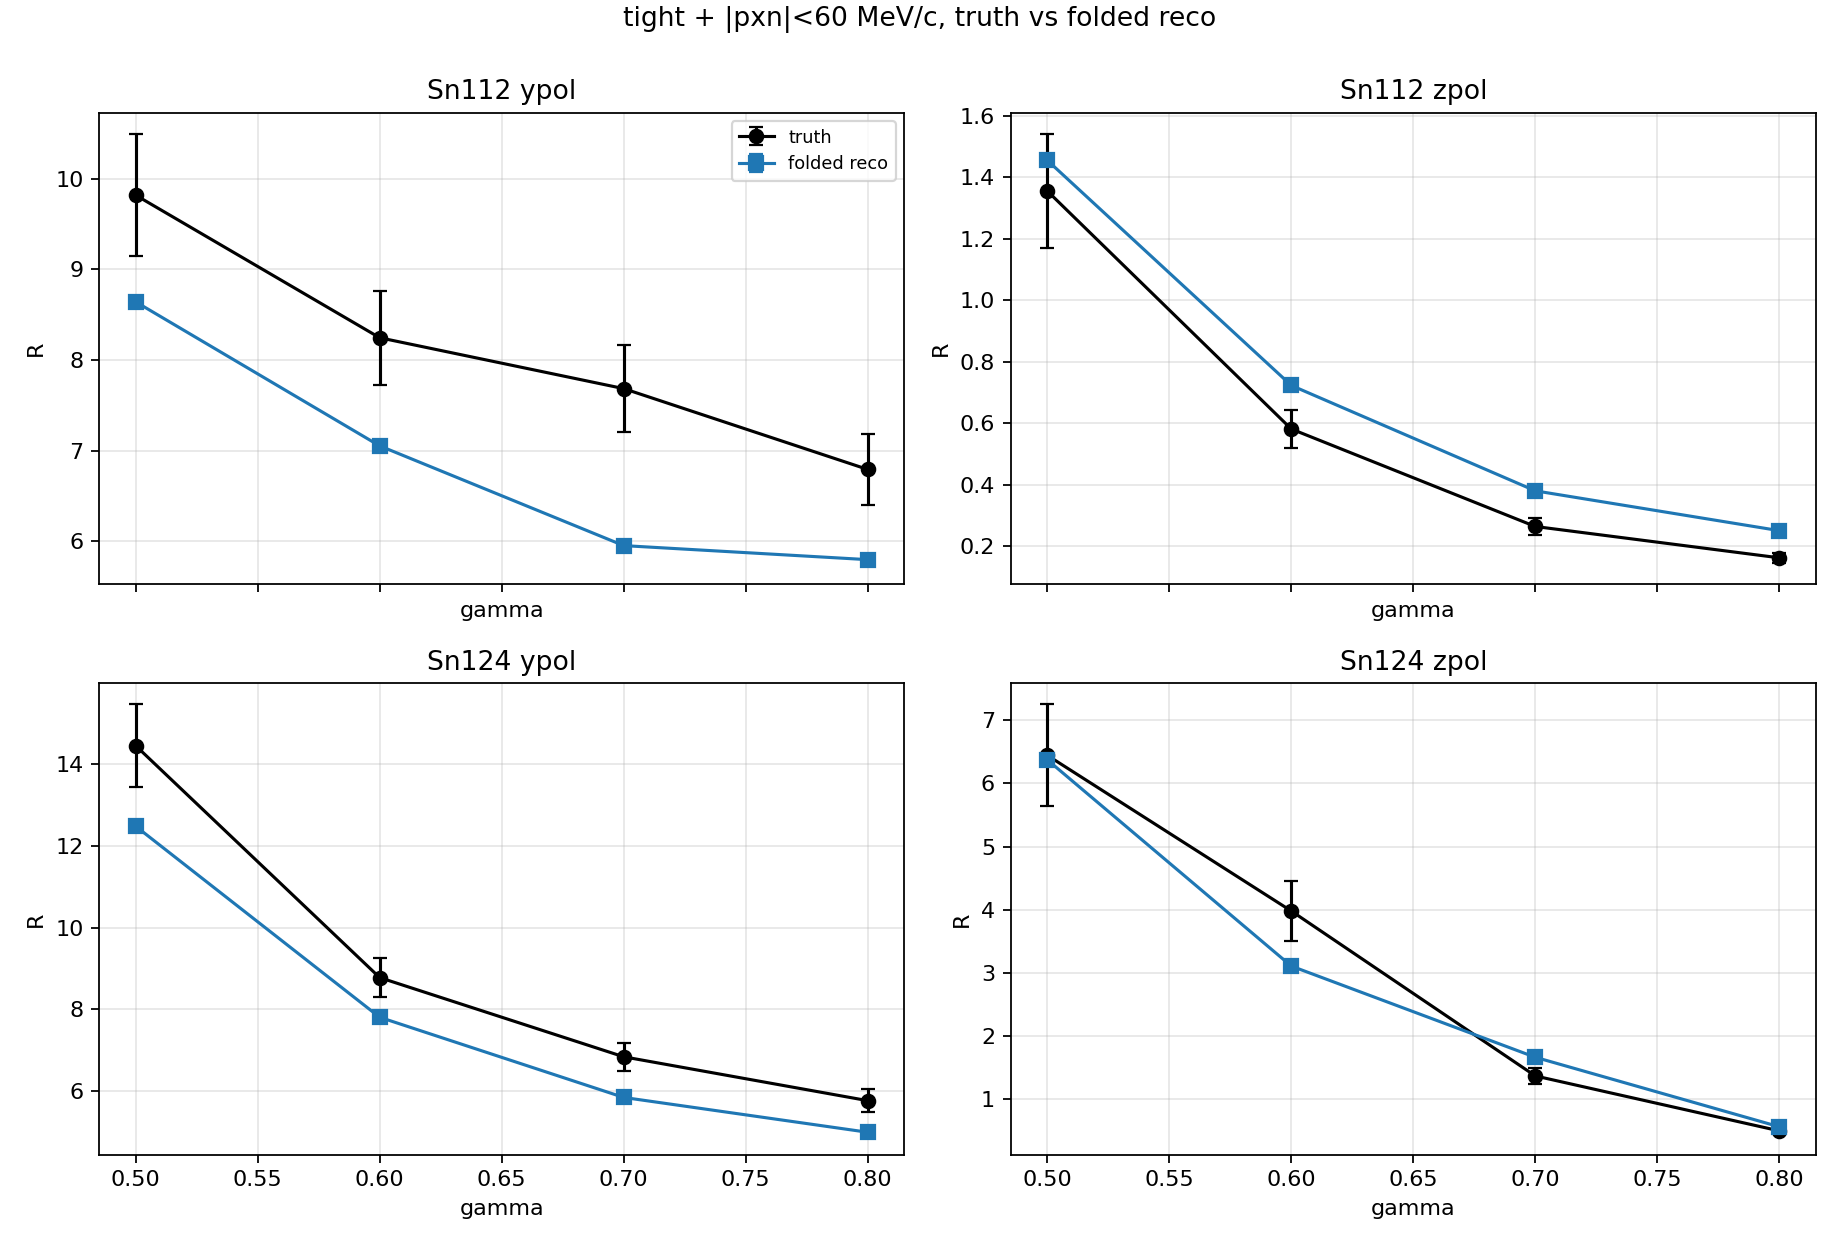
\includegraphics[width=\linewidth]{sn112_sn124_tight_px60_r_vs_gamma_expected_stat.png}
  \caption{Sn112/Sn124, tight, $|p_{x,n}|<60$ MeV/$c$ 的 truth 与 folded reco $R(\gamma)$。}
\end{figure}

Sn112/Sn124, \texttt{tight + |p\_x,n| < 60 MeV/c}, folded reco plane:

\begin{table}[H]
\centering
\begin{tabular}{lllrrrrr}
\toprule
target & pol & $\gamma$ & $N_{+}$ & $N_{-}$ & $R_{\mathrm{folded}}$ & $\sigma(R)_{\mathrm{sim}}$ & $\sigma(R)_{16\mathrm{h}}$ \\
\midrule
Sn112 & ypol & 0.5 & 1521 & 176 & 8.64 & 0.69 & 0.060 \\
Sn112 & ypol & 0.6 & 1629 & 231 & 7.05 & 0.50 & 0.045 \\
Sn112 & ypol & 0.7 & 1458 & 245 & 5.95 & 0.41 & 0.036 \\
Sn112 & ypol & 0.8 & 1478 & 255 & 5.80 & 0.39 & 0.035 \\
Sn112 & zpol & 0.5 & 80 & 55 & 1.45 & 0.25 & 0.0028 \\
Sn112 & zpol & 0.6 & 112 & 155 & 0.72 & 0.090 & 0.0014 \\
Sn112 & zpol & 0.7 & 95 & 250 & 0.38 & 0.046 & 0.0008 \\
Sn112 & zpol & 0.8 & 111 & 443 & 0.25 & 0.027 & 0.0006 \\
Sn124 & ypol & 0.5 & 2134 & 171 & 12.48 & 0.99 & 0.091 \\
Sn124 & ypol & 0.6 & 2147 & 275 & 7.81 & 0.50 & 0.047 \\
Sn124 & ypol & 0.7 & 2093 & 358 & 5.85 & 0.33 & 0.032 \\
Sn124 & ypol & 0.8 & 1948 & 390 & 4.99 & 0.28 & 0.026 \\
Sn124 & zpol & 0.5 & 306 & 48 & 6.38 & 0.99 & 0.014 \\
Sn124 & zpol & 0.6 & 208 & 67 & 3.10 & 0.44 & 0.005 \\
Sn124 & zpol & 0.7 & 214 & 129 & 1.66 & 0.18 & 0.0025 \\
Sn124 & zpol & 0.8 & 171 & 307 & 0.56 & 0.053 & 0.0008 \\
\bottomrule
\end{tabular}
\end{table}

$N_{+}$/$N_{-}$ 是 $\Delta p_x^{\mathrm{reco}}$ 正/负的事例数，$\sigma(R)_{\mathrm{sim}}$ 是当前 MC 样本的统计误差，$\sigma(R)_{16\mathrm{h}}$ 是外推到 16 h 束流时间后的统计误差 (公式见“统计量和束流时间”一节)。

这个图的重点不是 truth 和 reco 完全一致，而是 folded reco 曲线本身仍然随 $\gamma$ 单调变化，并且间隔远大于 16 h beamtime 下的统计误差。

\section{统计量和束流时间}

当前 beamtime planning anchor:
\begin{itemize}
  \item beam energy: 190 MeV/u
  \item beam intensity: $1.0\times 10^7$ pps
  \item SRC harmonic: 6
  \item bunch spacing: 33.62 ns
  \item planning breakup cross section: 550 mb
  \item planning detected-coincidence efficiency: 4.65\%
\end{itemize}

Sn124 1.2 g 库存下的 15 mm 圆盘:
\begin{itemize}
  \item 等效厚度: 0.929 mm
  \item detected coincidence rate: 843 Hz
  \item 16 h detected coincidences: $4.86\times 10^7$
\end{itemize}
Sn112 的 16 h usable 事件数在本节只使用同库存 atom-density scaling placeholder ($124/112$)，尚未替代为 Sn112 自己的 target-specific breakup cross section。

\subsection{QMD 样本量与通过率}

当前画图所用的 QMD 样本 (4 个 $\gamma$ 点求和) 在两个极化方向上极不均衡:

\begin{table}[H]
\centering
\begin{tabular}{llrrrrr}
\toprule
target & pol & $N_{\mathrm{raw}}$ (QMD) & $N_{\mathrm{tight}}$ & $N_{\mathrm{reco}}$(px60) & raw$\to$tight & raw$\to$reco \\
\midrule
Sn112 & ypol & $1.70\times10^6$ & $4.78\times10^4$ & $6.99\times10^3$ & 2.81\% & 0.411\% \\
Sn112 & zpol & $6.38\times10^4$ & $9.50\times10^3$ & $1.30\times10^3$ & 14.9\% & 2.04\% \\
Sn124 & ypol & $1.68\times10^6$ & $4.36\times10^4$ & $9.52\times10^3$ & 2.59\% & 0.566\% \\
Sn124 & zpol & $3.75\times10^4$ & $6.04\times10^3$ & $1.45\times10^3$ & 16.1\% & 3.87\% \\
\bottomrule
\end{tabular}
\end{table}

Sn124 的 zpol raw 样本最小，只有 $3.75\times10^4$ 个；Sn112 zpol 略大，为 $6.38\times10^4$ 个。$N_{\mathrm{reco}}$ 是当前 tight-px60 图实际使用的 usable $R$ 事件数。

把实验 16 h 的 expected usable 事件和当前 MC 画图统计直接对比:

\begin{table}[H]
\centering
\begin{tabular}{llrrrrr}
\toprule
target & pol & useful fraction & $N_{\mathrm{sim}}$ (当前图) & 16 h usable & 16 h $/$ $N_{\mathrm{sim}}$ & worst 3$\sigma$ $N_{\mathrm{req}}$ \\
\midrule
Sn112 & ypol & 0.00411 & $6.99\times10^3$ & $2.21\times10^5$ & $\sim$32$\times$ & $1.04\times10^5$ \\
Sn112 & zpol & 0.0204 & $1.30\times10^3$ & $1.10\times10^6$ & $\sim$840$\times$ & $2.93\times10^2$ \\
Sn124 & ypol & 0.00566 & $9.52\times10^3$ & $2.75\times10^5$ & $\sim$29$\times$ & $2.77\times10^3$ \\
Sn124 & zpol & 0.03869 & $1.45\times10^3$ & $1.88\times10^6$ & $\sim$1.3$\times10^3\times$ & $1.31\times10^2$ \\
\bottomrule
\end{tabular}
\end{table}

useful fraction $f_{\mathrm{useful}}=N_{\mathrm{reco}}/N_{\mathrm{raw}}$ 把 detected coincidences 折算到 usable $R$ 事件。Sn112 的 16 h usable 数值使用 $4.86\times10^7\times(124/112)\times f_{\mathrm{useful}}$；Sn124 使用 $4.86\times10^7\times f_{\mathrm{useful}}$。zpol 的实验统计增益尤其大；Sn112 ypol 的高 $\gamma$ 间隔统计裕量则明显更紧。

\subsection{统计误差推导}

$R=N_{+}/N_{-}$ 是比值统计量。在 $N=N_{+}+N_{-}$ 个有效事件的多项式模型下，用 delta method 给出
\[
  \sigma(R) = (1+R)\sqrt{R/N}.
\]
相邻两个 $\gamma$ 点 3$\sigma$ 区分所需事件数 (用两端均值 $\bar R=\tfrac12(R_1+R_2)$ 估 $\sigma$) 为
\[
  N_{\mathrm{req}} = \left[\, z_\alpha\,(1+\bar R)\sqrt{\bar R}\,/\,|\Delta R|\,\right]^2, \qquad z_\alpha=3.
\]
对应 tight px60 folded reco 的逐间隔结果:

\begin{table}[H]
\centering
\begin{tabular}{llrrrr}
\toprule
pol & 间隔 & $R_{\mathrm{left}}$ & $R_{\mathrm{right}}$ & $|\Delta R|$ & $N_{\mathrm{req}}(3\sigma)$ \\
\midrule
ypol & g050$\to$g060 & 12.48 & 7.81 & 4.67 & 519 \\
ypol & g060$\to$g070 & 7.81 & 5.85 & 1.96 & 979 \\
ypol & g070$\to$g080 & 5.85 & 4.99 & 0.85 & $2.77\times10^3$ \\
zpol & g050$\to$g060 & 6.38 & 3.10 & 3.27 & 131 \\
zpol & g060$\to$g070 & 3.10 & 1.66 & 1.45 & 117 \\
zpol & g070$\to$g080 & 1.66 & 0.56 & 1.10 & 36 \\
\bottomrule
\end{tabular}
\end{table}

Sn112 的同口径逐间隔结果为:

\begin{table}[H]
\centering
\begin{tabular}{llrrrr}
\toprule
pol & 间隔 & $R_{\mathrm{left}}$ & $R_{\mathrm{right}}$ & $|\Delta R|$ & $N_{\mathrm{req}}(3\sigma)$ \\
\midrule
ypol & g050$\to$g060 & 8.64 & 7.05 & 1.59 & $2.19\times10^3$ \\
ypol & g060$\to$g070 & 7.05 & 5.95 & 1.10 & $2.72\times10^3$ \\
ypol & g070$\to$g080 & 5.95 & 5.80 & 0.15 & $1.04\times10^5$ \\
zpol & g050$\to$g060 & 1.45 & 0.72 & 0.73 & 80 \\
zpol & g060$\to$g070 & 0.72 & 0.38 & 0.34 & 102 \\
zpol & g070$\to$g080 & 0.38 & 0.25 & 0.13 & 293 \\
\bottomrule
\end{tabular}
\end{table}

Sn124 最难区分的间隔是 ypol g070$\to$g080 ($\bar R=5.42$, $|\Delta R|=0.85$, 需 $2.77\times10^3$ 事件)；Sn112 最难区分的间隔也是 ypol g070$\to$g080 ($|\Delta R|=0.15$, 需 $1.04\times10^5$ 事件)。useful-event 外推链为
\[
  N_{\mathrm{usable}} = \mathrm{rate}\times T \times f_{\mathrm{useful}}, \qquad
  f_{\mathrm{useful}} = N_{\mathrm{reco\_plane}}(\mathrm{tight\,px60})/N_{\mathrm{raw}},
\]
Sn124 ypol $f_{\mathrm{useful}}=0.00566$ 给 $N_{\mathrm{usable}}=4.86\times10^7\times0.00566\approx2.75\times10^5$；Sn124 zpol $f_{\mathrm{useful}}=0.0387$ 给 $1.88\times10^6$。Sn112 在 atom-density scaling placeholder 下，ypol 为 $2.21\times10^5$，zpol 为 $1.10\times10^6$。

\subsection{统计 vs 系统对照}

把 ypol tight px60 的三个量级放在一起:

\begin{table}[H]
\centering
\begin{tabular}{lr}
\toprule
量 & 典型值 \\
\midrule
$\sigma_{\mathrm{stat}}(R)$ @ 16 h (每个 $\gamma$ 点) & 0.026 -- 0.091 \\
$\Delta R_{\mathrm{detector}}$ (truth$\to$reco, 每个 $\gamma$ 点) & 1 -- 2 \\
$\Delta R_{\mathrm{between}\,\gamma}$ (最难间隔 g070$\to$g080) & 0.85 \\
\bottomrule
\end{tabular}
\end{table}

16 h 统计误差 ($\sim$0.03--0.09) 比探测器 folding 造成的 $R$ 偏移 ($\sim$1--2) 小一到两个量级，比最小 $\gamma$ 间距 (0.85) 也小约一个量级。因此 ``统计不是瓶颈、系统主导'' 这一结论有定量支撑。

\begin{figure}[H]
  \centering
 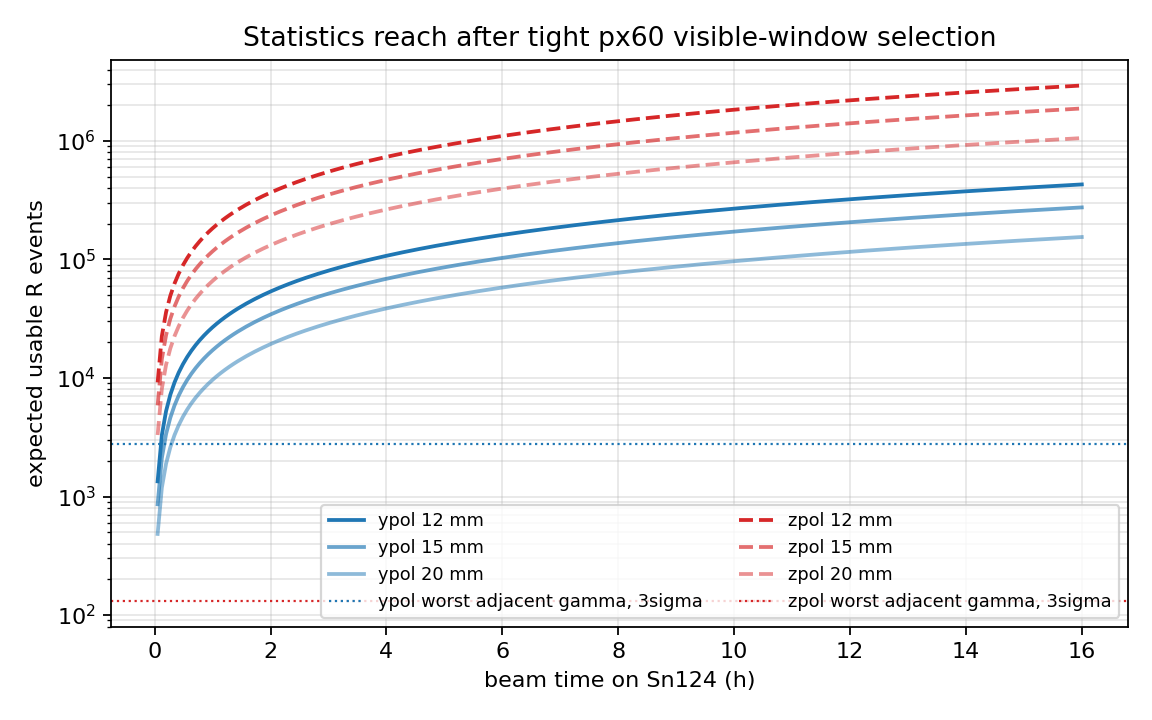
\includegraphics[width=0.9\linewidth]{sn124_beamtime_reach_tight_px60.png}
  \caption{Sn124 库存靶方案下，tight px60 visible-window selection 后的 usable $R$ event reach。}
\end{figure}

\begin{figure}[H]
  \centering
  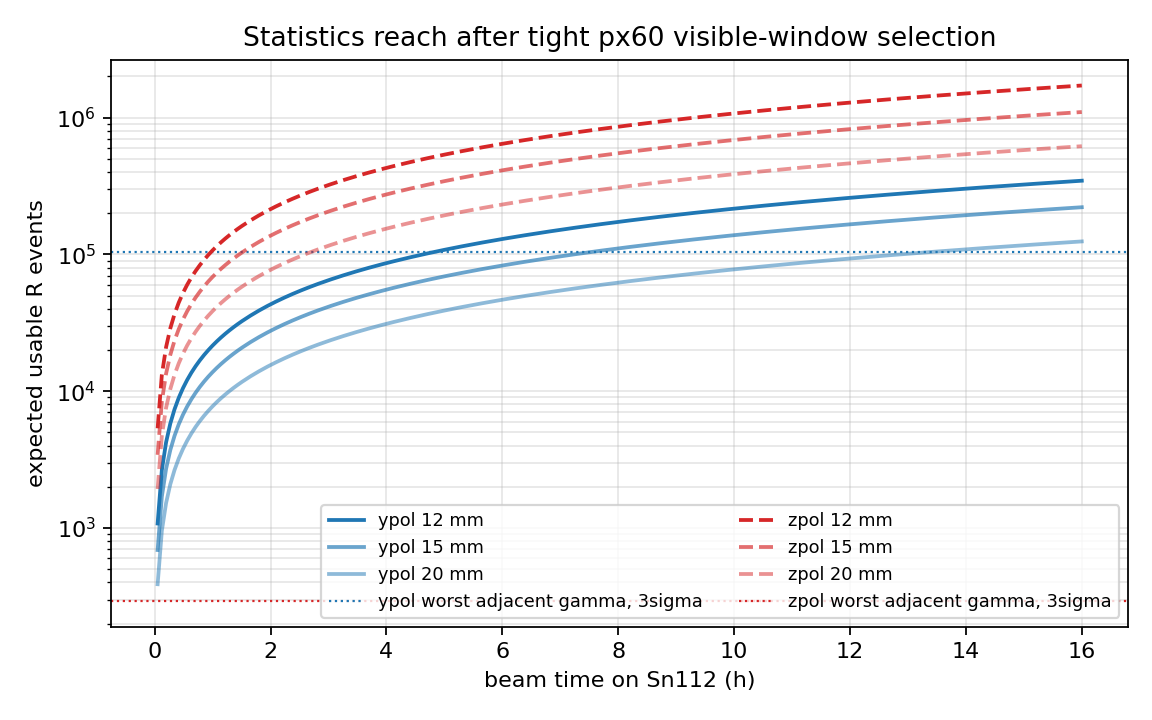
\includegraphics[width=0.9\linewidth]{sn112_beamtime_reach_tight_px60.png}
  \caption{Sn112 库存靶方案下，tight px60 visible-window selection 后的 usable $R$ event reach；rate 使用 atom-density scaling placeholder。}
\end{figure}

即使采用 20 mm 圆盘、同样 1.2 g 库存，16 h 后 Sn124 和 Sn112 ypol usable $R$ events 都在 $10^5$ 量级以上。Sn124 的相邻 $\gamma$ 统计裕量很大；Sn112 ypol 的 $g070\to g080$ 间隔较窄，统计裕量只有约 $2.1\times$，因此更依赖 detector/model folding 的系统控制。

pile-up 方面，旧 planning 的 3 mm reference thickness 下每 bucket detected coincidence mean 约 $9.16\times 10^{-5}$。15 mm 库存方案 rate 更低，因此 single-bucket pile-up 不是当前主瓶颈。仍需检查电子学积分窗是否跨多个 bucket。

\section{建议的 gamma 约束流程}

推荐主线如下:
\begin{enumerate}
  \item 对每个 $\gamma$ 的 QMD 输出，跑同一套 Geant4 几何、NEBULA-Plus detector response、PDC NN proton reconstruction、neutron reconstruction。
  \item 用同一 selection 定义实验和模型的 folded observable: $|p_{x,n}^{\mathrm{reco}}| < 60$ MeV/$c$，并使用 tight event selection；Sn124 作为主锚点，Sn112 作为独立同位素通道交叉检查。
  \item 对实验数据构造
  \[
    R_{\mathrm{exp}}
    =
    \frac{N(\Delta p_x^{\mathrm{reco}}>0)}
         {N(\Delta p_x^{\mathrm{reco}}<0)}.
  \]
  \item 对模型构造 $R_{\mathrm{model,folded}}(\gamma)$。
  \item 用 likelihood 或 $\chi^2$ 做约束:
  \[
    \chi^2(\gamma)
    =
    \frac{
      \left[
        R_{\mathrm{exp}} - R_{\mathrm{model,folded}}(\gamma)
      \right]^2
    }{
      \sigma_{\mathrm{stat}}^2
      + \sigma_{\mathrm{detector}}^2
      + \sigma_{\mathrm{model}}^2
    }.
  \]
  \item 组合 ypol/zpol 和 Sn112/Sn124 时，要先确认每个通道的 folding closure 和系统误差，不要只按统计误差合并。
\end{enumerate}

这一路线的优点是避免不稳定 unfolding。只有在 closure test 证明 response matrix 可逆、效率没有近零区域主导时，再把 unfolded truth-level $R$ 作为附加结果。

\section{Detector folding 技术诊断}

这里要回答的问题不是 ``reco $R$ 是否等于 truth $R$''，而是 reco $R$ 是否是一个可建模、可闭合检验的 folded observable。当前 diagnostics 把 folding 拆成 event selection、neutron visible-window efficiency、reconstruction response、reaction-plane migration 和最终 $R$ ladder。当前输出还没有独立的逐层 proton detector efficiency 表；proton/PDC 对反应平面的影响通过 reconstructed event plane、response matrix，以及 $R$ ladder 中 \texttt{reco\_truth\_plane} 到 \texttt{reco\_plane} 的变化来评估。

\subsection{event selection 和 visible-window survival}

\begin{figure}[H]
  \centering
  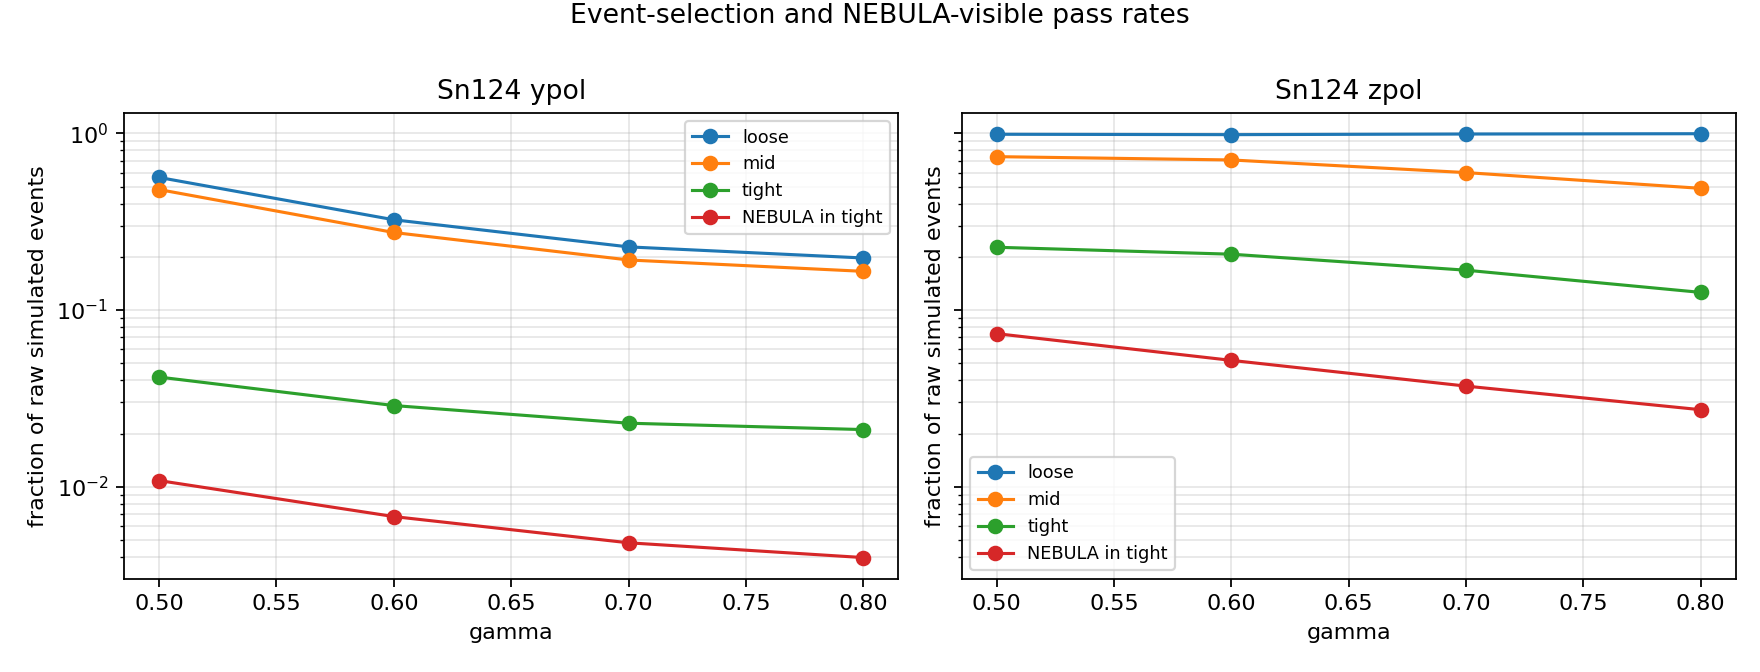
\includegraphics[width=0.96\linewidth]{sn124_selection_passrates.png}
  \caption{Sn124 selection pass rate 随 $\gamma$ 的变化。最后进入 folded $R$ 的是 tight 且 NEBULA-visible 的小分支。}
\end{figure}

Sn124 pooled ypol 的 raw-to-tight 和 raw-to-NEBULA-visible 比例约为 $2.59\%$ 和 $0.571\%$；zpol 约为 $16.1\%$ 和 $3.93\%$。这些数值只作为当前 full simulation 给出的 usable-event survival，不等同于实验中的 coincidence efficiency calibration。

\begin{figure}[H]
  \centering
  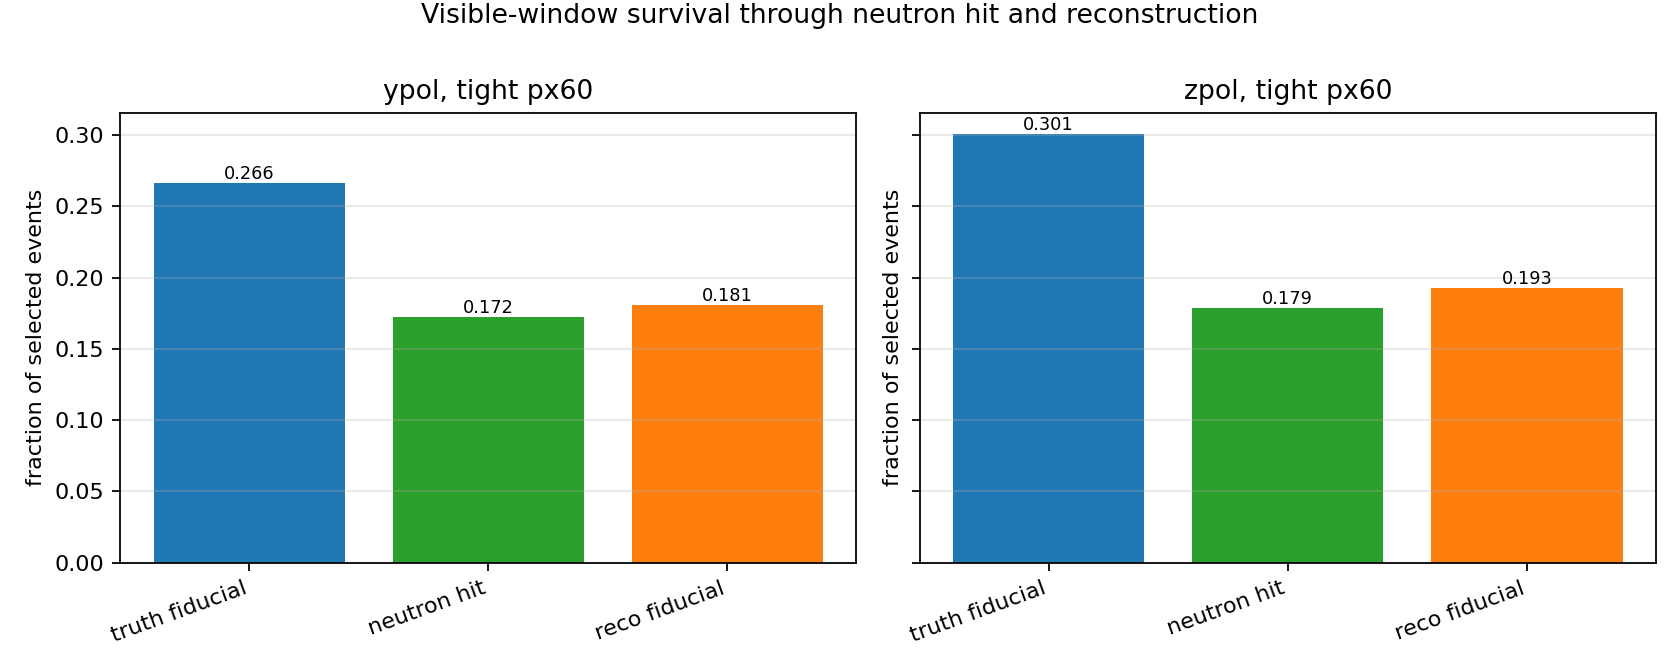
\includegraphics[width=0.95\linewidth]{survival_flow_tight_px60.png}
  \caption{tight px60 diagnostic sample 内的 survival flow。truth fiducial 由 visible-window 定义决定，后续两步分别看 neutron hit 和 reconstructed-fiducial survival。}
\end{figure}

pooled tight px60 中，ypol 从 selected events 到 truth fiducial、neutron hit、reco fiducial 的比例分别是 $0.266$、$0.172$、$0.181$；zpol 分别是 $0.301$、$0.179$、$0.193$。reco fiducial 略高于 hit truth fiducial 是因为 fiducial 条件在重建后定义，存在边界迁移。

\subsection{neutron efficiency 的 px-py 和 Delta-px 相空间}

\begin{figure}[H]
  \centering
  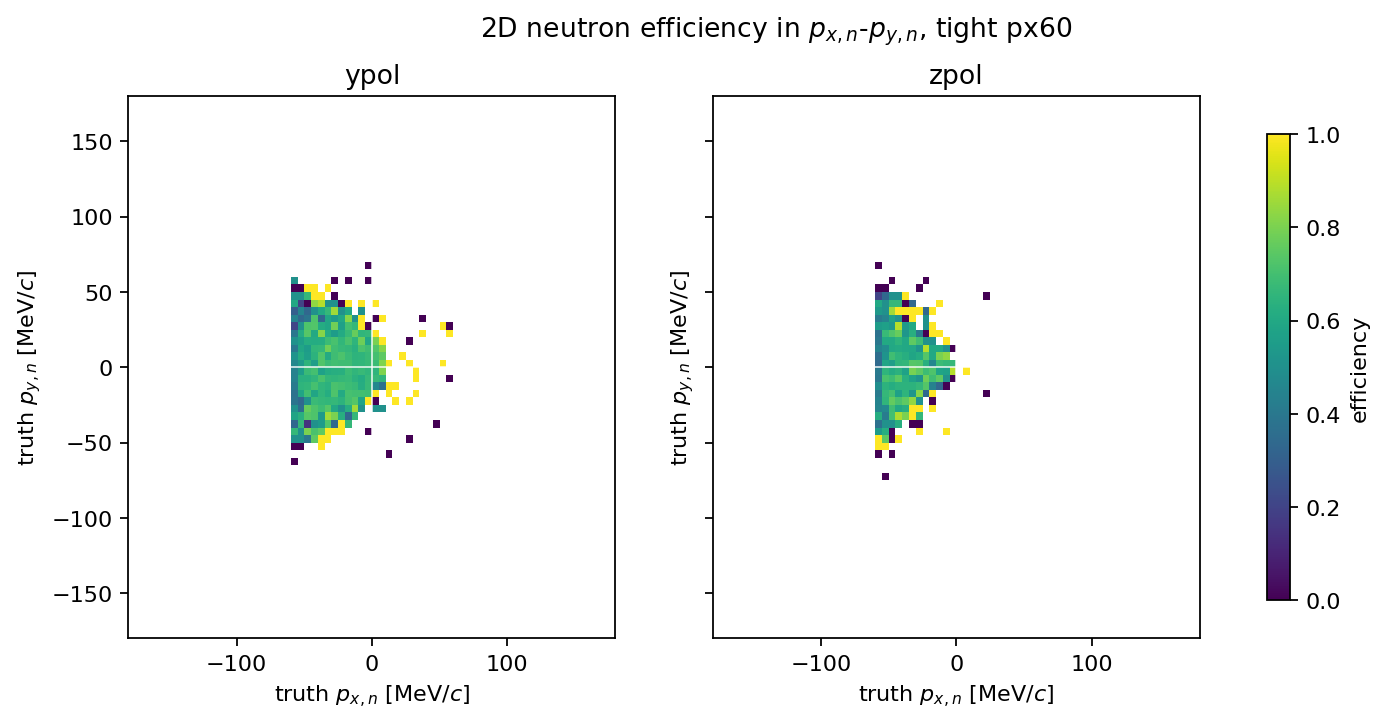
\includegraphics[width=0.96\linewidth]{neutron_efficiency_2d_pxn_vs_pyn_tight_px60.png}
  \caption{tight px60 下 truth $p_{x,n}$ 与 truth $p_{y,n}$ 的二维 neutron efficiency。白色区域是当前 diagnostic 中没有可用统计的相空间。}
\end{figure}

\begin{figure}[H]
  \centering
  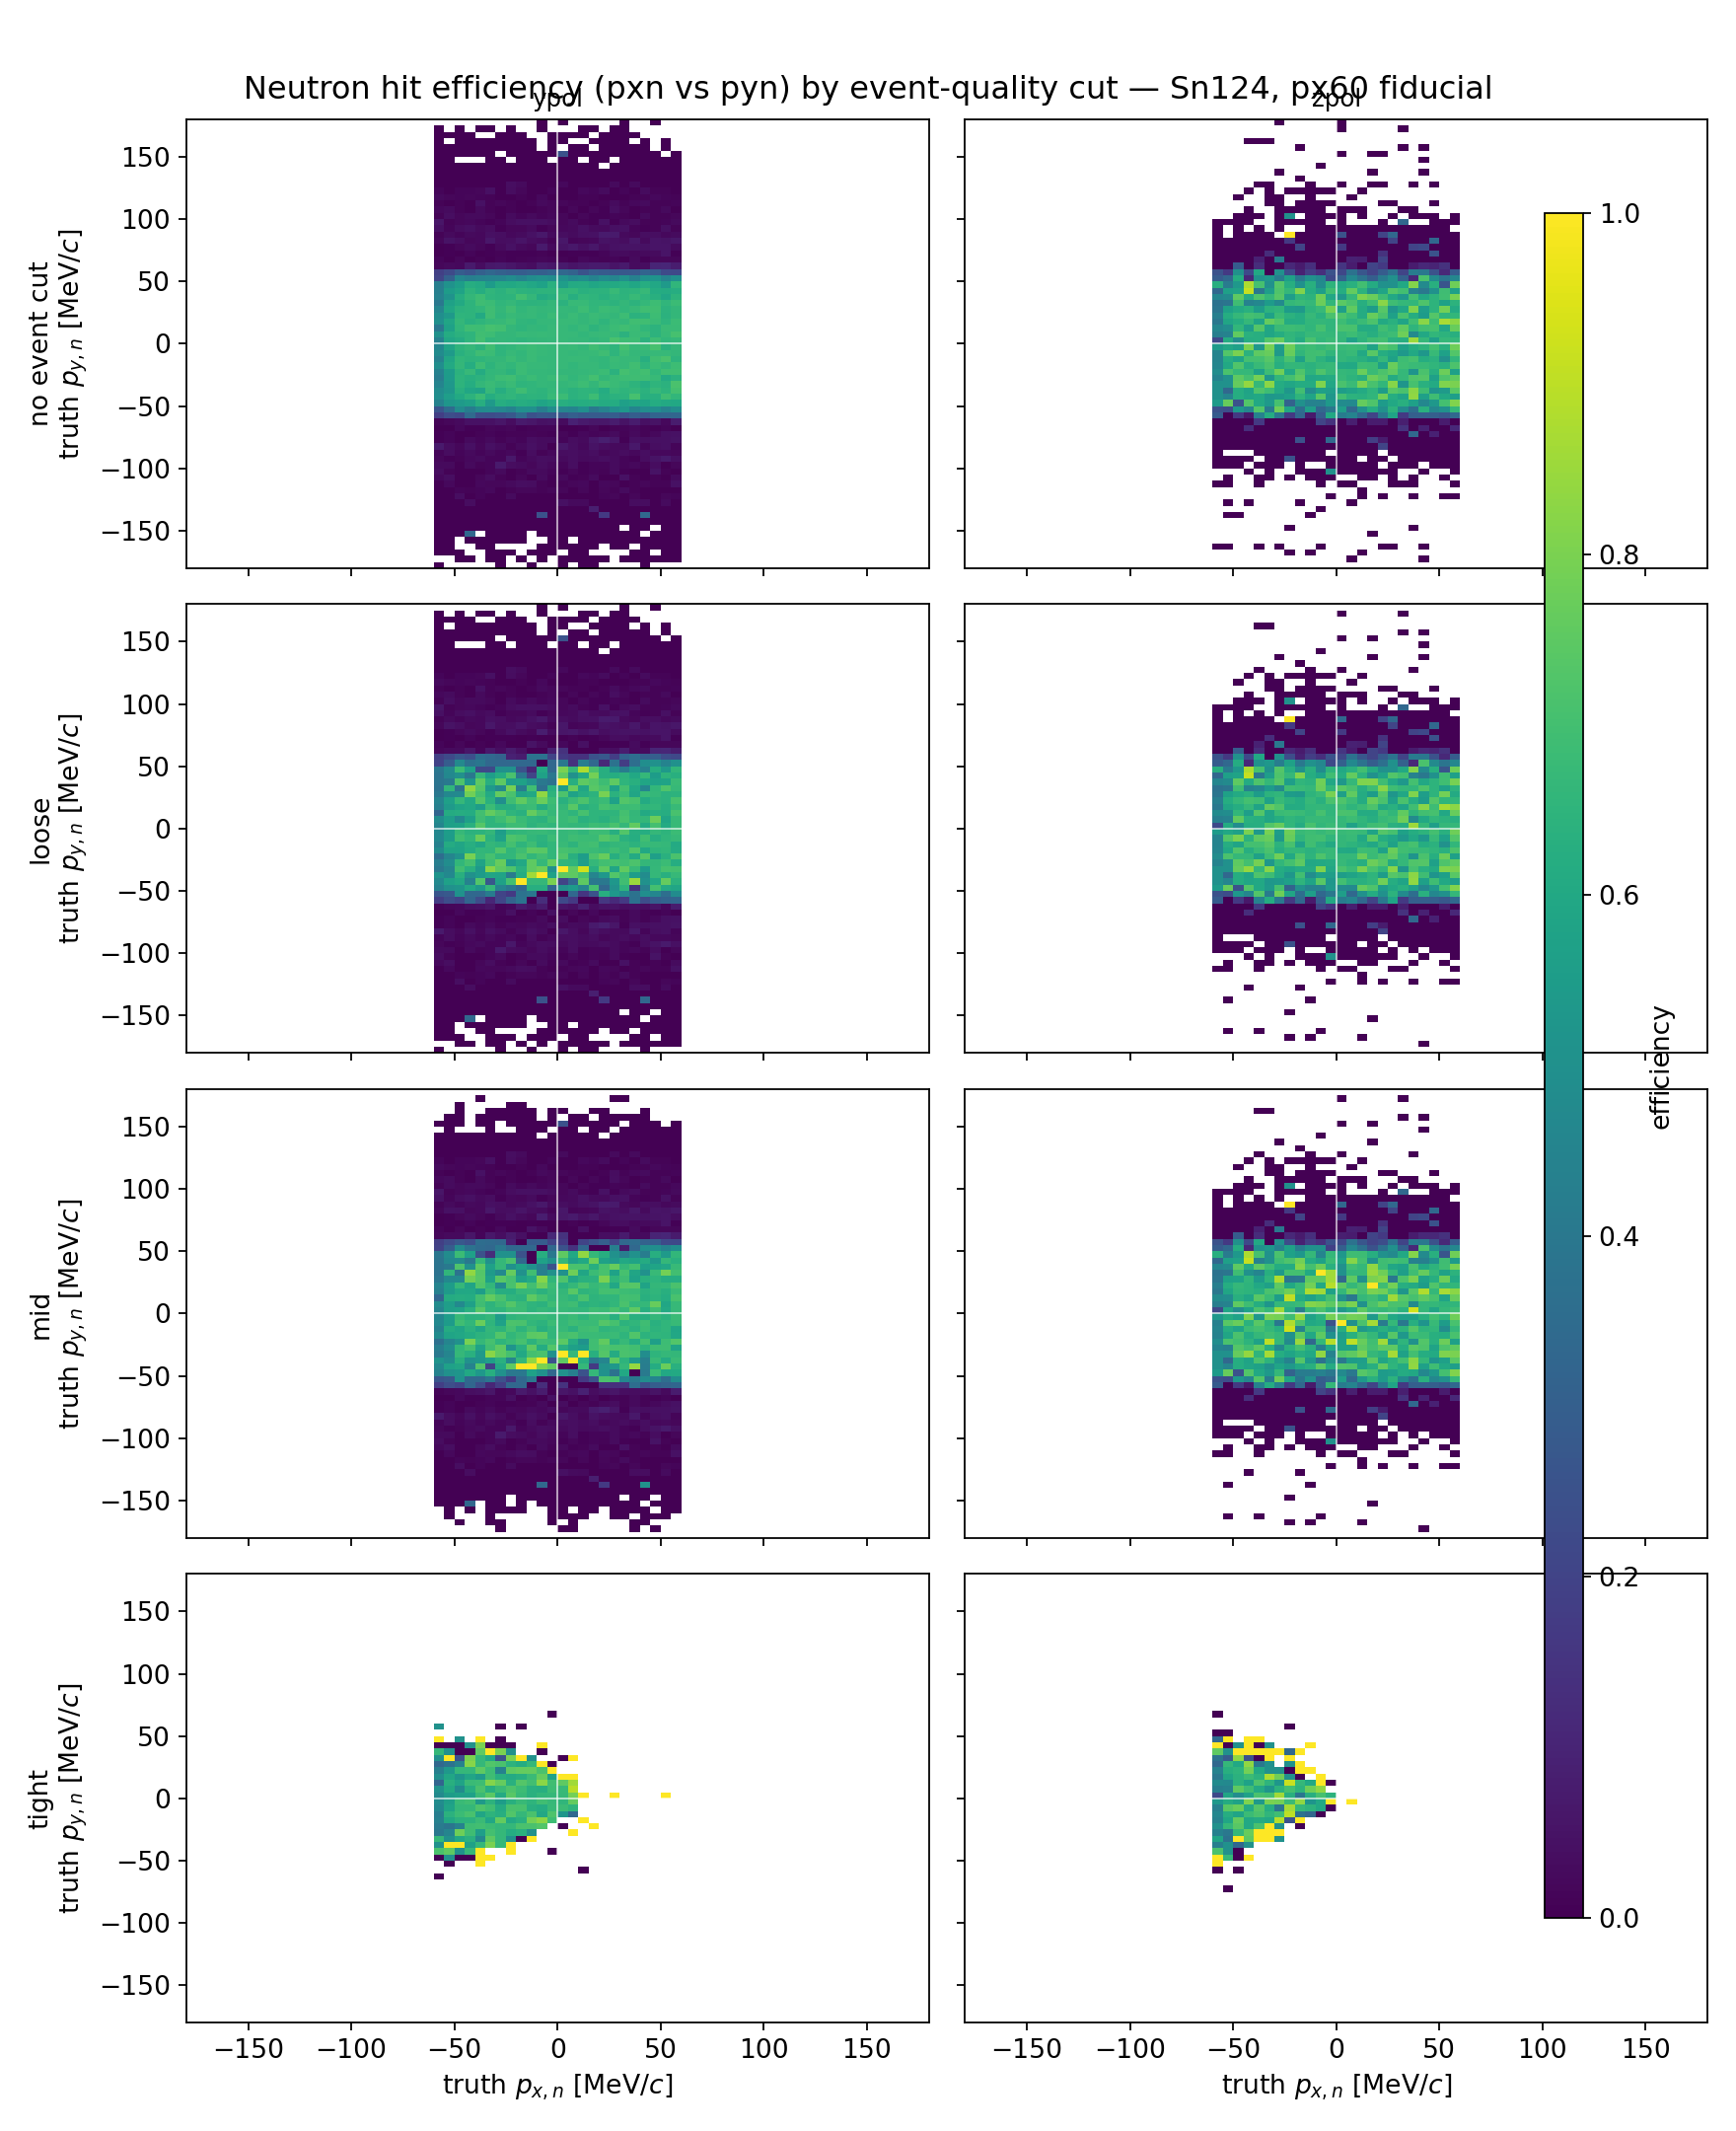
\includegraphics[width=0.82\linewidth]{cut_diagnostics/neutron_efficiency_2d_pxn_vs_pyn_by_cut.png}
  \caption{同一 $p_{x,n}$--$p_{y,n}$ 效率图，但按 event-quality cut 分行 (none/loose/mid/tight)，列为 ypol/zpol (全部 px60 truth fiducial)。从 none 到 tight，高效率区的形状基本不变，说明 cut 改变的是采样的相空间区域而非单 bin 效率。}
\end{figure}

\begin{figure}[H]
  \centering
  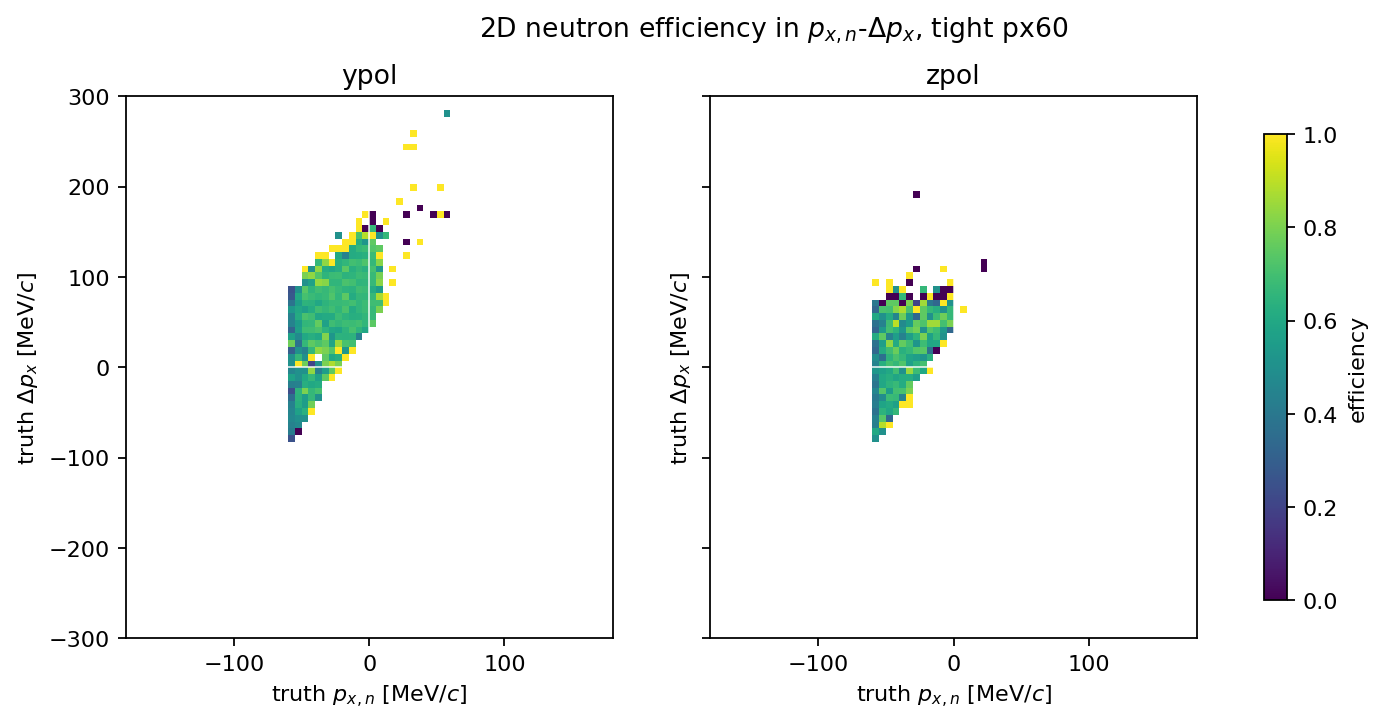
\includegraphics[width=0.96\linewidth]{neutron_efficiency_2d_pxn_vs_dpx_tight_px60.png}
  \caption{tight px60 下 truth $p_{x,n}$ 与 truth $\Delta p_x$ 的二维 neutron efficiency。这张图直接说明 neutron acceptance 如何进入 $R$ 的 numerator/denominator。}
\end{figure}

\begin{figure}[H]
  \centering
  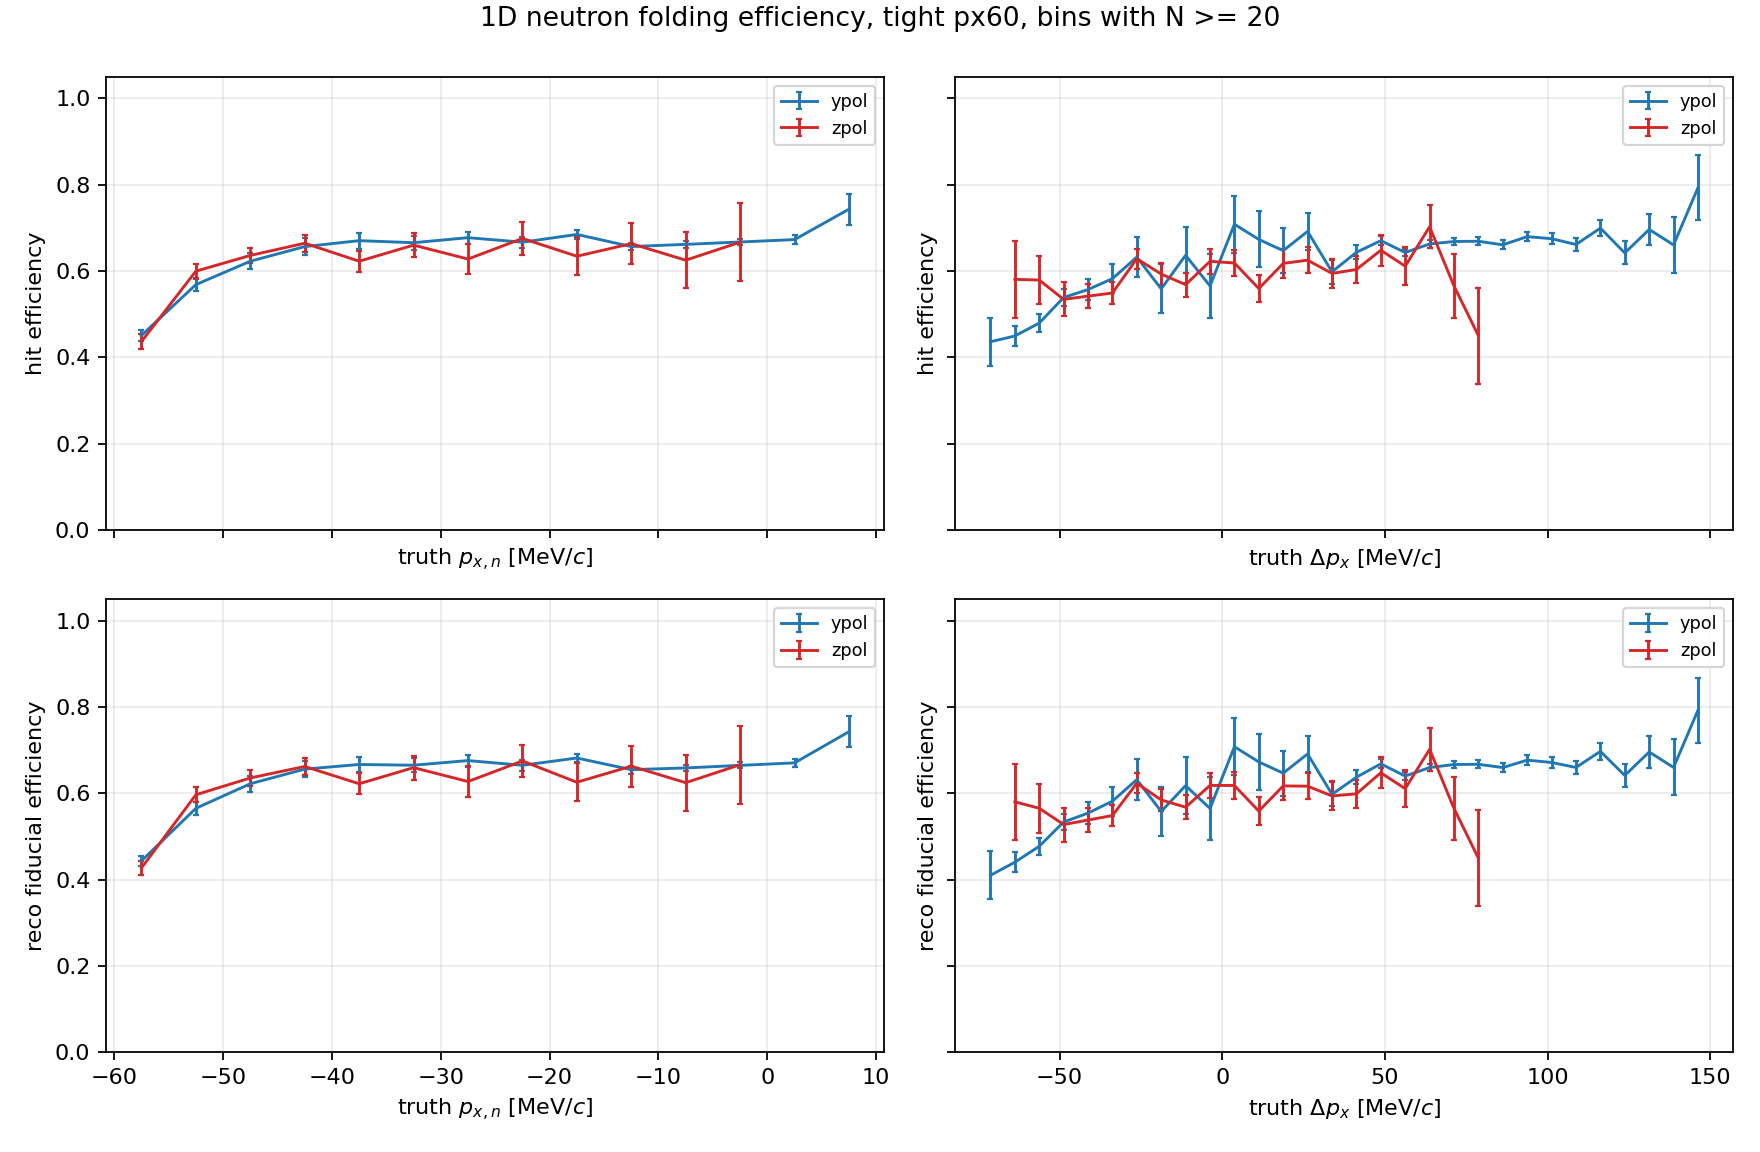
\includegraphics[width=0.96\linewidth]{neutron_efficiency_1d_tight_px60.png}
  \caption{至少有 20 个 truth events 的 bin 中，一维 neutron hit 和 reco fiducial efficiency。在 populated core 中，efficiency 大约为 0.55--0.70，并不是 1。}
\end{figure}

visible sample 不是 breakup phase space 的均匀切片。tight px60 的主要 populated 区域在负 $p_{x,n}$，efficiency 同时随 $p_{x,n}$ 和 $\Delta p_x$ 变化。因此 proposal 里不应说实验直接测到了 truth-level $R$；更稳的说法是: 每个理论 $\gamma$ 点都用同一套 efficiency/response folding，再和实验 folded observable 比较。

\subsection{sign-dependent neutron efficiency 和 px60 选择}

\begin{figure}[H]
  \centering
  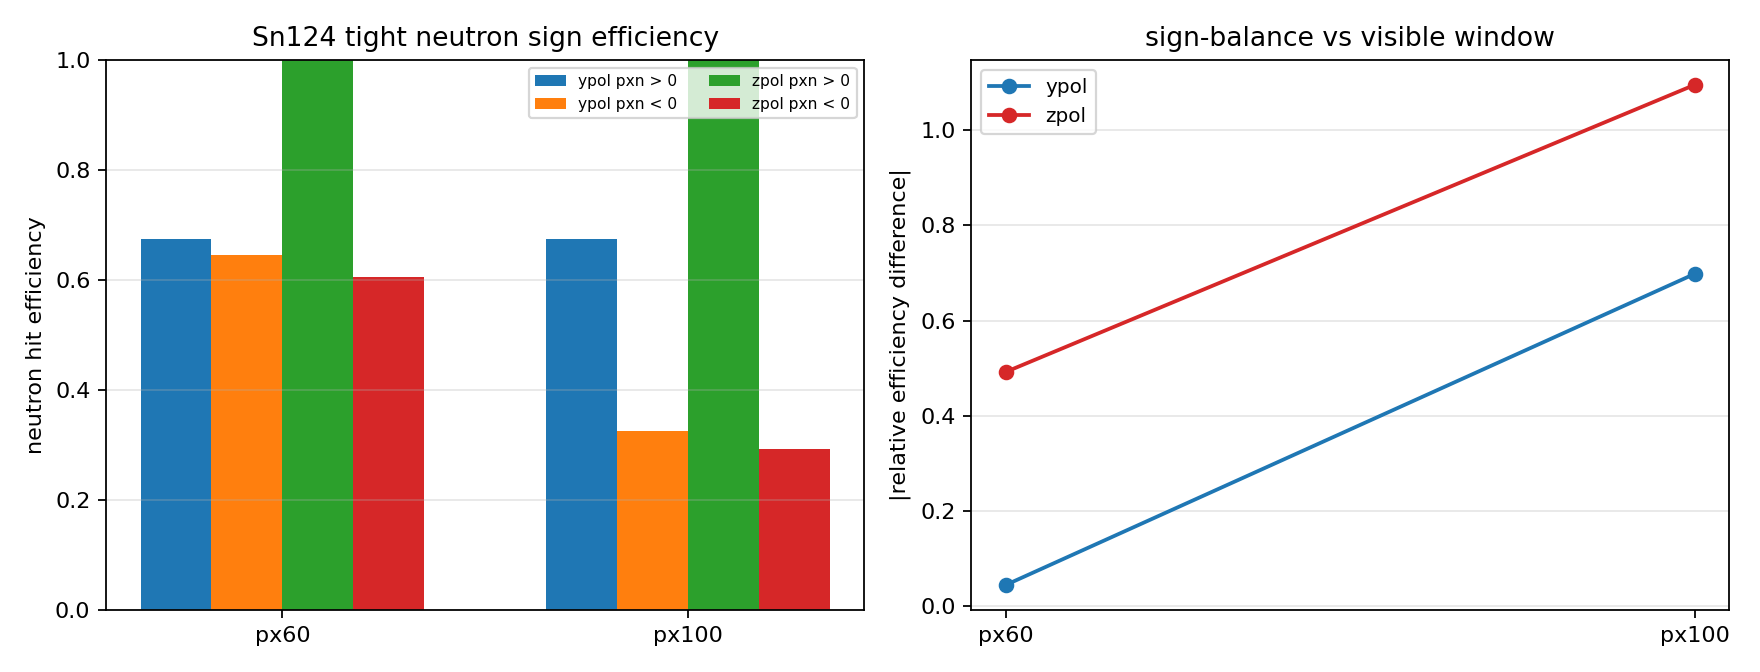
\includegraphics[width=0.95\linewidth]{ypol_tight_neutron_efficiency_balance.png}
  \caption{tight selection 下的 neutron sign efficiency balance。ypol 给出稳定的 sign-balance 对比；zpol tight 的正 $p_{x,n}$ 分支在当前 MC diagnostic 中统计太少。}
\end{figure}

ypol tight 的 neutron hit efficiency:

\begin{table}[H]
\centering
\begin{tabular}{lrrr}
\toprule
fiducial & $\epsilon(p_{x,n}>0)$ & $\epsilon(p_{x,n}<0)$ & relative difference \\
\midrule
px60 & 0.678 & 0.644 & 0.050 \\
px100 & 0.677 & 0.293 & 0.791 \\
\bottomrule
\end{tabular}
\end{table}

\texttt{px100} 会保留一个 NEBULA 很难看到的负 $p_{x,n}$ 分支，导致 $R$ 被 detector efficiency 强烈扭曲。\texttt{px60} 不是消除所有 detector effect，而是把 ypol 中最严重的 sign-dependent efficiency 降到可建模、可做 closure test 的范围。当前 zpol tight 的 sign-balance 数值不能过度解释，因为正 $p_{x,n}$ 分支在该 diagnostic 表里只有 3 个事件。

\subsection{momentum response 和 reaction-plane response}

\begin{figure}[H]
  \centering
  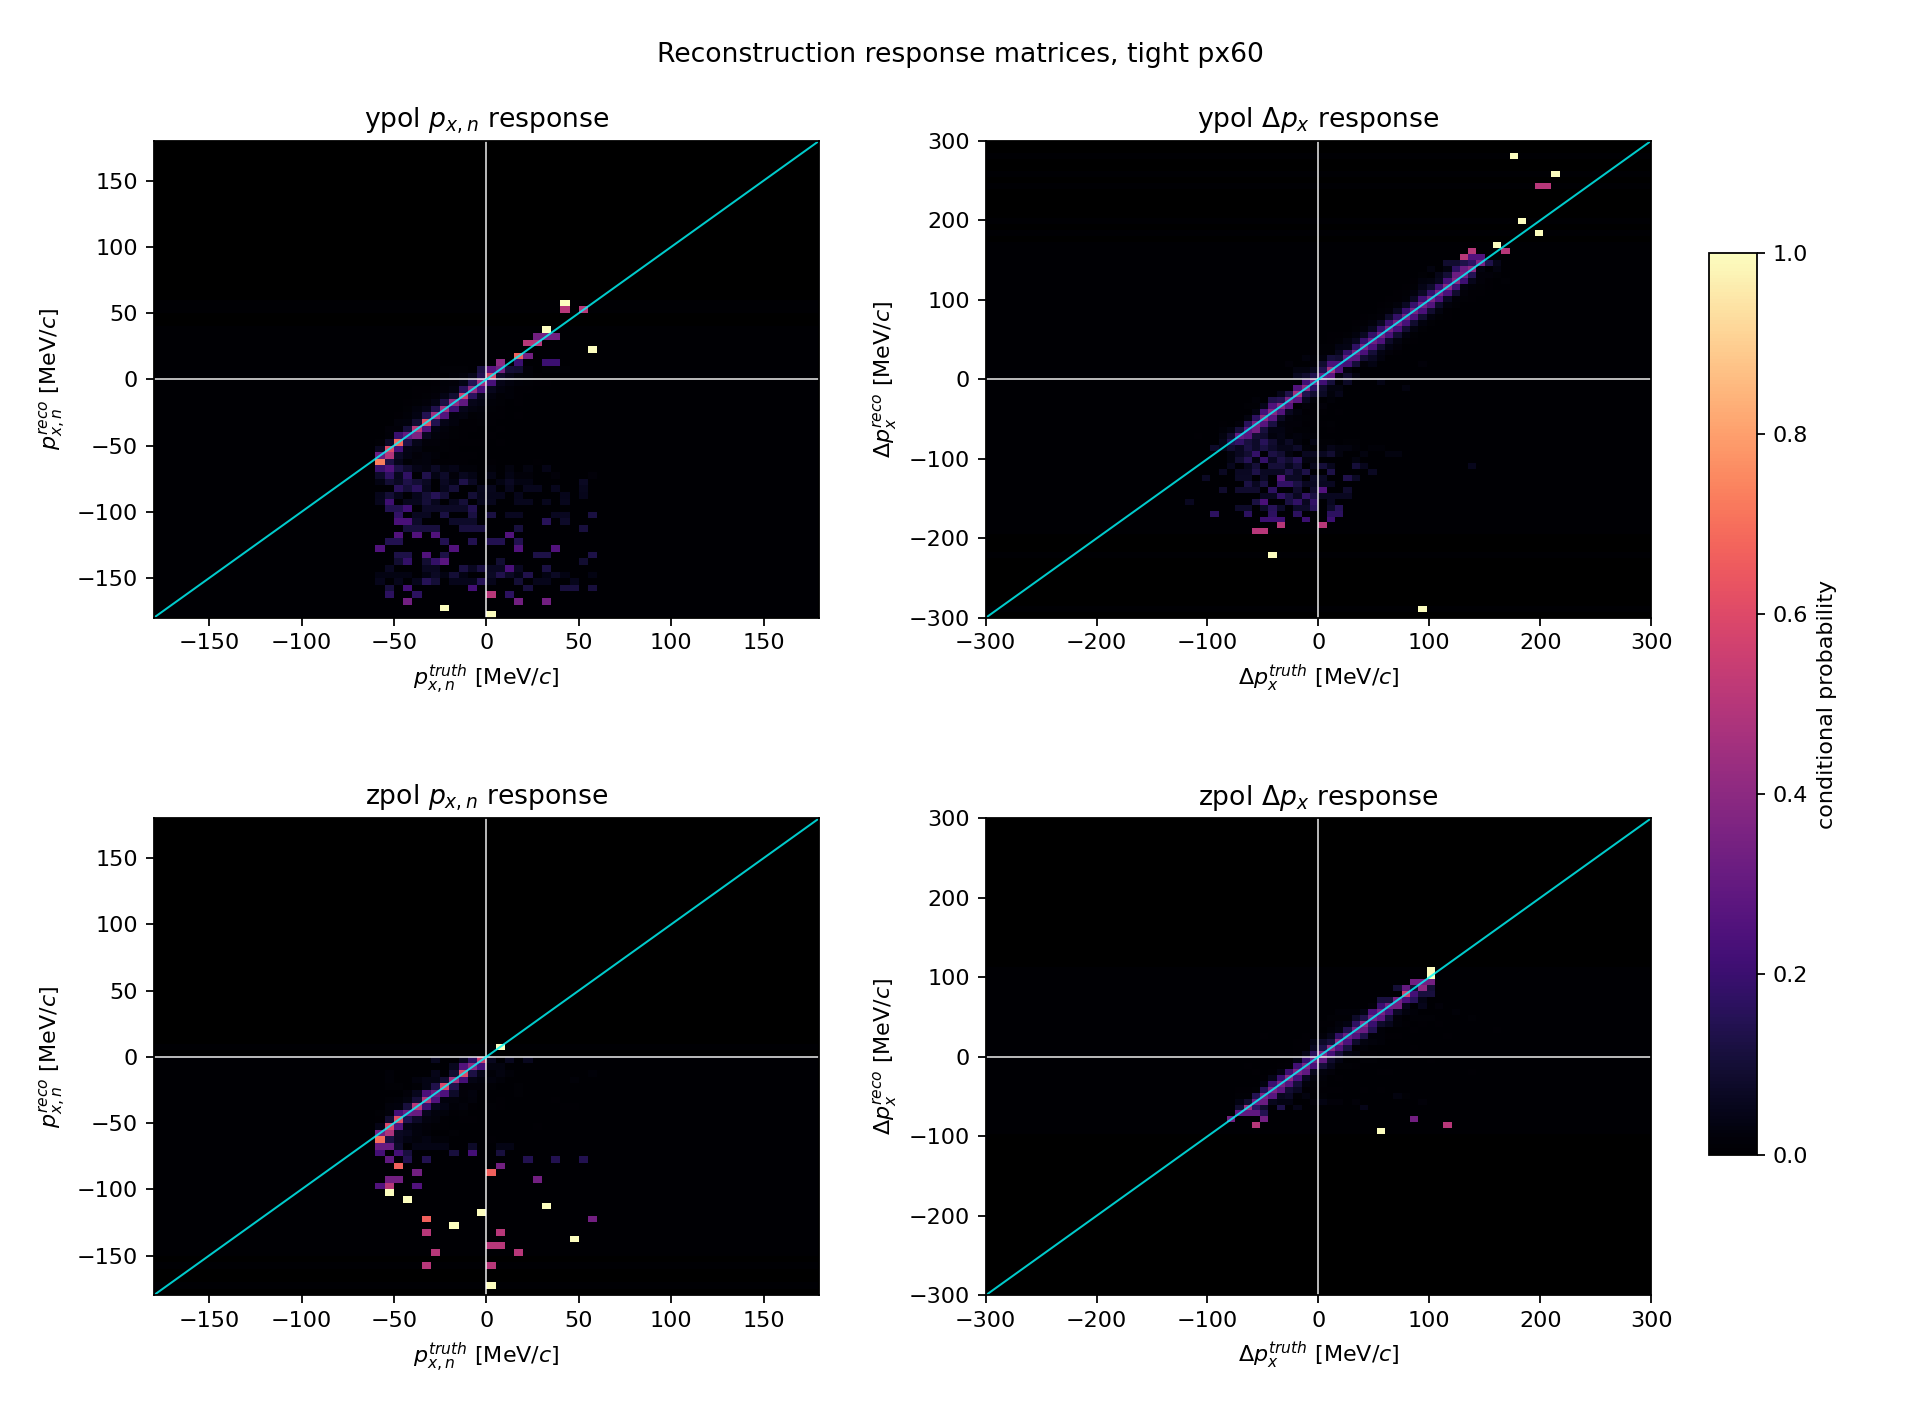
\includegraphics[width=0.96\linewidth]{response_matrices_tight_px60.png}
  \caption{tight px60 下 reconstructed $p_{x,n}$ 和 reconstructed $\Delta p_x$ 的 conditional response matrix。青色线是对角线；黑色区域是没有可用 diagnostic 统计的 bin。}
\end{figure}

核心相空间中，$\Delta p_x$ response 在 ypol/zpol 都接近对角线；$p_{x,n}$ response 在接受分支较窄，但有低概率尾巴和边界效应。这说明 smearing 需要 folding，但一阶偏置主要仍来自 neutron visible-window selection。

\begin{figure}[H]
  \centering
  \begin{minipage}{0.48\linewidth}
    \centering
    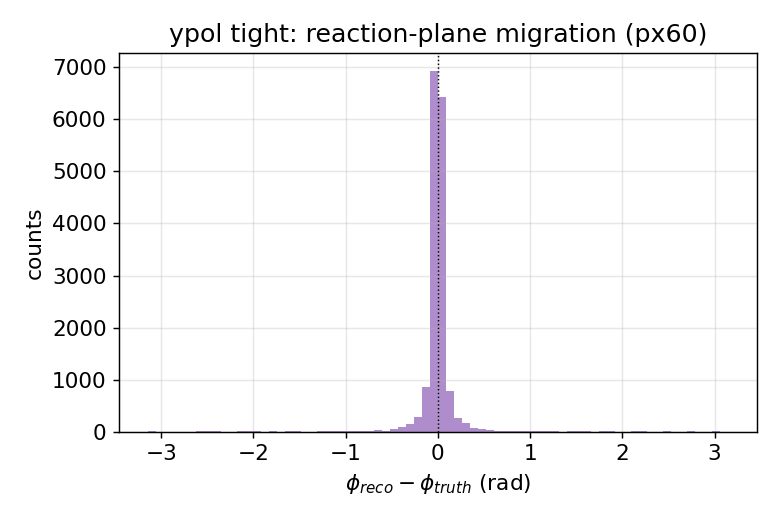
\includegraphics[width=\linewidth]{dphi_reco_truth_ypol_tight_px60.png}
  \end{minipage}
  \hfill
  \begin{minipage}{0.48\linewidth}
    \centering
    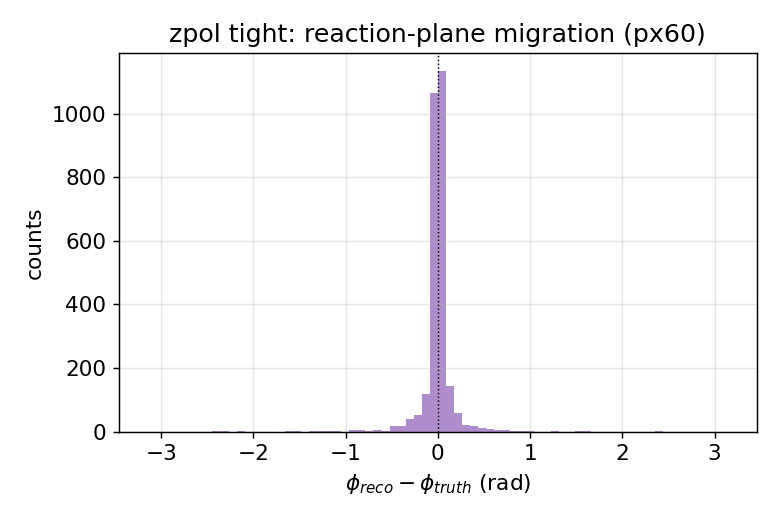
\includegraphics[width=\linewidth]{dphi_reco_truth_zpol_tight_px60.png}
  \end{minipage}
  \caption{ypol/zpol tight px60 的 reconstructed minus truth reaction-plane angle。这是 proton/PDC 驱动的 event-plane reconstruction 对 $R$ 的直接诊断。}
\end{figure}

\subsection{folding 在哪里改变 R}

\begin{figure}[H]
  \centering
  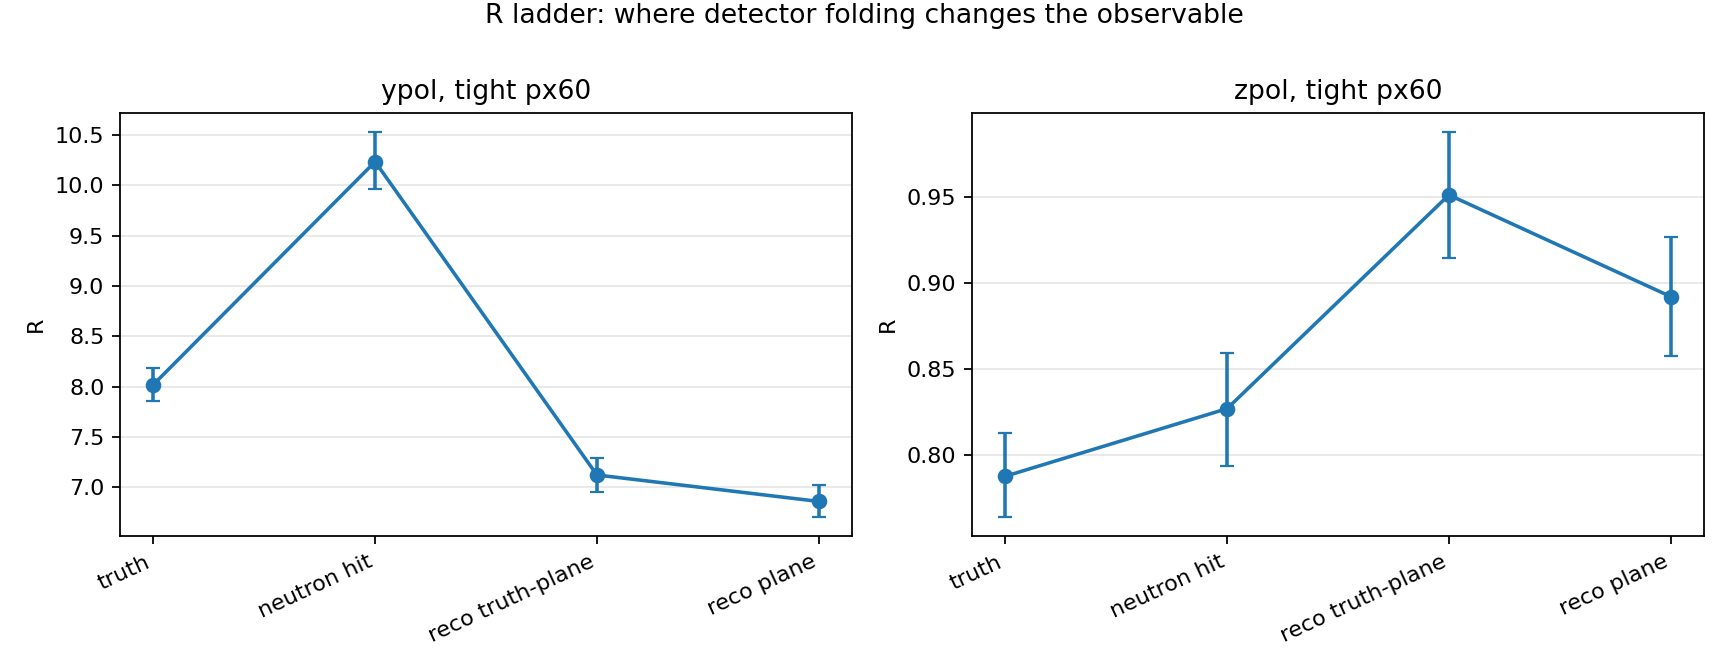
\includegraphics[width=0.96\linewidth]{r_ladder_summary_tight_px60.png}
  \caption{ypol/zpol tight px60 的 $R$ ladder。该图把 truth、neutron hit acceptance、truth-plane reconstruction、fully reconstructed event plane 分开。}
\end{figure}

pooled ypol tight px60:

\begin{table}[H]
\centering
\begin{tabular}{lrrrr}
\toprule
stage & $N$ & $N_{\mathrm{pos}}$ & $N_{\mathrm{neg}}$ & $R$ \\
\midrule
truth & 24323 & 21626 & 2697 & 8.02 \\
hit\_truth & 15751 & 14349 & 1402 & 10.23 \\
reco\_truth\_plane & 16509 & 14476 & 2033 & 7.12 \\
reco\_plane & 16509 & 14408 & 2101 & 6.86 \\
\bottomrule
\end{tabular}
\end{table}

最大的变化发生在最终 event-plane reconstruction 之前: neutron hit acceptance 和 reconstructed visible-window definition 已经显著改变 observable。\texttt{reco\_truth\_plane} 到 \texttt{reco\_plane} 的变化较小，说明当前样本中 PDC/reaction-plane reconstruction 不是 $R$ bias 的主导项。

\subsection{sign migration 不是主导项}

\begin{figure}[H]
  \centering
  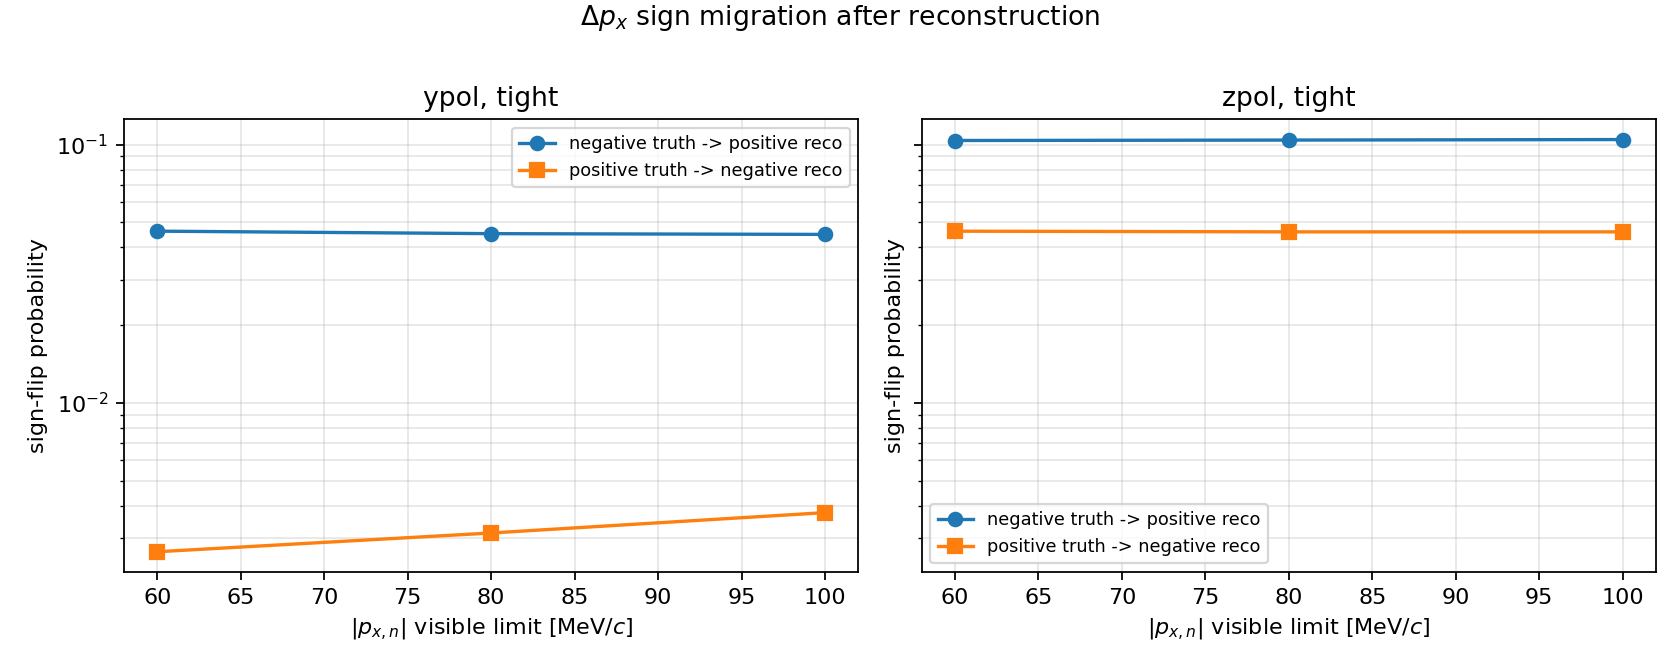
\includegraphics[width=0.95\linewidth]{sign_migration_summary_tight.png}
  \caption{tight selection 下 $\Delta p_x$ sign-flip probability 随 neutron visible-window size 的变化。sign migration 定义为条件概率 $P(\mathrm{reco\ sign}\,|\,\mathrm{truth\ sign})$，其中 truth sign $=\mathrm{sgn}(\Delta p_x^{\mathrm{truth}})$、reco sign $=\mathrm{sgn}(\Delta p_x^{\mathrm{reco}})$；对角元素 (truth$\to$同号) 是保持率，非对角元素 (truth$\to$反号) 是翻转率。}
\end{figure}

tight px60 的 sign-migration probabilities:

\begin{table}[H]
\centering
\begin{tabular}{llrr}
\toprule
pol & truth sign & $P(\mathrm{reco\ negative})$ & $P(\mathrm{reco\ positive})$ \\
\midrule
ypol & negative & 0.954 & 0.046 \\
ypol & positive & 0.00265 & 0.997 \\
zpol & negative & 0.896 & 0.104 \\
zpol & positive & 0.046 & 0.954 \\
\bottomrule
\end{tabular}
\end{table}

这说明在已经进入 visible window 的事件中，$\Delta p_x$ 符号翻转不是主导误差。主导误差仍然是哪些 neutron kinematics 能被探测并通过 reconstructed fiducial selection。

\section{Cut 系统诊断}

实验观察量依赖两套选择: 事件选择 (\texttt{loose/mid/tight}) 和中子可见窗 ($|p_{x,n}|<60/80/100$ MeV/$c$)。下面用直接从 ROOT 读取的事件级数据 (\texttt{make\_cut\_diagnostics\_figures.py}，复用 \texttt{plot\_nebulaplus\_reco.py} 的 loader 和 cut 定义) 展示这两套 cut 怎么改变观察量和相空间覆盖。

\textbf{Cut 定义} (基于 truth 动量，见 \texttt{compute\_cut\_masks}；记 $\Sigma$ 为 p+n 求和、$\phi_\Sigma=\mathrm{atan2}(p_{y,\Sigma},p_{x,\Sigma})$): \\
ypol — \texttt{loose}: $|p_{y,p}-p_{y,n}|<150$ 且 $|p_{T,\Sigma}|>50$；\texttt{mid}: 再加 $|p_{T,\Sigma}|<200$；\texttt{tight}: 再加共线 $(\pi-|\phi_\Sigma|)<0.2$。 \\
zpol — \texttt{loose}: $(p_{z,p}+p_{z,n})>1150$ 且 $|p_{z,p}-p_{z,n}|<150$；\texttt{mid}: 再加 $|p_{x,\Sigma}|<200$ 且 $|p_{T,\Sigma}|>50$；\texttt{tight}: 再加 $(\pi-|\phi_\Sigma|)<0.5$。

\subsection{$R(\gamma)$ 在 9 组 cut 下的全貌}

\begin{figure}[H]
  \centering
  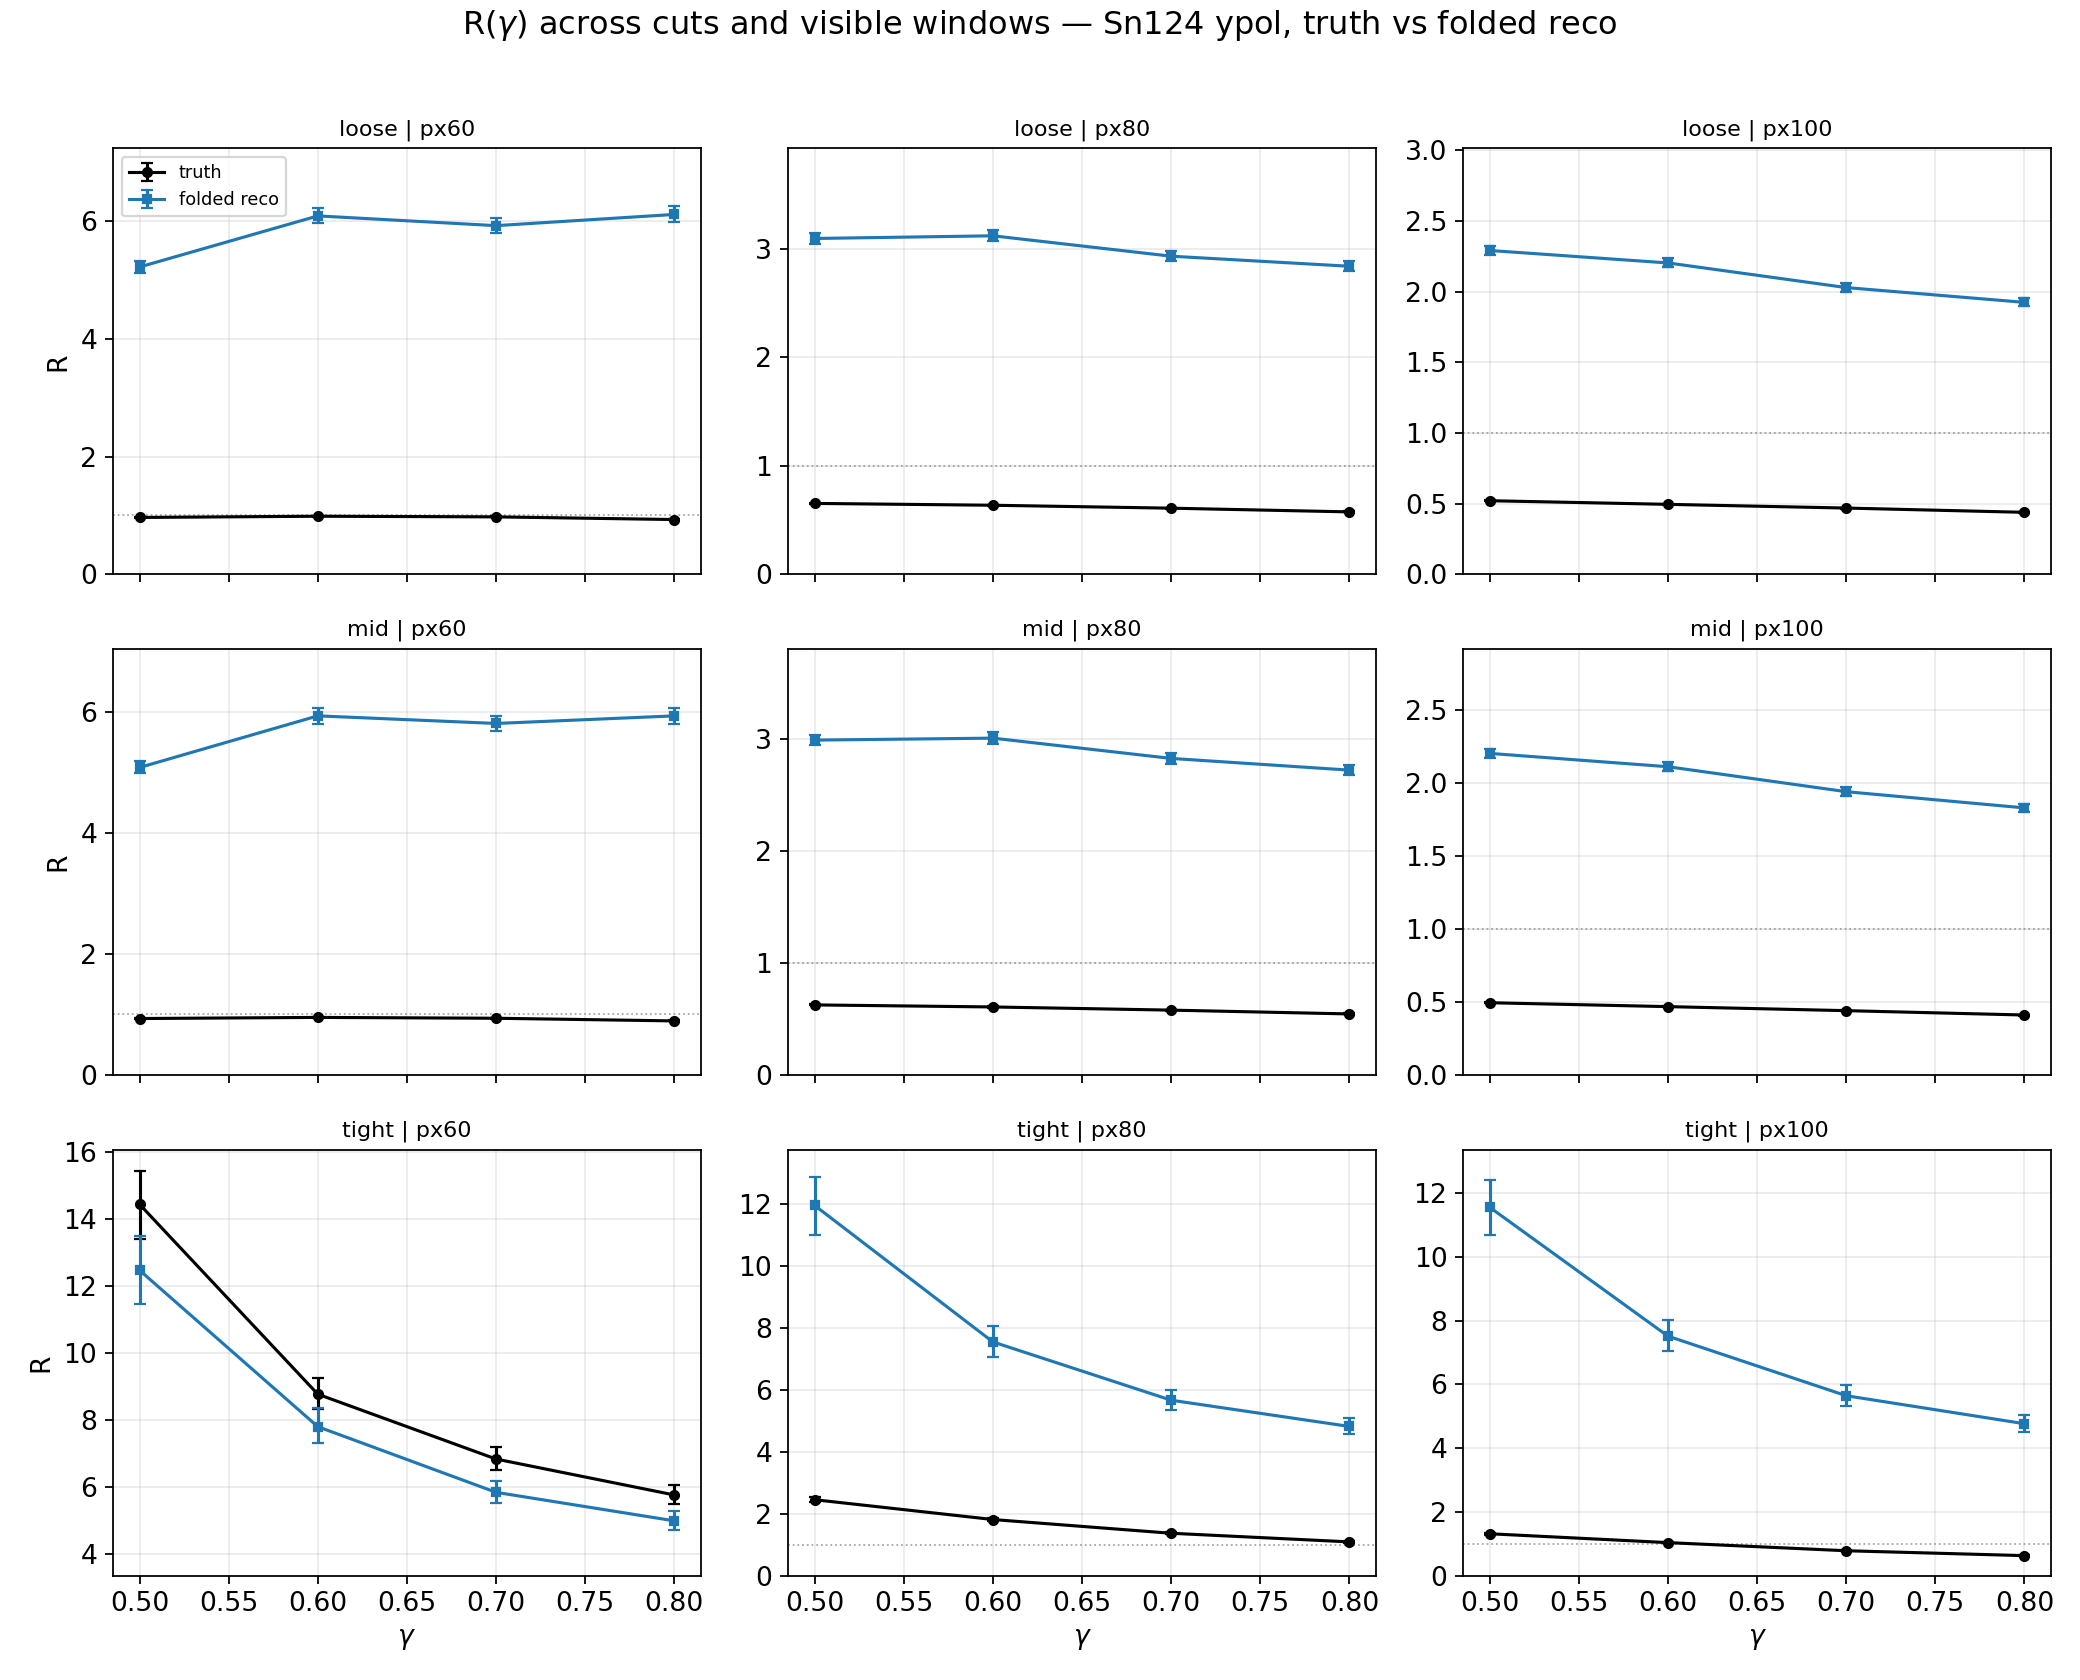
\includegraphics[width=\linewidth]{cut_diagnostics/r_vs_gamma_cut_grid_ypol.png}
  \caption{ypol $R(\gamma)$ 在 9 组 cut (行 = loose/mid/tight，列 = px60/px80/px100) 下的全貌，Sn124。黑点 = truth-level $R$，蓝点 = folded reco $R$，误差棒为 bootstrap。}
\end{figure}

\begin{figure}[H]
  \centering
  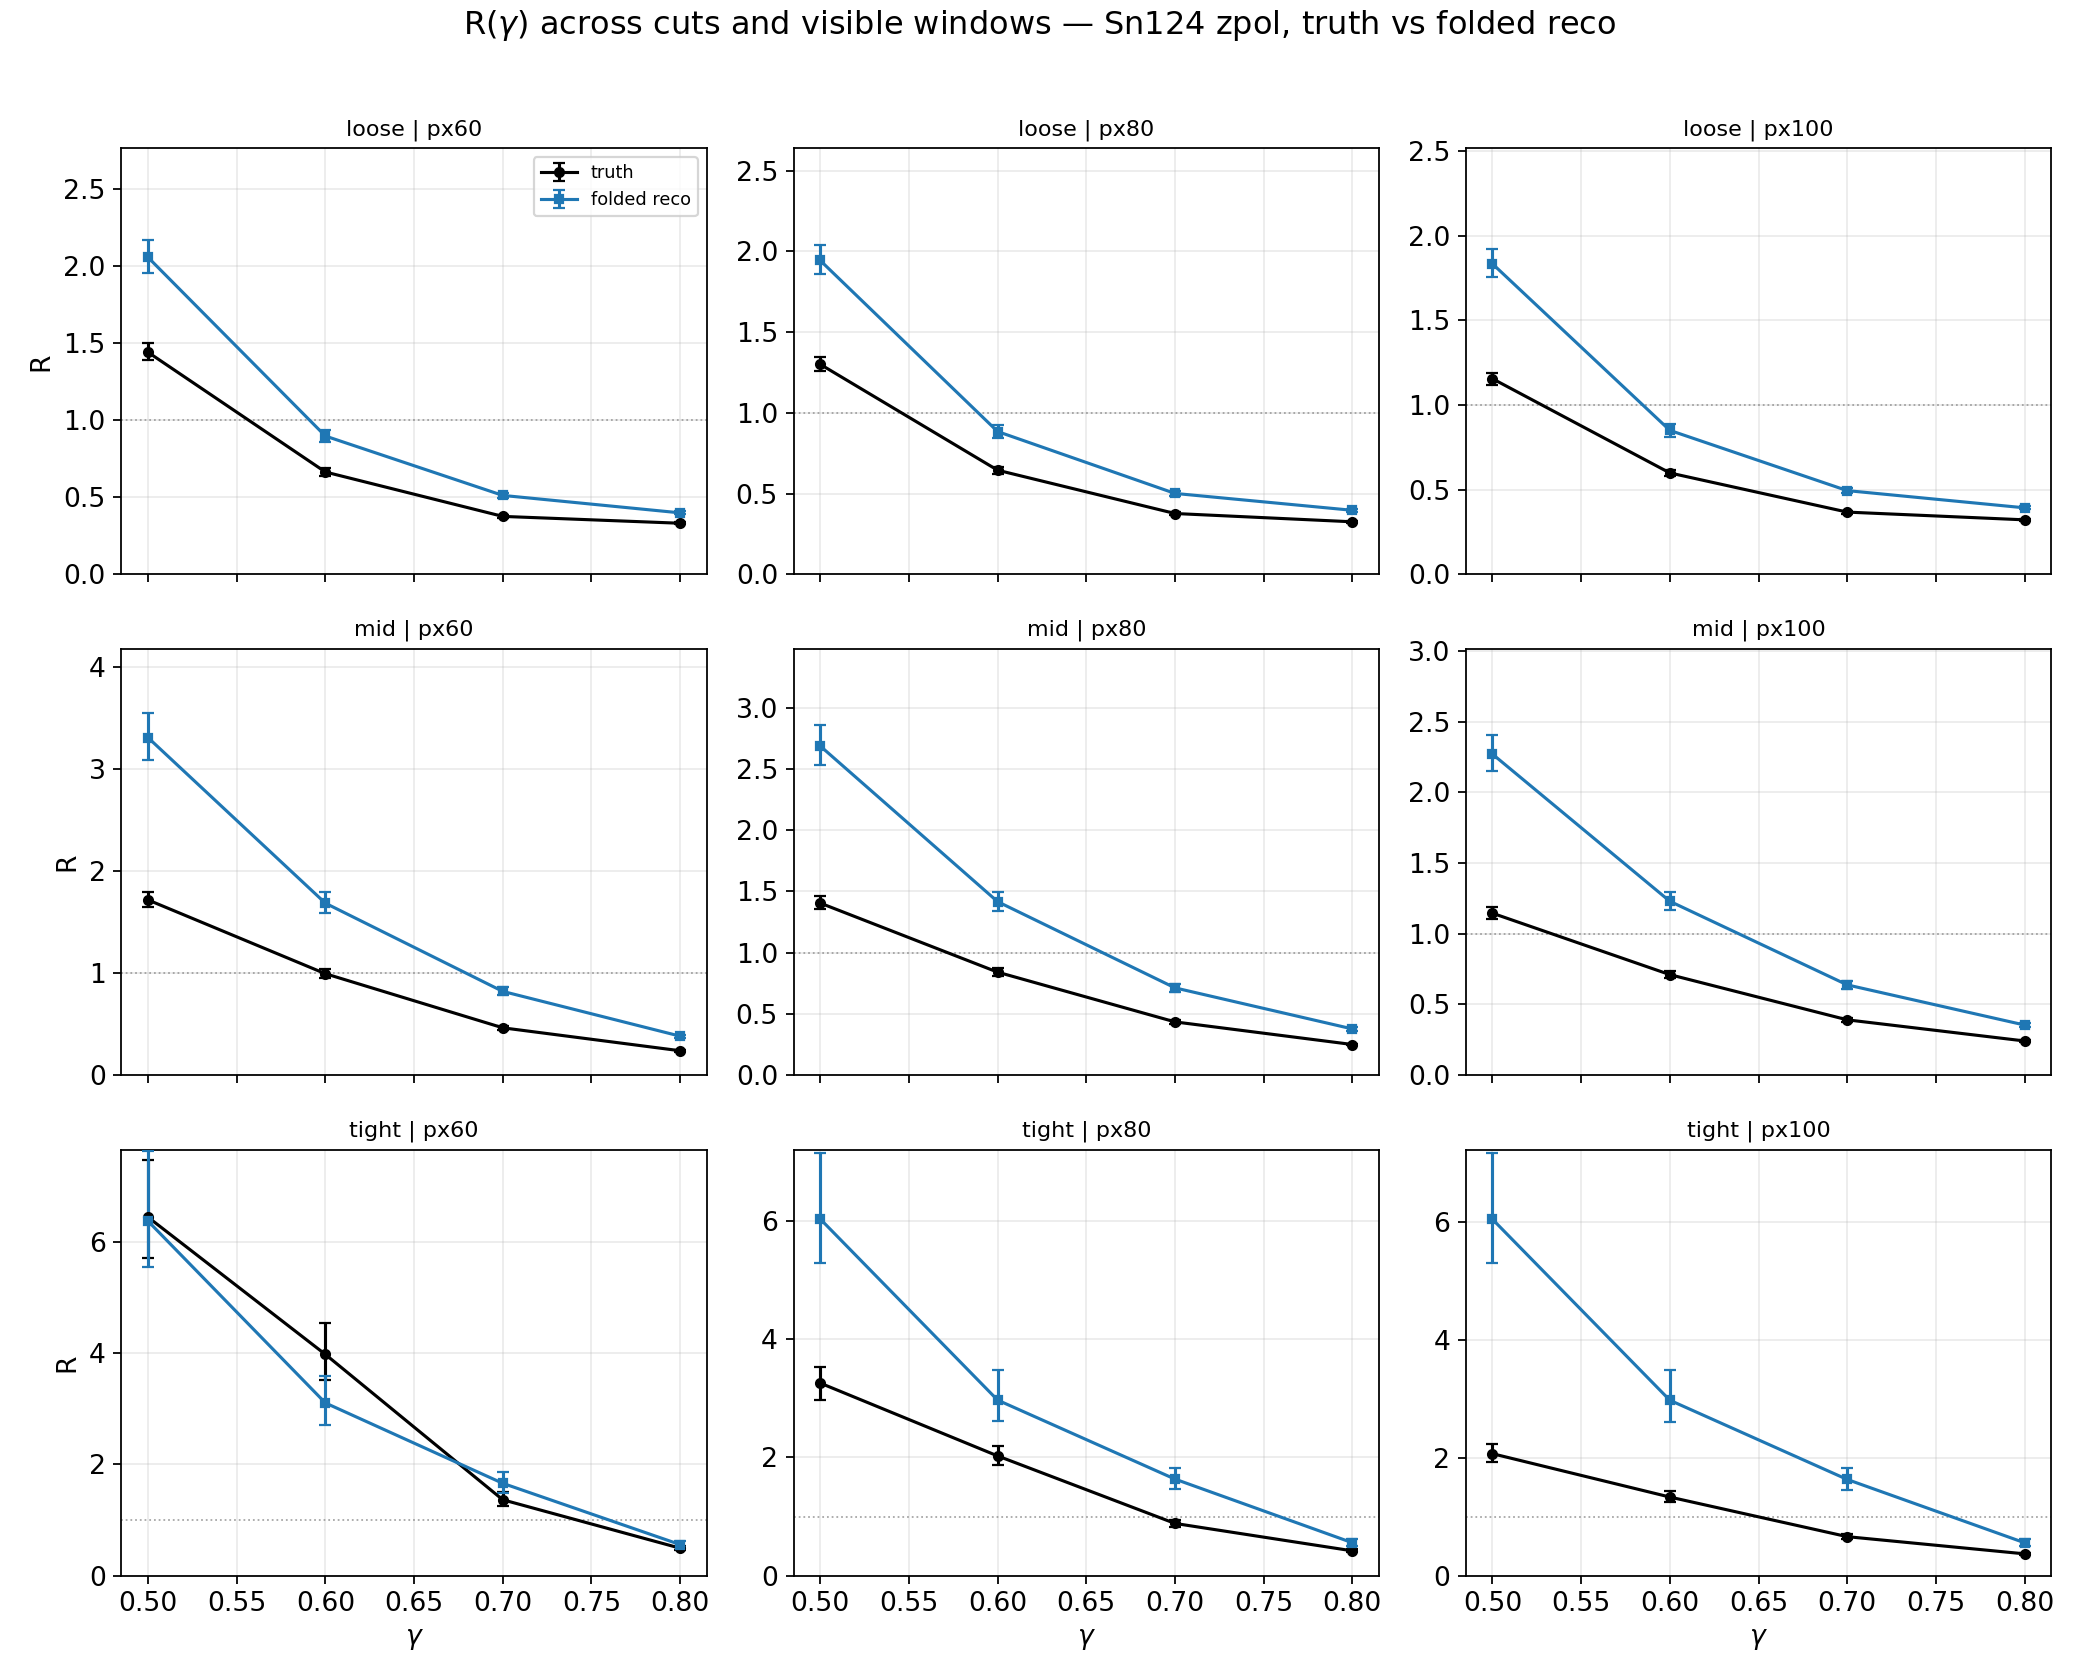
\includegraphics[width=\linewidth]{cut_diagnostics/r_vs_gamma_cut_grid_zpol.png}
  \caption{zpol 的对应 9 组 cut 网格。}
\end{figure}

要点: \texttt{loose}$\to$\texttt{tight} 使 ypol 的 $R$ 单调上升、zpol 的 $R$ 单调下降 (事件选择越来越偏向某一符号)；px60$\to$px100 使 $R$ 增大 (更大的 visible window 保留了更多 NEBULA 看不到的负 $p_{x,n}$ 分支)；reco 与 truth 的 gap 在 tight px60 最小。$\gamma$ 敏感性 (曲线斜率) 在全部 9 组里都保留，但 tight px60 的 truth/reco 一致性最好。

\subsection{$\Delta p_x$ 形状: truth vs reco}

\begin{figure}[H]
  \centering
  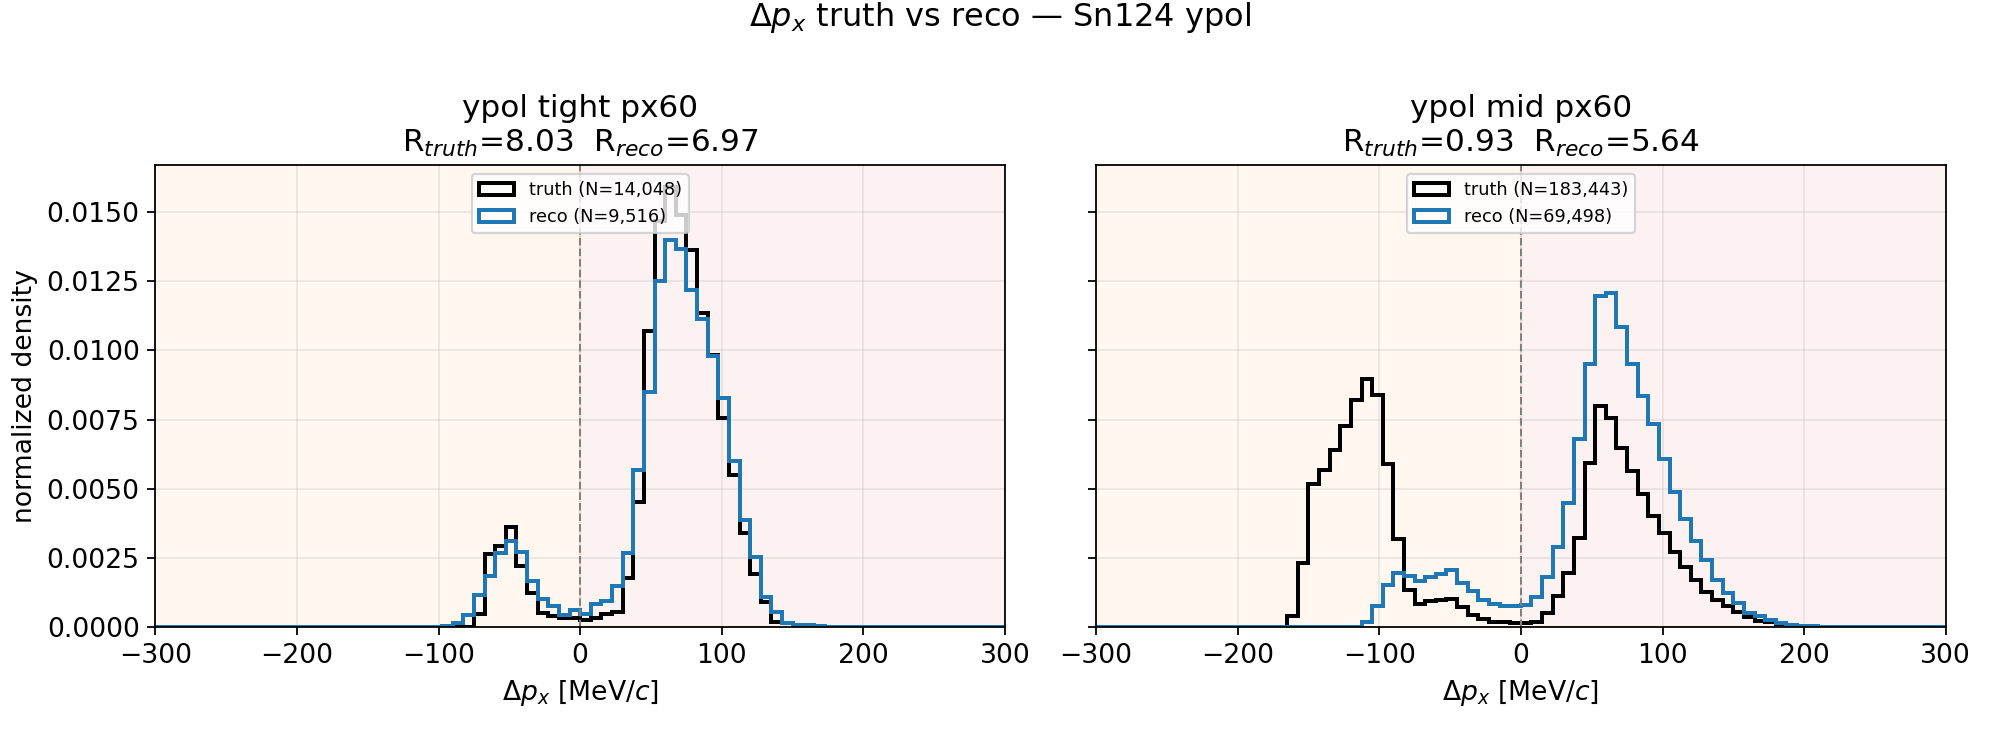
\includegraphics[width=\linewidth]{cut_diagnostics/dpx_truth_vs_reco_overlay_ypol.png}
  \caption{ypol 归一化 $\Delta p_x$ 直方图。黑 = truth (truth 事件面 + truth 动量)，蓝 = reco (reco 事件面 + NN 质子 + reconstructed 中子)。红色背景 = $\Delta p_x>0$ ($R$ 分子)，橙色 = $\Delta p_x<0$ ($R$ 分母)。tight px60 与 mid px60 并排。}
\end{figure}

\begin{figure}[H]
  \centering
  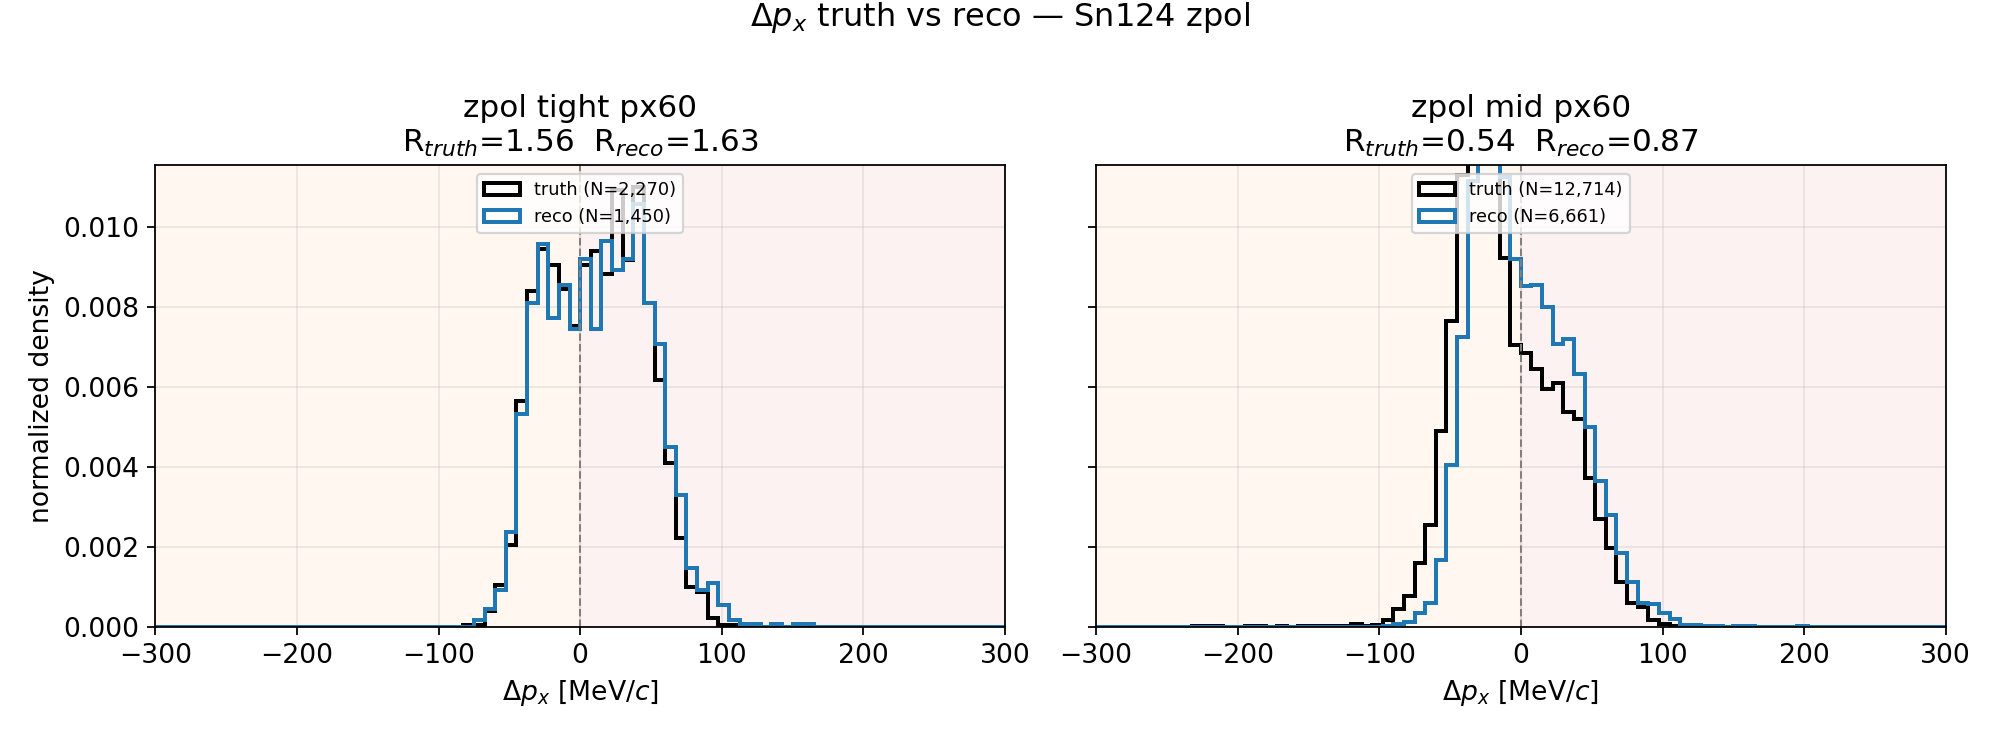
\includegraphics[width=\linewidth]{cut_diagnostics/dpx_truth_vs_reco_overlay_zpol.png}
  \caption{zpol 的对应 $\Delta p_x$ truth vs reco 叠加。}
\end{figure}

reco 分布的峰位和宽度与 truth 接近，符号迁移主要发生在尾部；ypol 的不对称性 (正侧远大于负侧) 在 truth 和 reco 里都清楚可见。图标题里同时给出对应的 $R_{\mathrm{truth}}$ 和 $R_{\mathrm{reco}}$。

\subsection{相空间覆盖 (truth level)}

\begin{figure}[H]
  \centering
  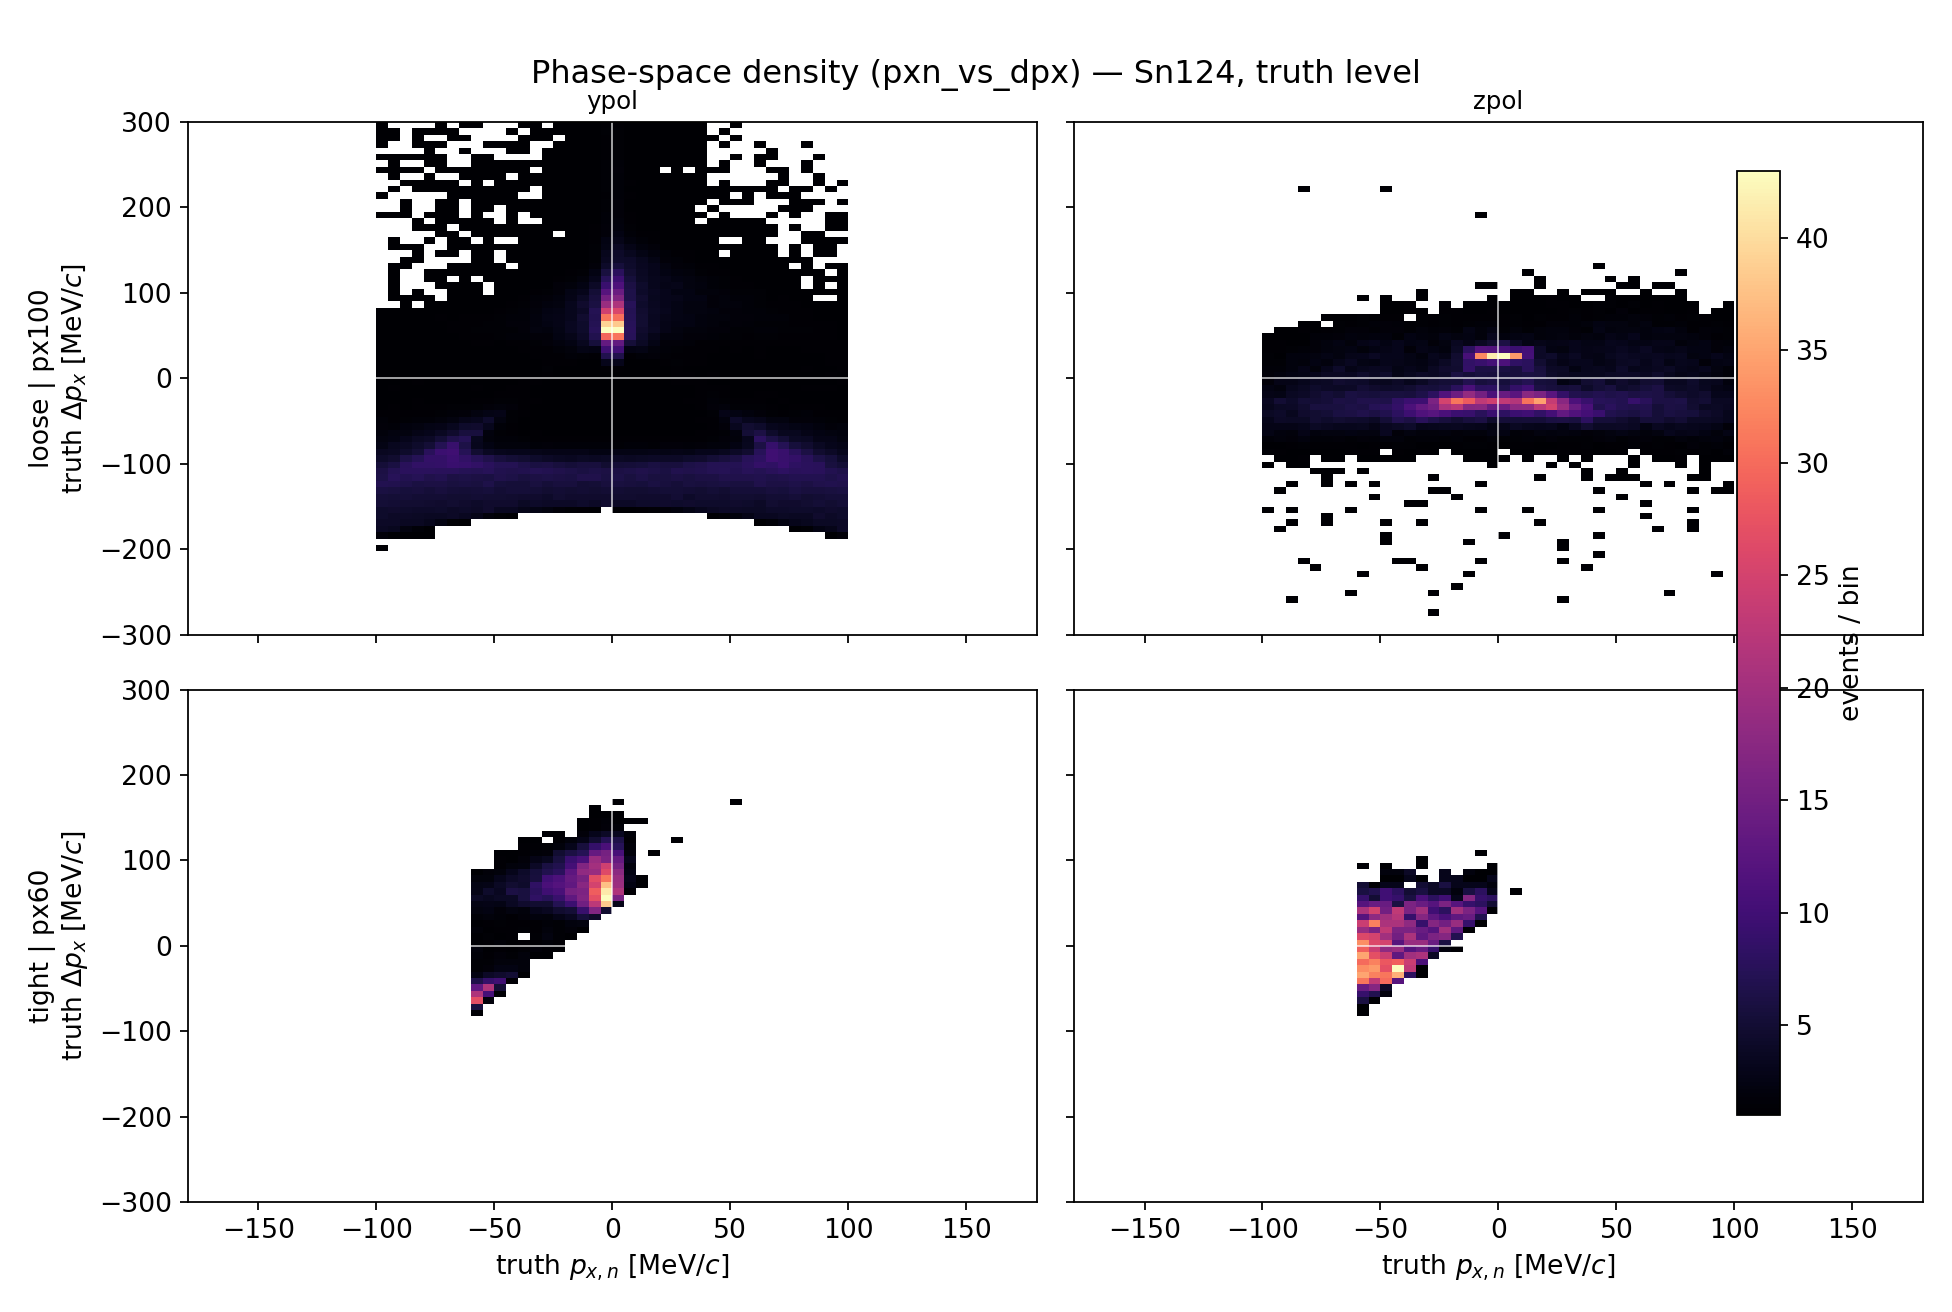
\includegraphics[width=0.96\linewidth]{cut_diagnostics/phase_density_pxn_vs_dpx.png}
  \caption{\textbf{Truth-level} 相空间密度 (事件计数/格，不是效率)。上排 = loose px100，下排 = tight px60，列 = ypol/zpol。它回答的是 ``这套 cut 在 truth 相空间里选了哪一块区域''。}
\end{figure}

\begin{figure}[H]
  \centering
  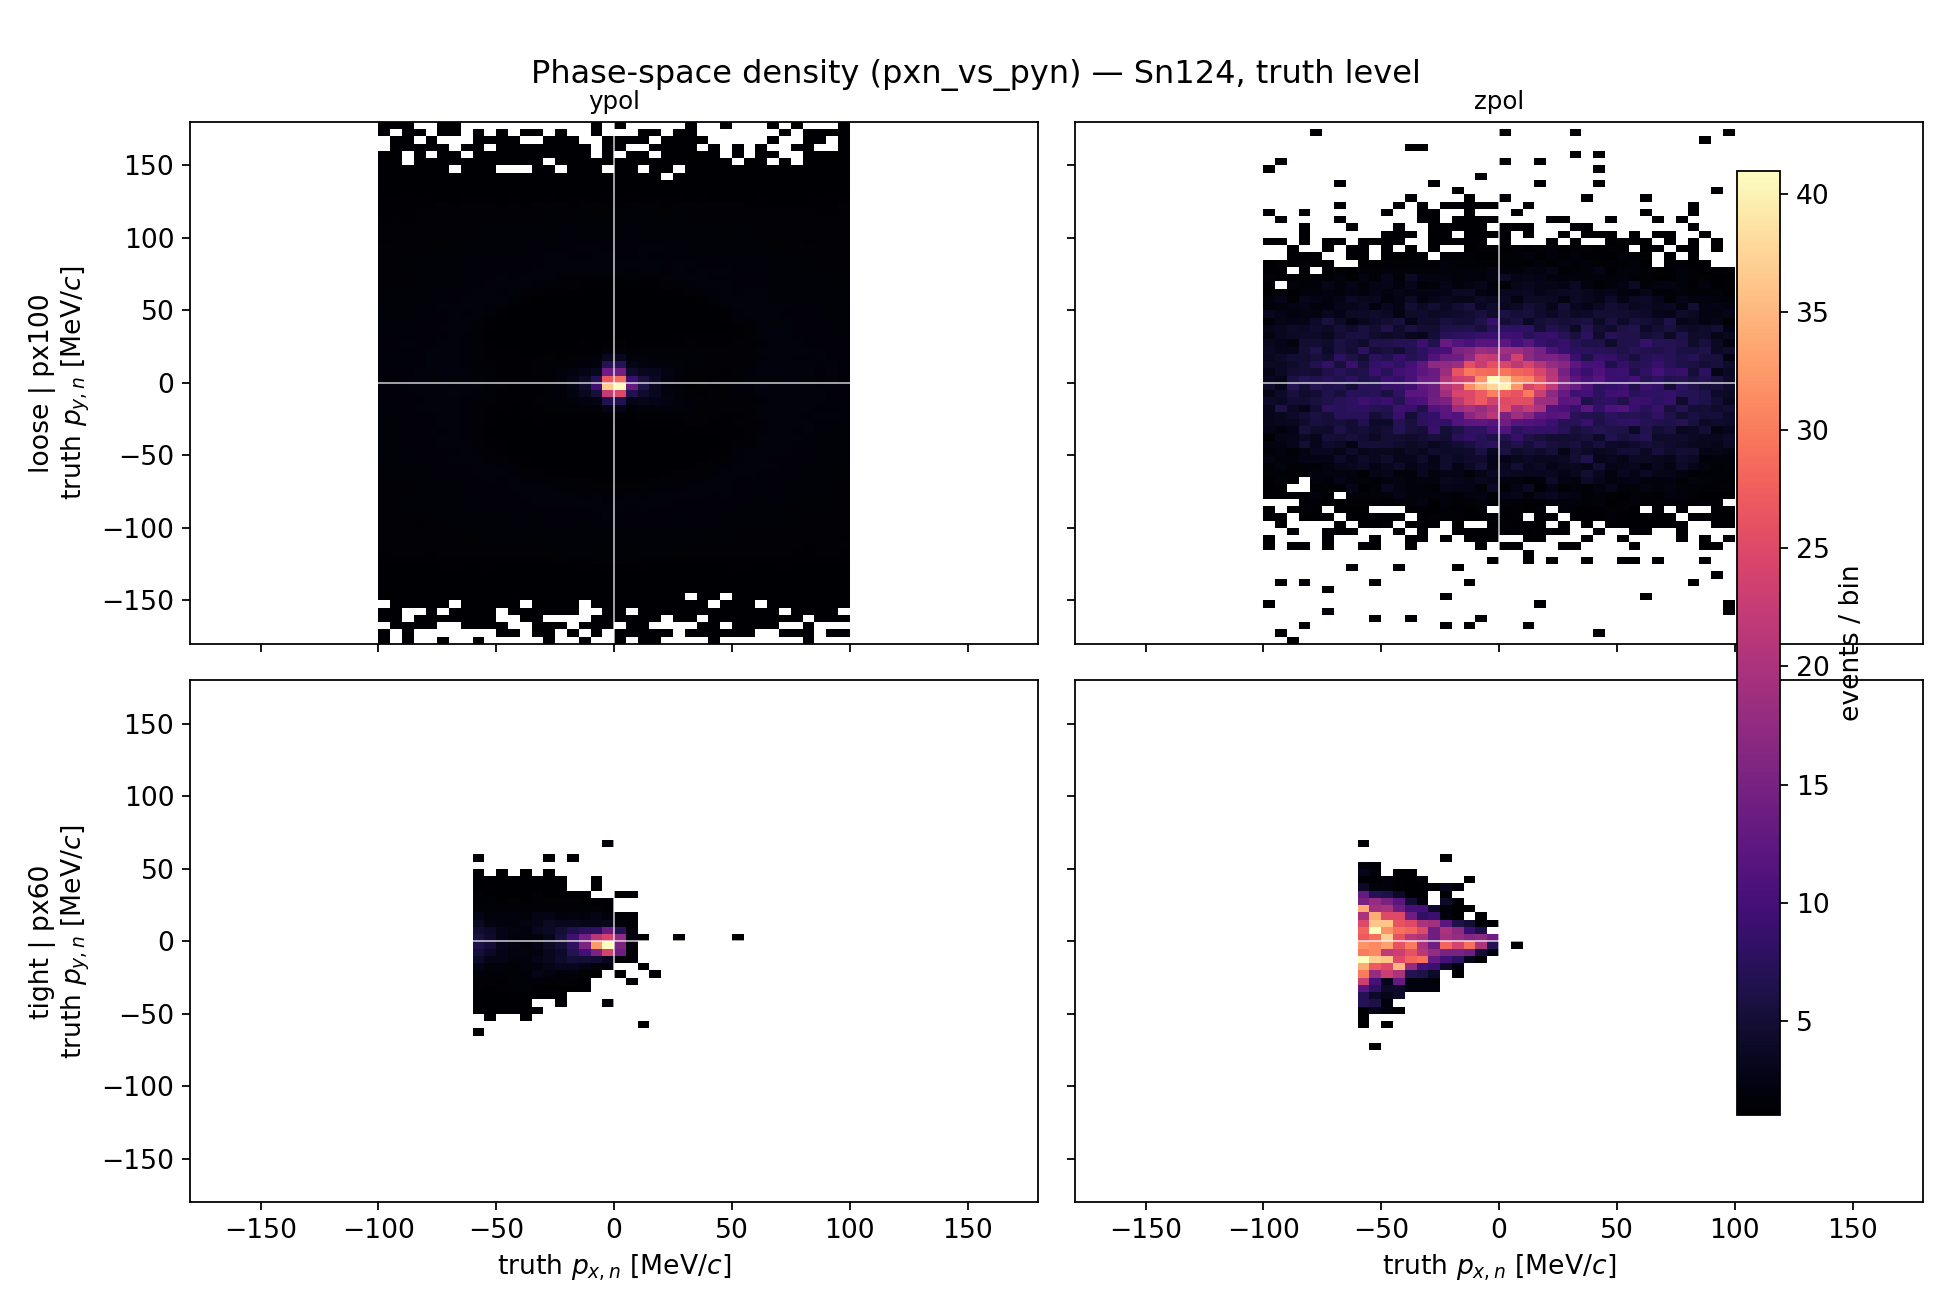
\includegraphics[width=0.96\linewidth]{cut_diagnostics/phase_density_pxn_vs_pyn.png}
  \caption{同上，truth $p_{x,n}$ vs $p_{y,n}$ 中子横向平面。}
\end{figure}

\begin{figure}[H]
  \centering
  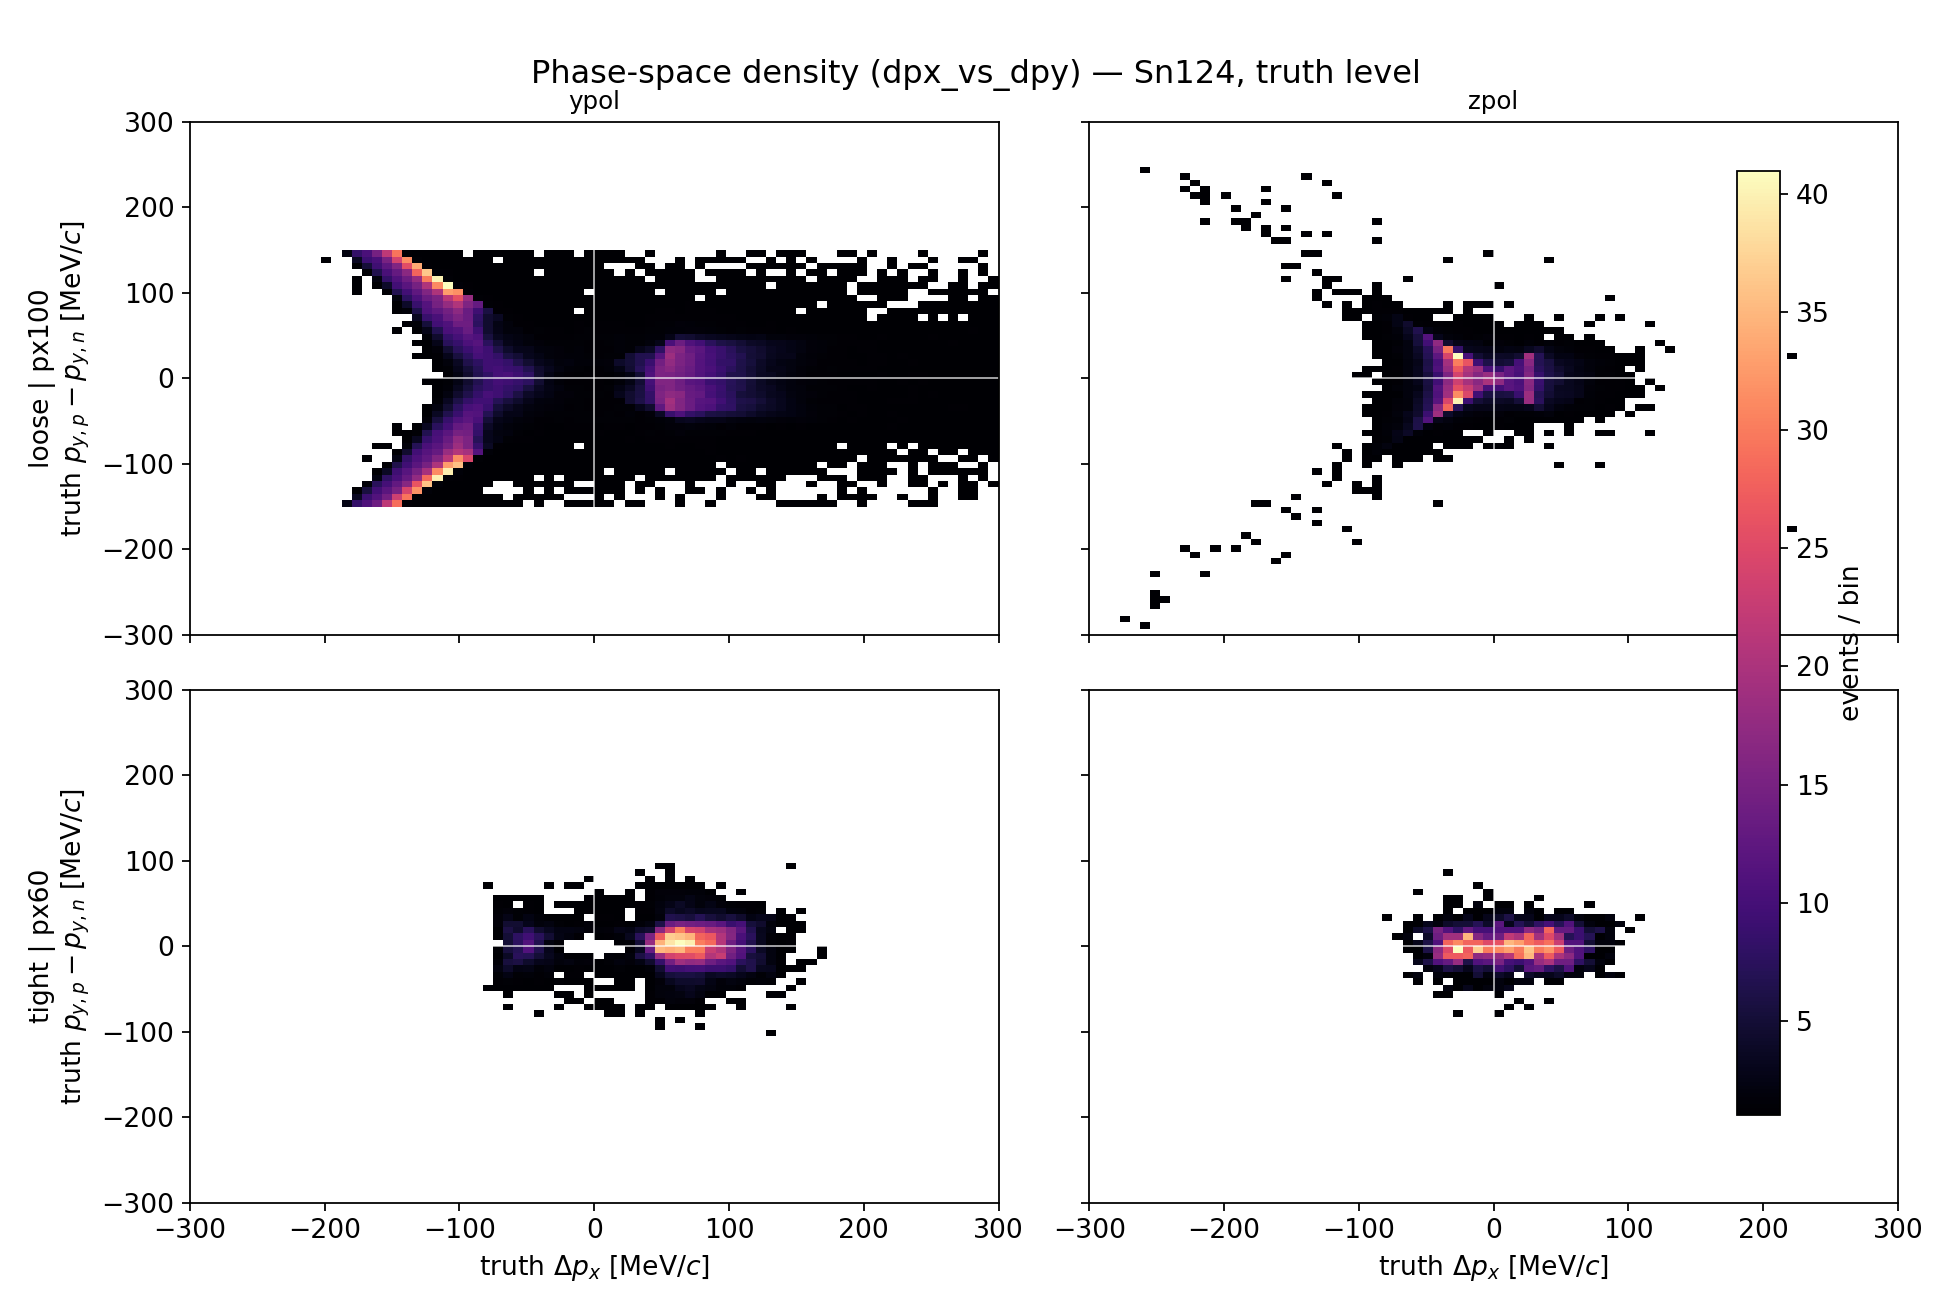
\includegraphics[width=0.96\linewidth]{cut_diagnostics/phase_density_dpx_vs_dpy.png}
  \caption{同上，truth $\Delta p_x$ vs $(p_{y,p}-p_{y,n})$ 动量不对称平面。tight 把事件压到反应面附近。}
\end{figure}

这三张是 \textbf{truth-level} 相空间密度 (事件计数，非效率)。tight px60 把中子 $|p_{x,n}|<60$ 的窄条切出来，$\Delta p_x$ 集中在正值侧 (ypol)；loose px100 的覆盖范围大得多。reco-level 的 truth$\to$reco 迁移是另一个问题，由“Detector folding 技术诊断”中的 response matrix 覆盖——本节看的是 cut 的几何选择，不是探测器 smearing。

\subsection{不同 cut 下的 neutron efficiency}

\begin{figure}[H]
  \centering
  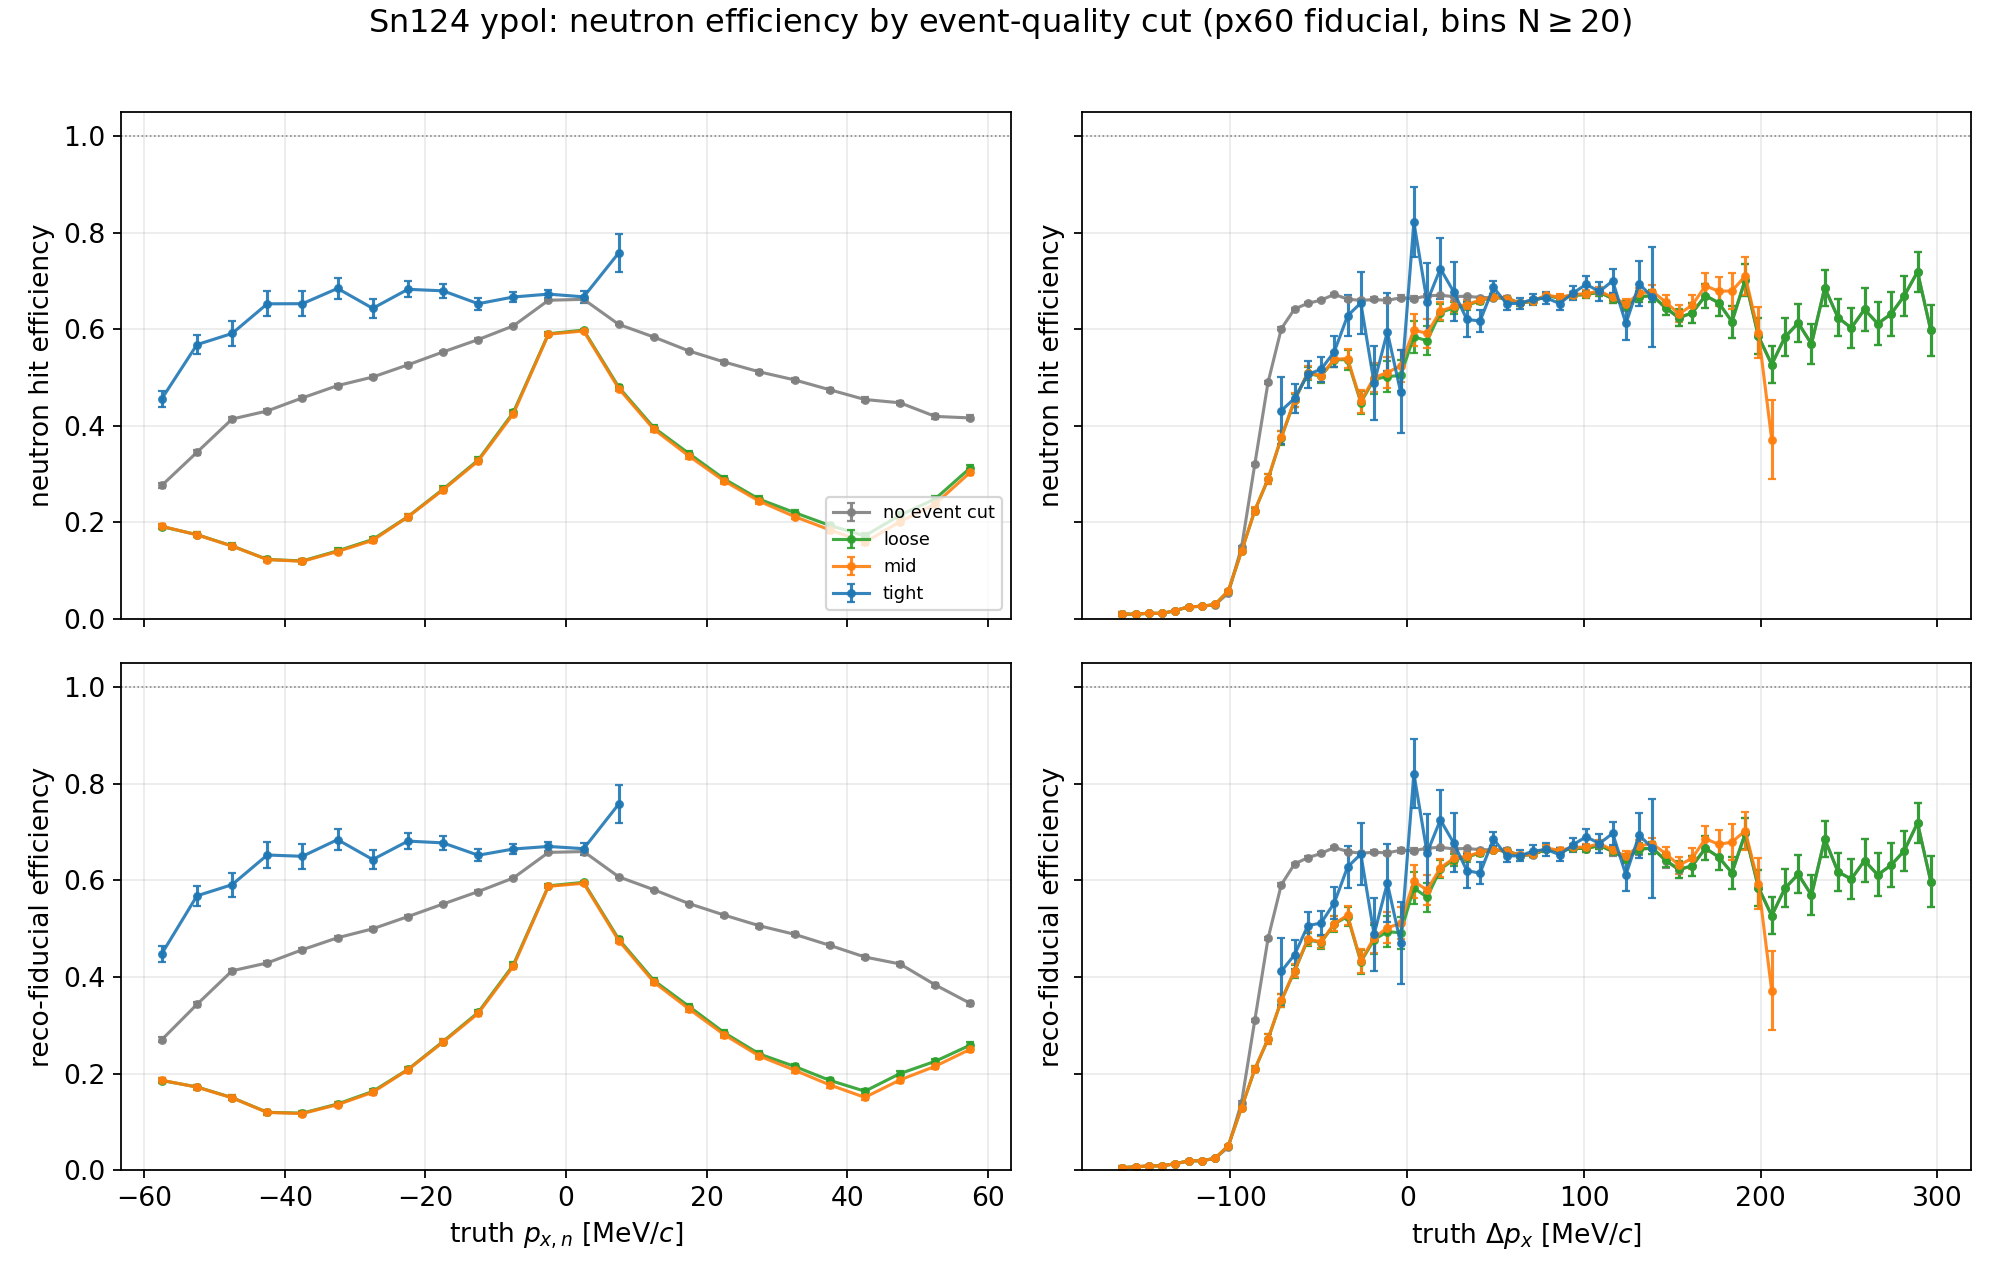
\includegraphics[width=\linewidth]{cut_diagnostics/neutron_efficiency_1d_by_cut_ypol.png}
  \caption{ypol neutron efficiency 随 event-quality cut 的变化 (px60 truth fiducial)。四条曲线 = none (无事件选择) / loose / mid / tight。上排 = neutron hit efficiency，下排 = reco-fiducial efficiency；左列 vs truth $p_{x,n}$，右列 vs truth $\Delta p_x$。效率定义为 $\epsilon(x)=N_{\mathrm{hit}}(x\text{-bin})/N_{\mathrm{fid}}(x\text{-bin})$，只画 $N_{\mathrm{fid}}\geq20$ 的 bin。}
\end{figure}

\begin{figure}[H]
  \centering
  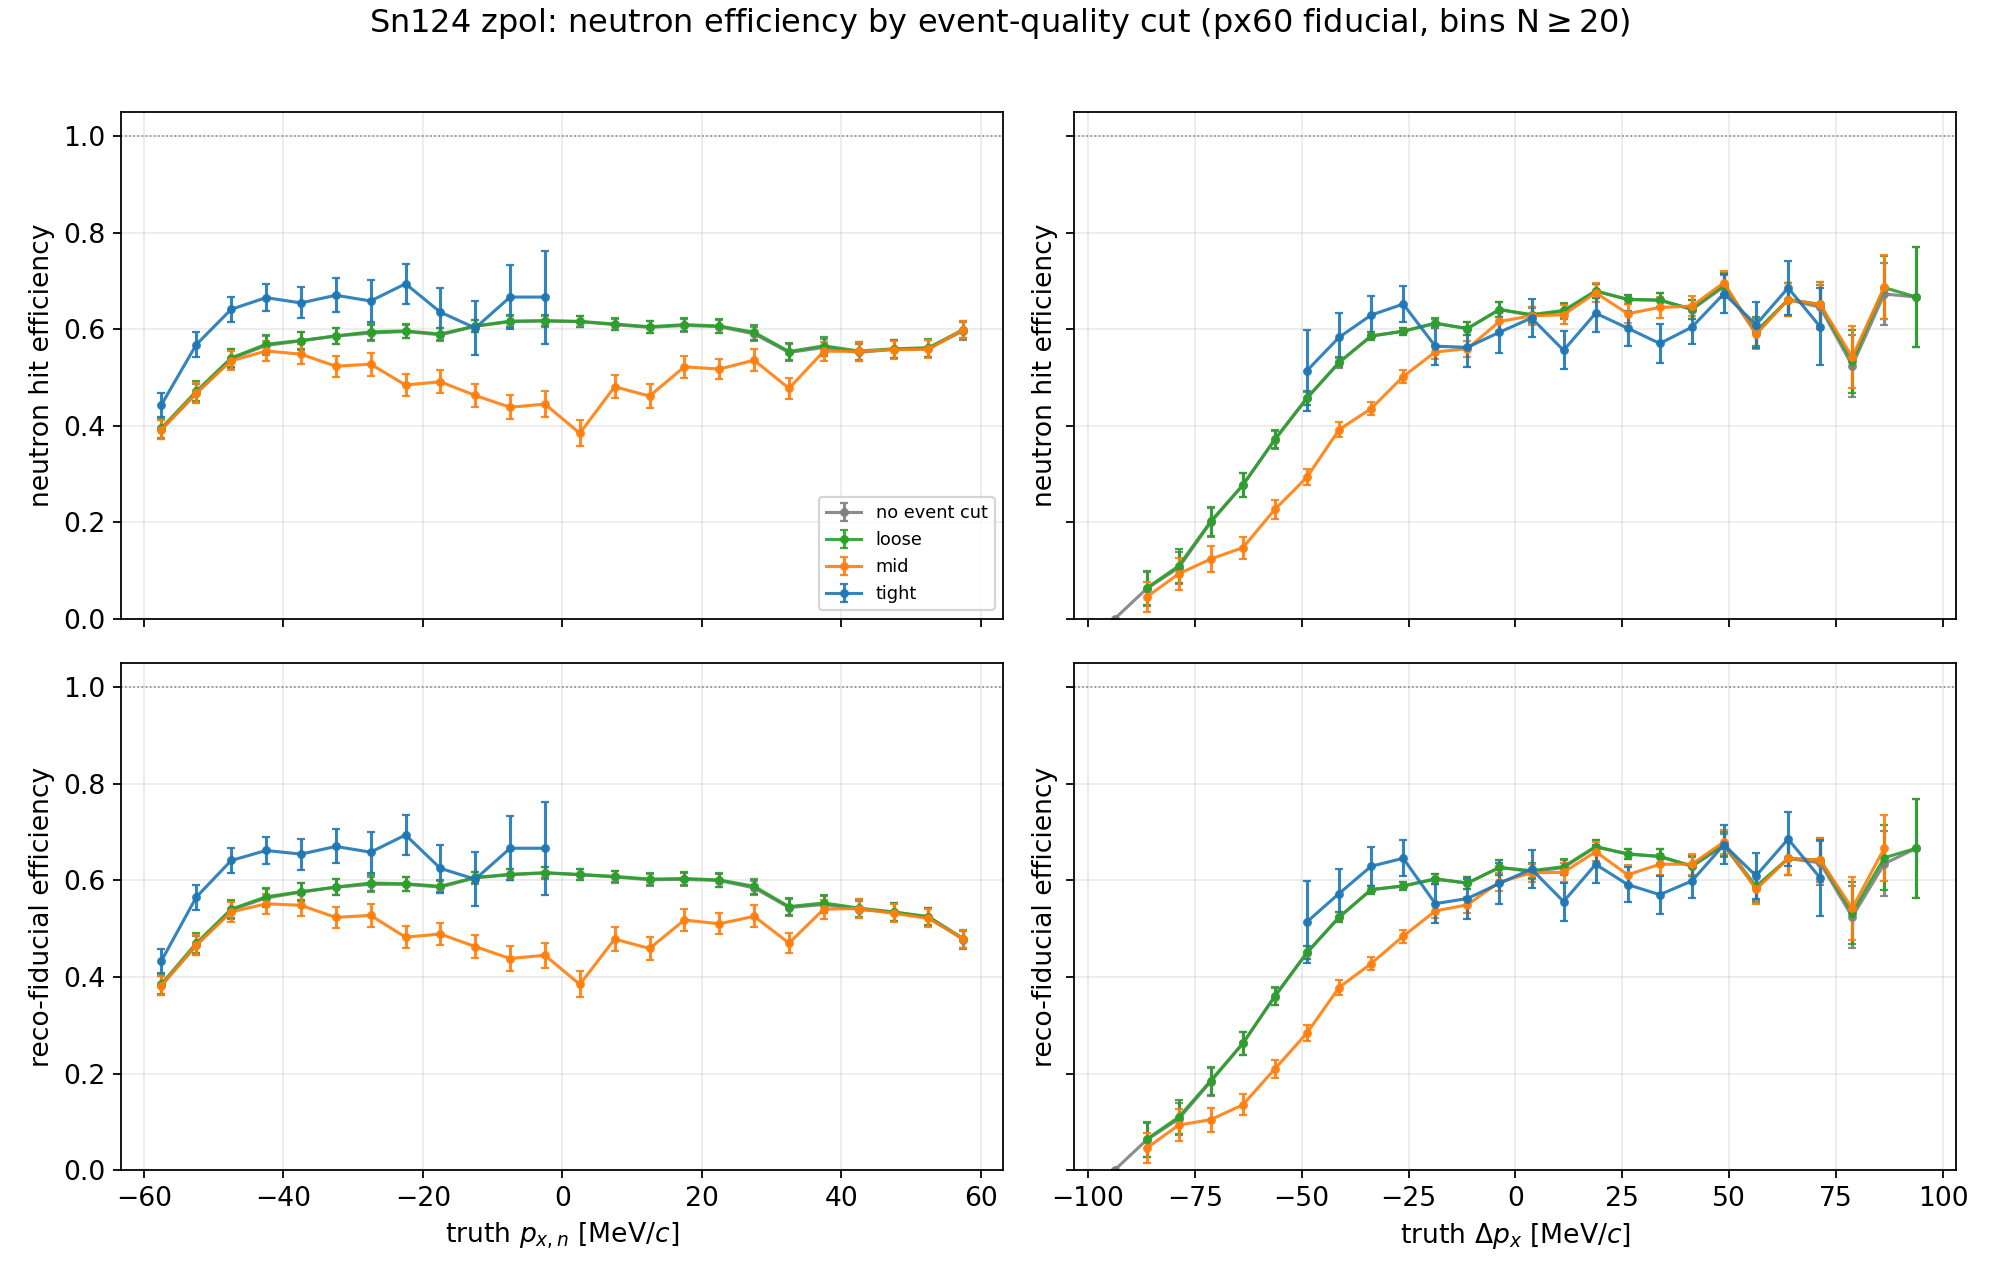
\includegraphics[width=\linewidth]{cut_diagnostics/neutron_efficiency_1d_by_cut_zpol.png}
  \caption{zpol 的对应效率曲线。zpol 的 ``none'' 曲线统计有限，部分 bin 误差较大。}
\end{figure}

\begin{figure}[H]
  \centering
  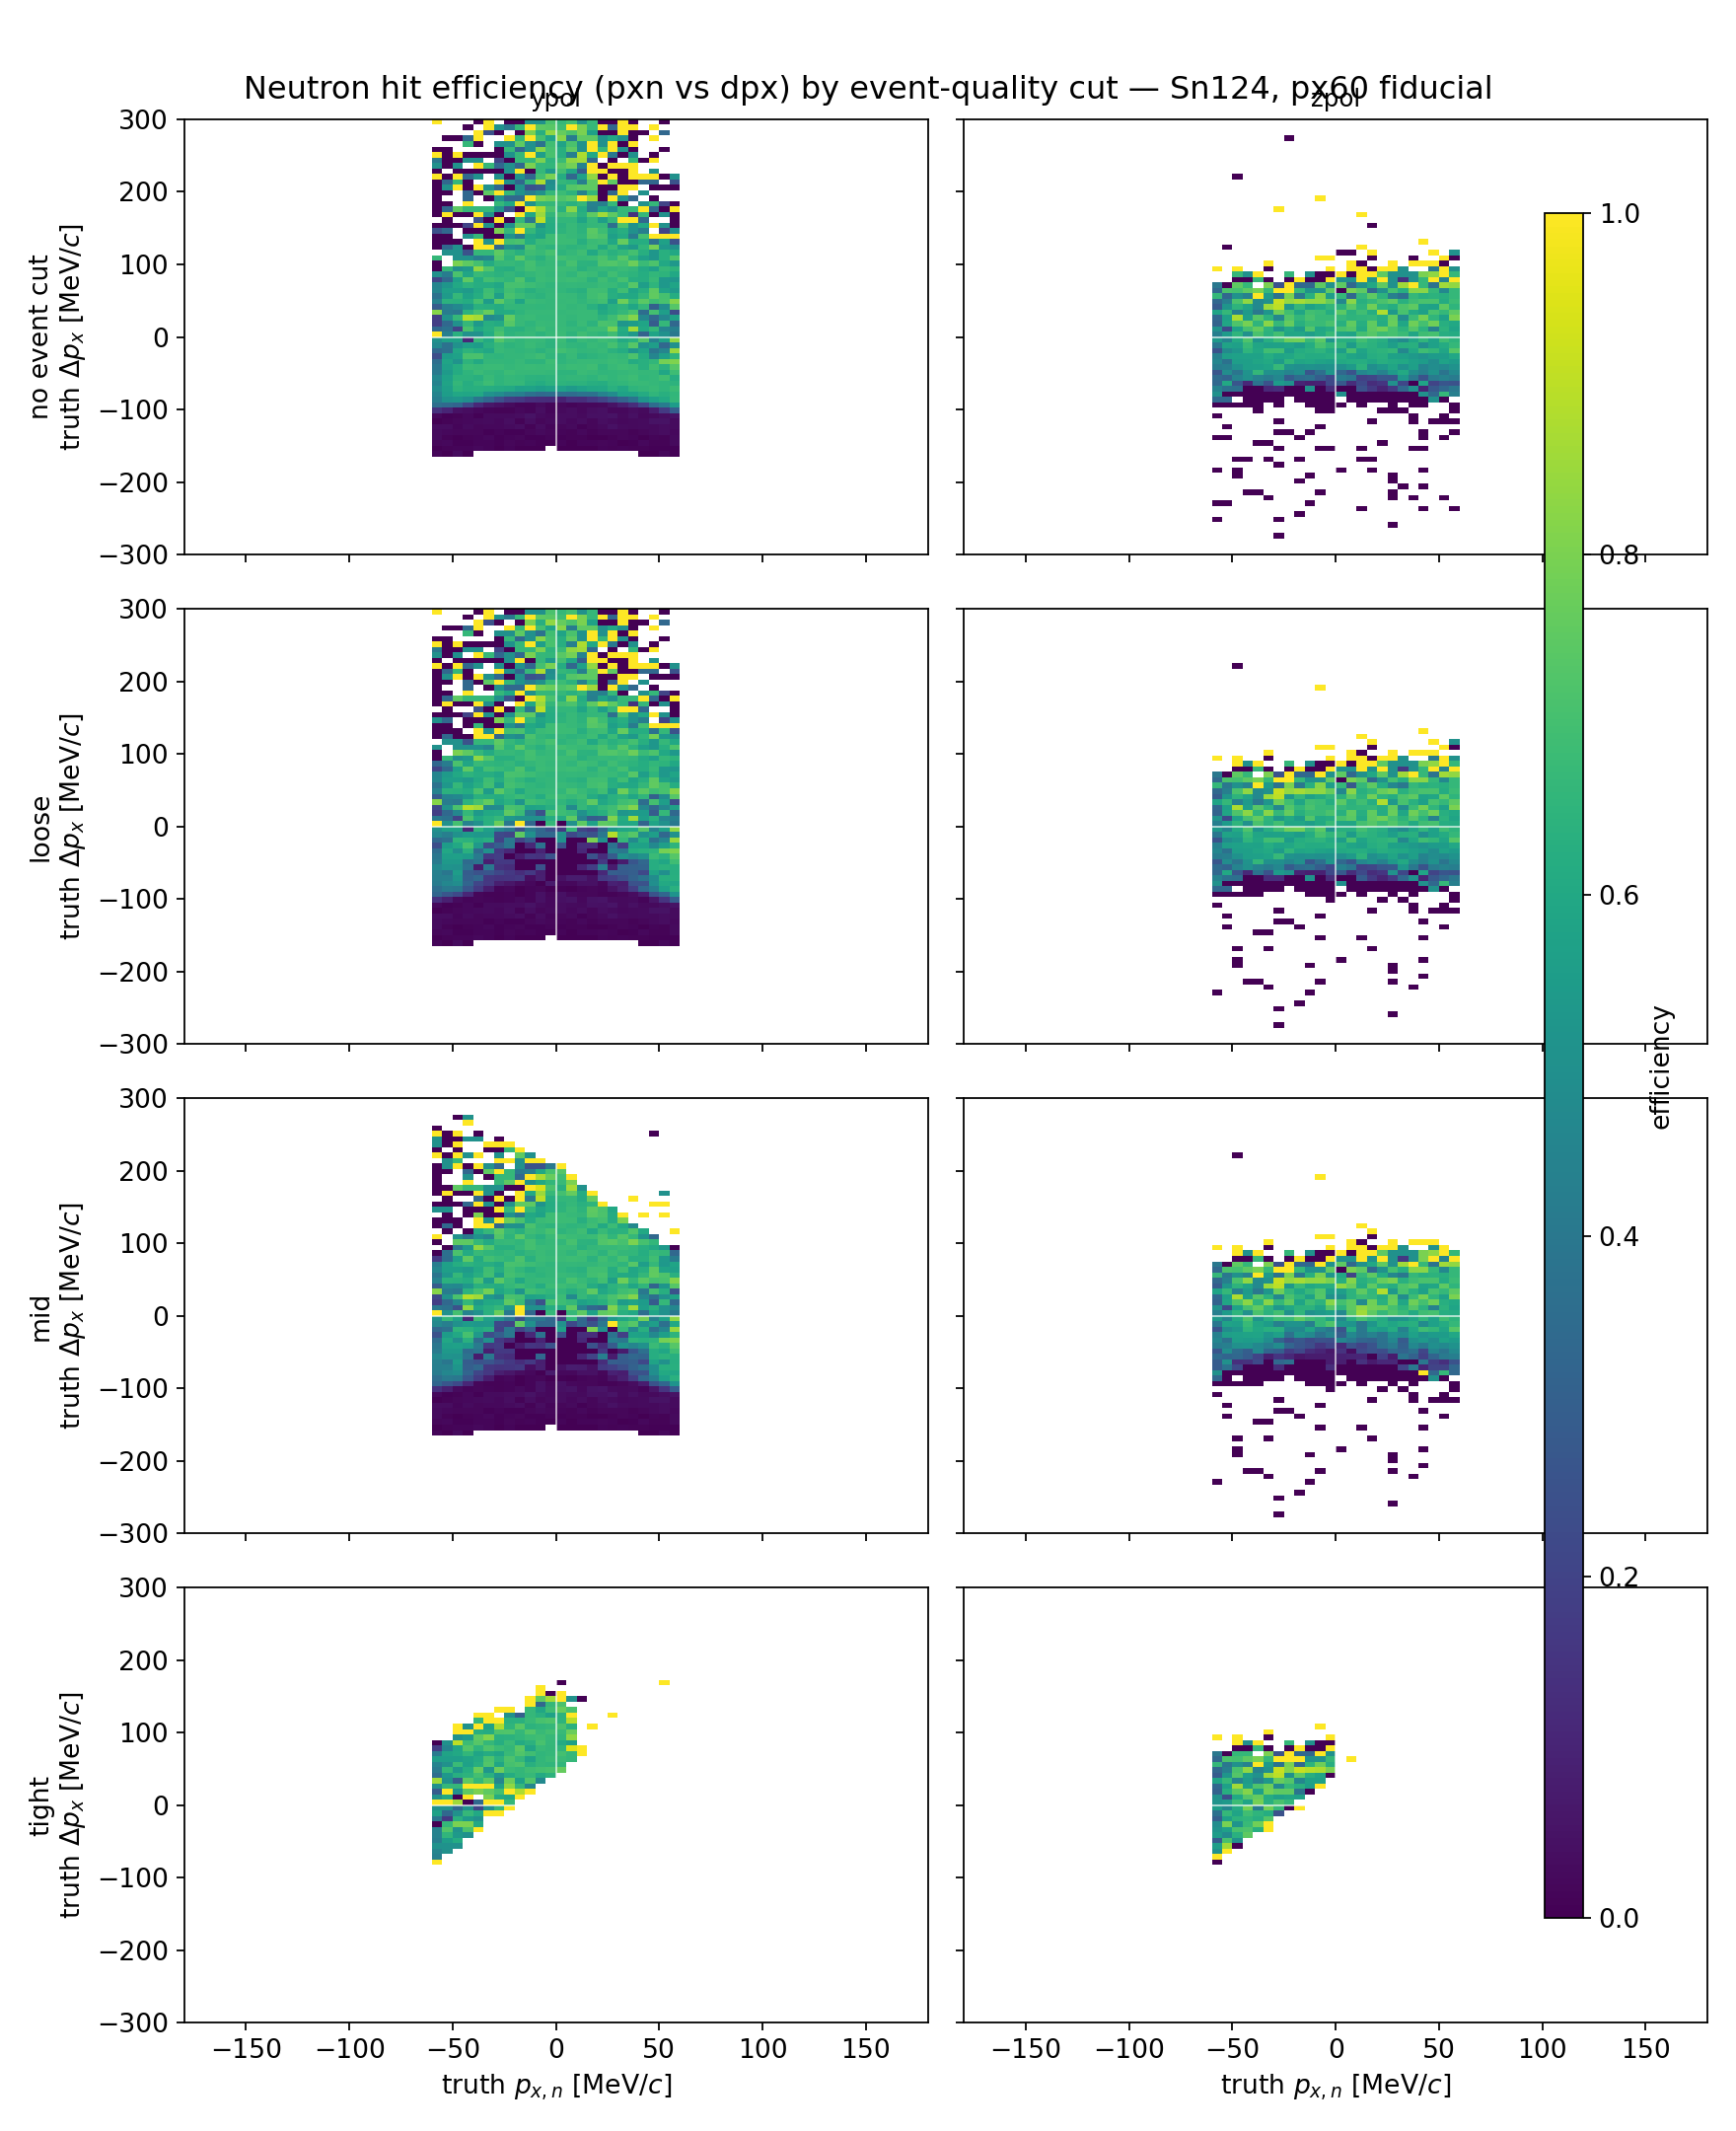
\includegraphics[width=0.85\linewidth]{cut_diagnostics/neutron_efficiency_2d_pxn_vs_dpx_by_cut.png}
  \caption{Neutron hit efficiency 的二维 ($p_{x,n}$, $\Delta p_x$) 热图，按 event-quality cut 分行 (none/loose/mid/tight)，列为 ypol/zpol。全部使用 px60 truth fiducial。}
\end{figure}

要点: 从 none 到 tight，效率曲线的形状基本一致 (核心区 $\epsilon\sim$0.55--0.70)，说明 event-quality cut 主要改变的是进入样本的相空间区域 (哪些 $p_{x,n}$/$\Delta p_x$ 的 bin 有足够统计)，而不是单 bin 内的探测效率本身。效率对 $p_{x,n}$ 符号的依赖 (ypol 中负 $p_{x,n}$ 侧效率偏低) 在 none 和 tight 下都存在——这是 NEBULA 几何的固有特征，cut 无法消除，只能通过缩小 visible window (px60) 把最严重的 sign-dependent 区域排除。

\subsection{无 px fiducial 的 neutron efficiency (全范围)}

\begin{figure}[H]
  \centering
  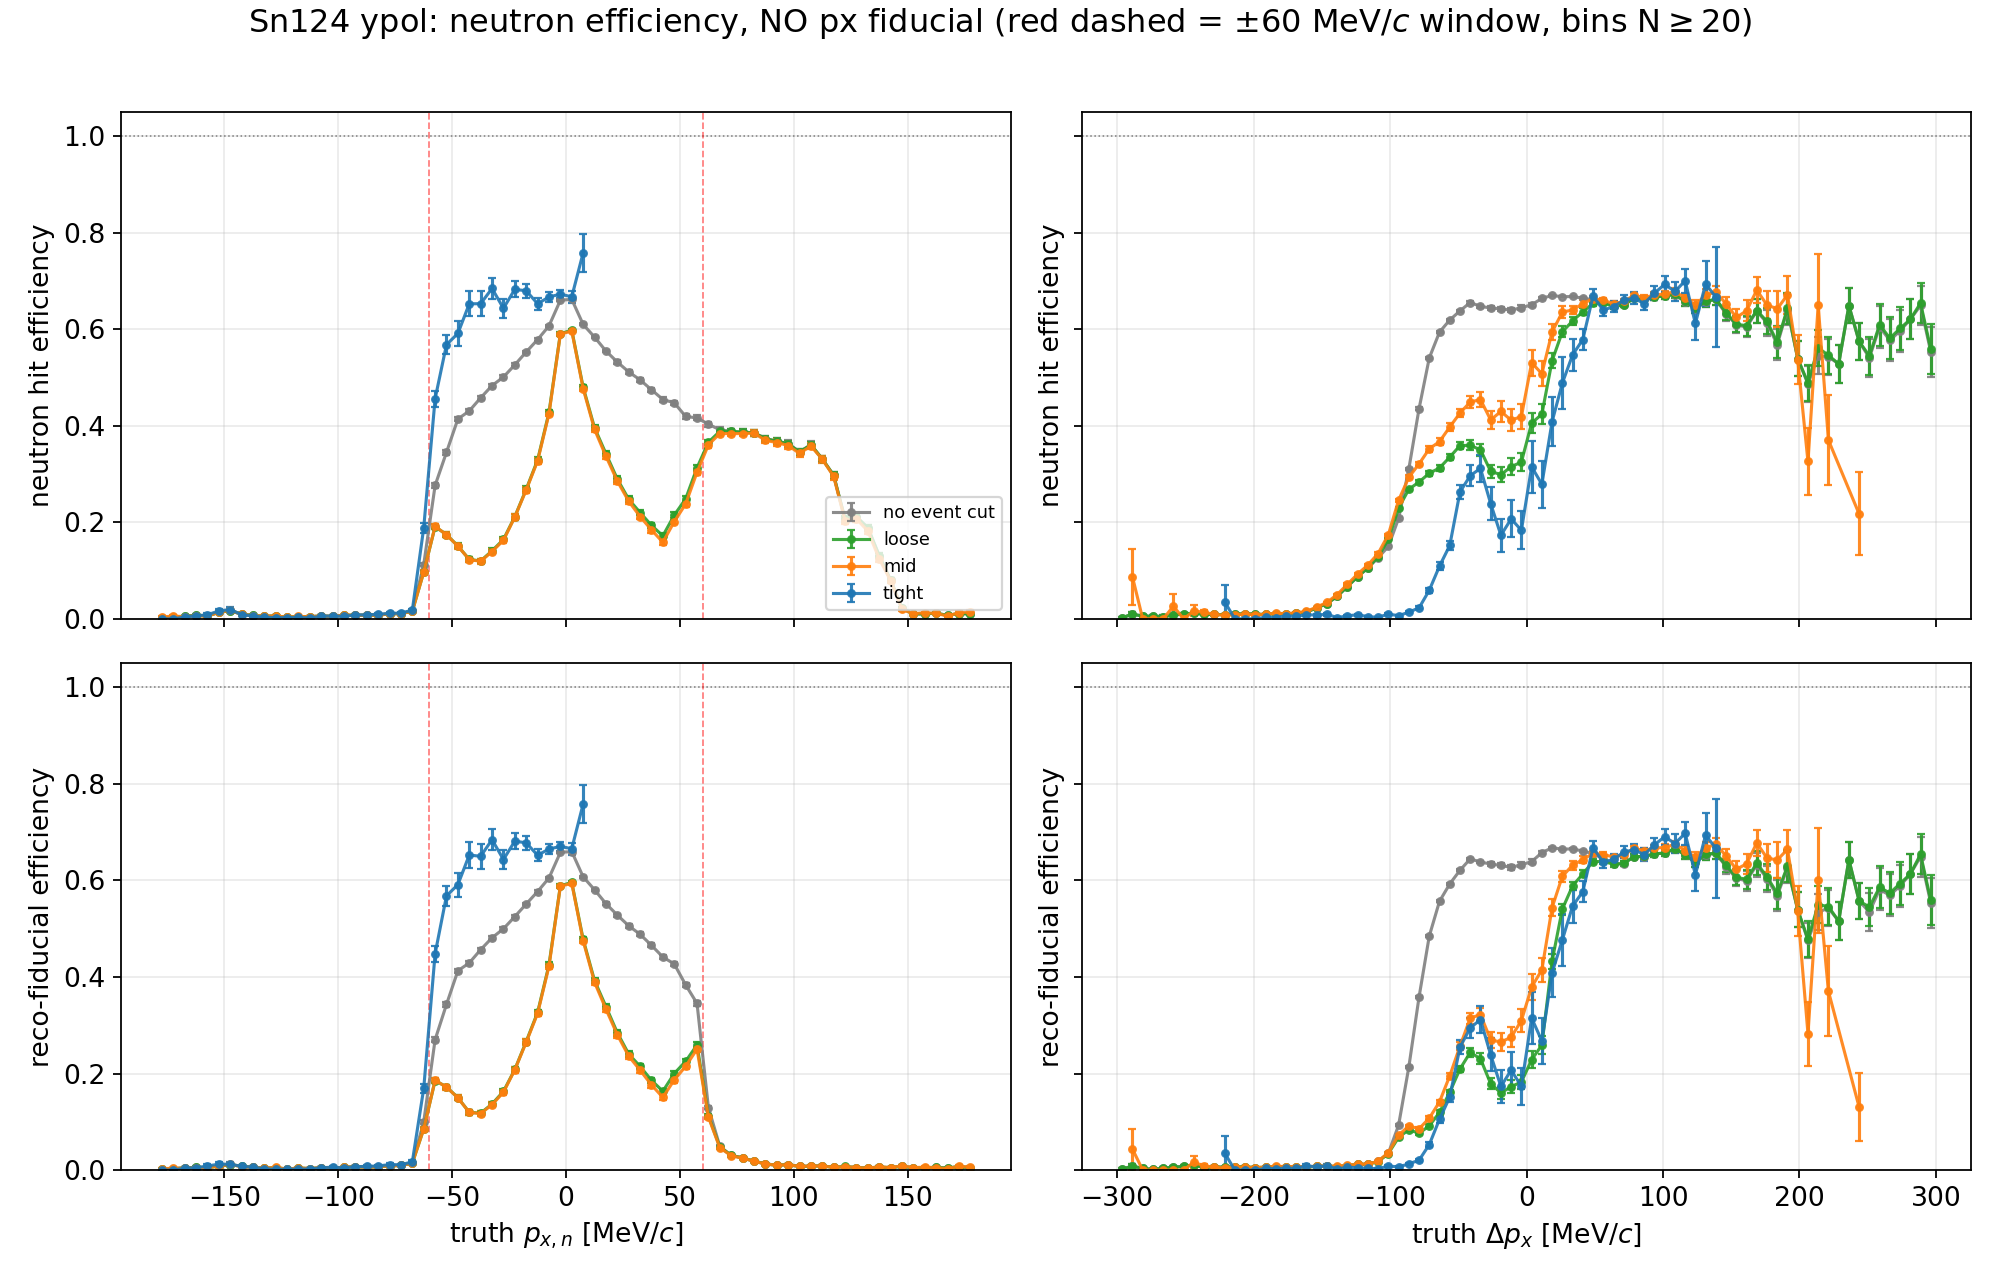
\includegraphics[width=\linewidth]{cut_diagnostics/neutron_efficiency_1d_nofiducial_ypol.png}
  \caption{ypol neutron efficiency 在 \textbf{无 px fiducial} 下的全范围曲线。红色虚线 = $\pm$60 MeV/$c$ (px60 窗口边界)。上排 = neutron hit efficiency，下排 = reco-fiducial efficiency。四条曲线同前 (none/loose/mid/tight)。}
\end{figure}

\begin{figure}[H]
  \centering
  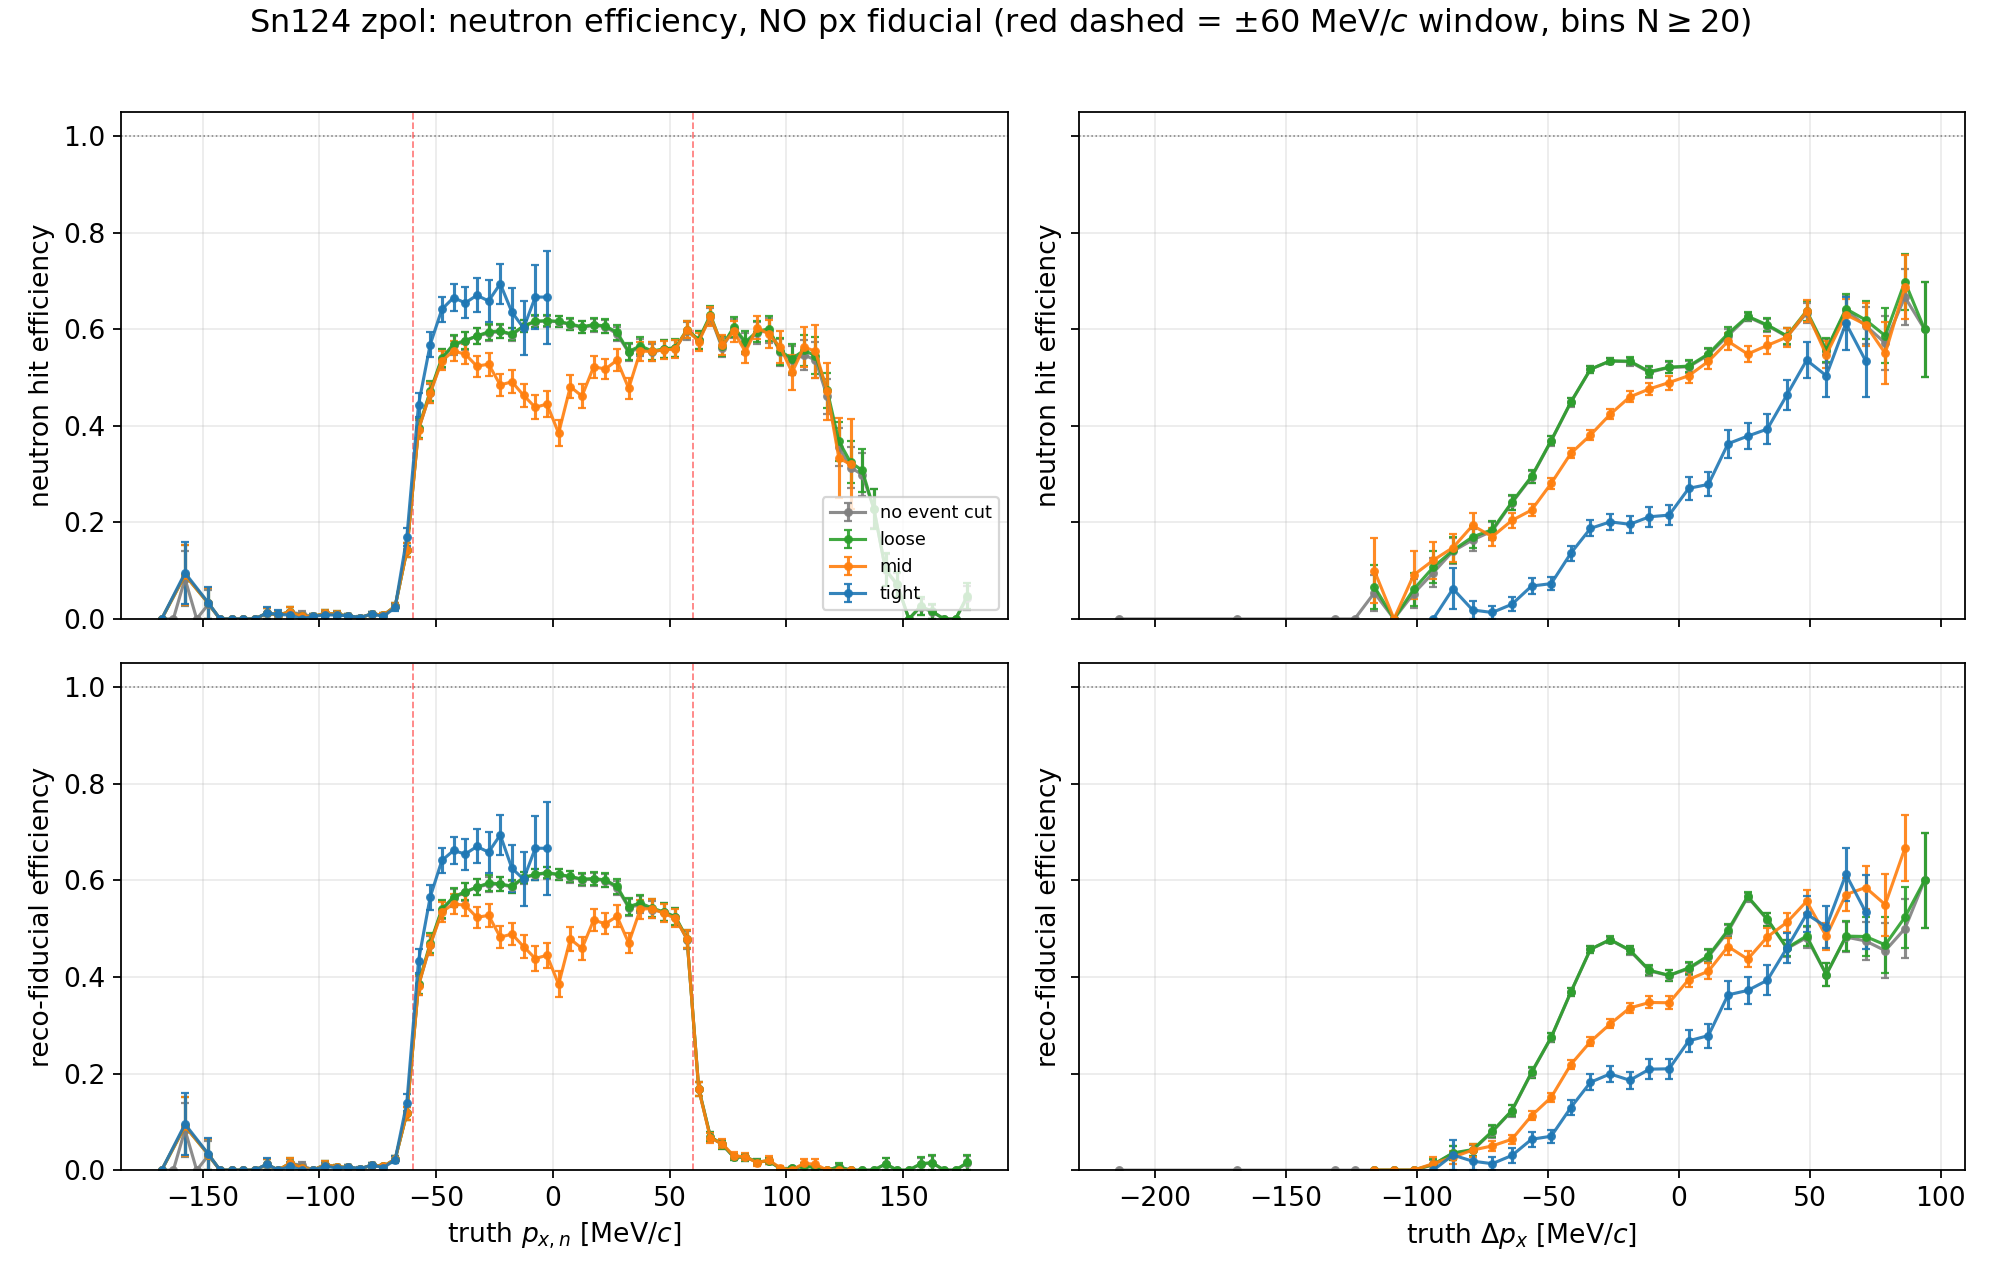
\includegraphics[width=\linewidth]{cut_diagnostics/neutron_efficiency_1d_nofiducial_zpol.png}
  \caption{zpol 的对应全范围效率曲线。}
\end{figure}

\begin{figure}[H]
  \centering
  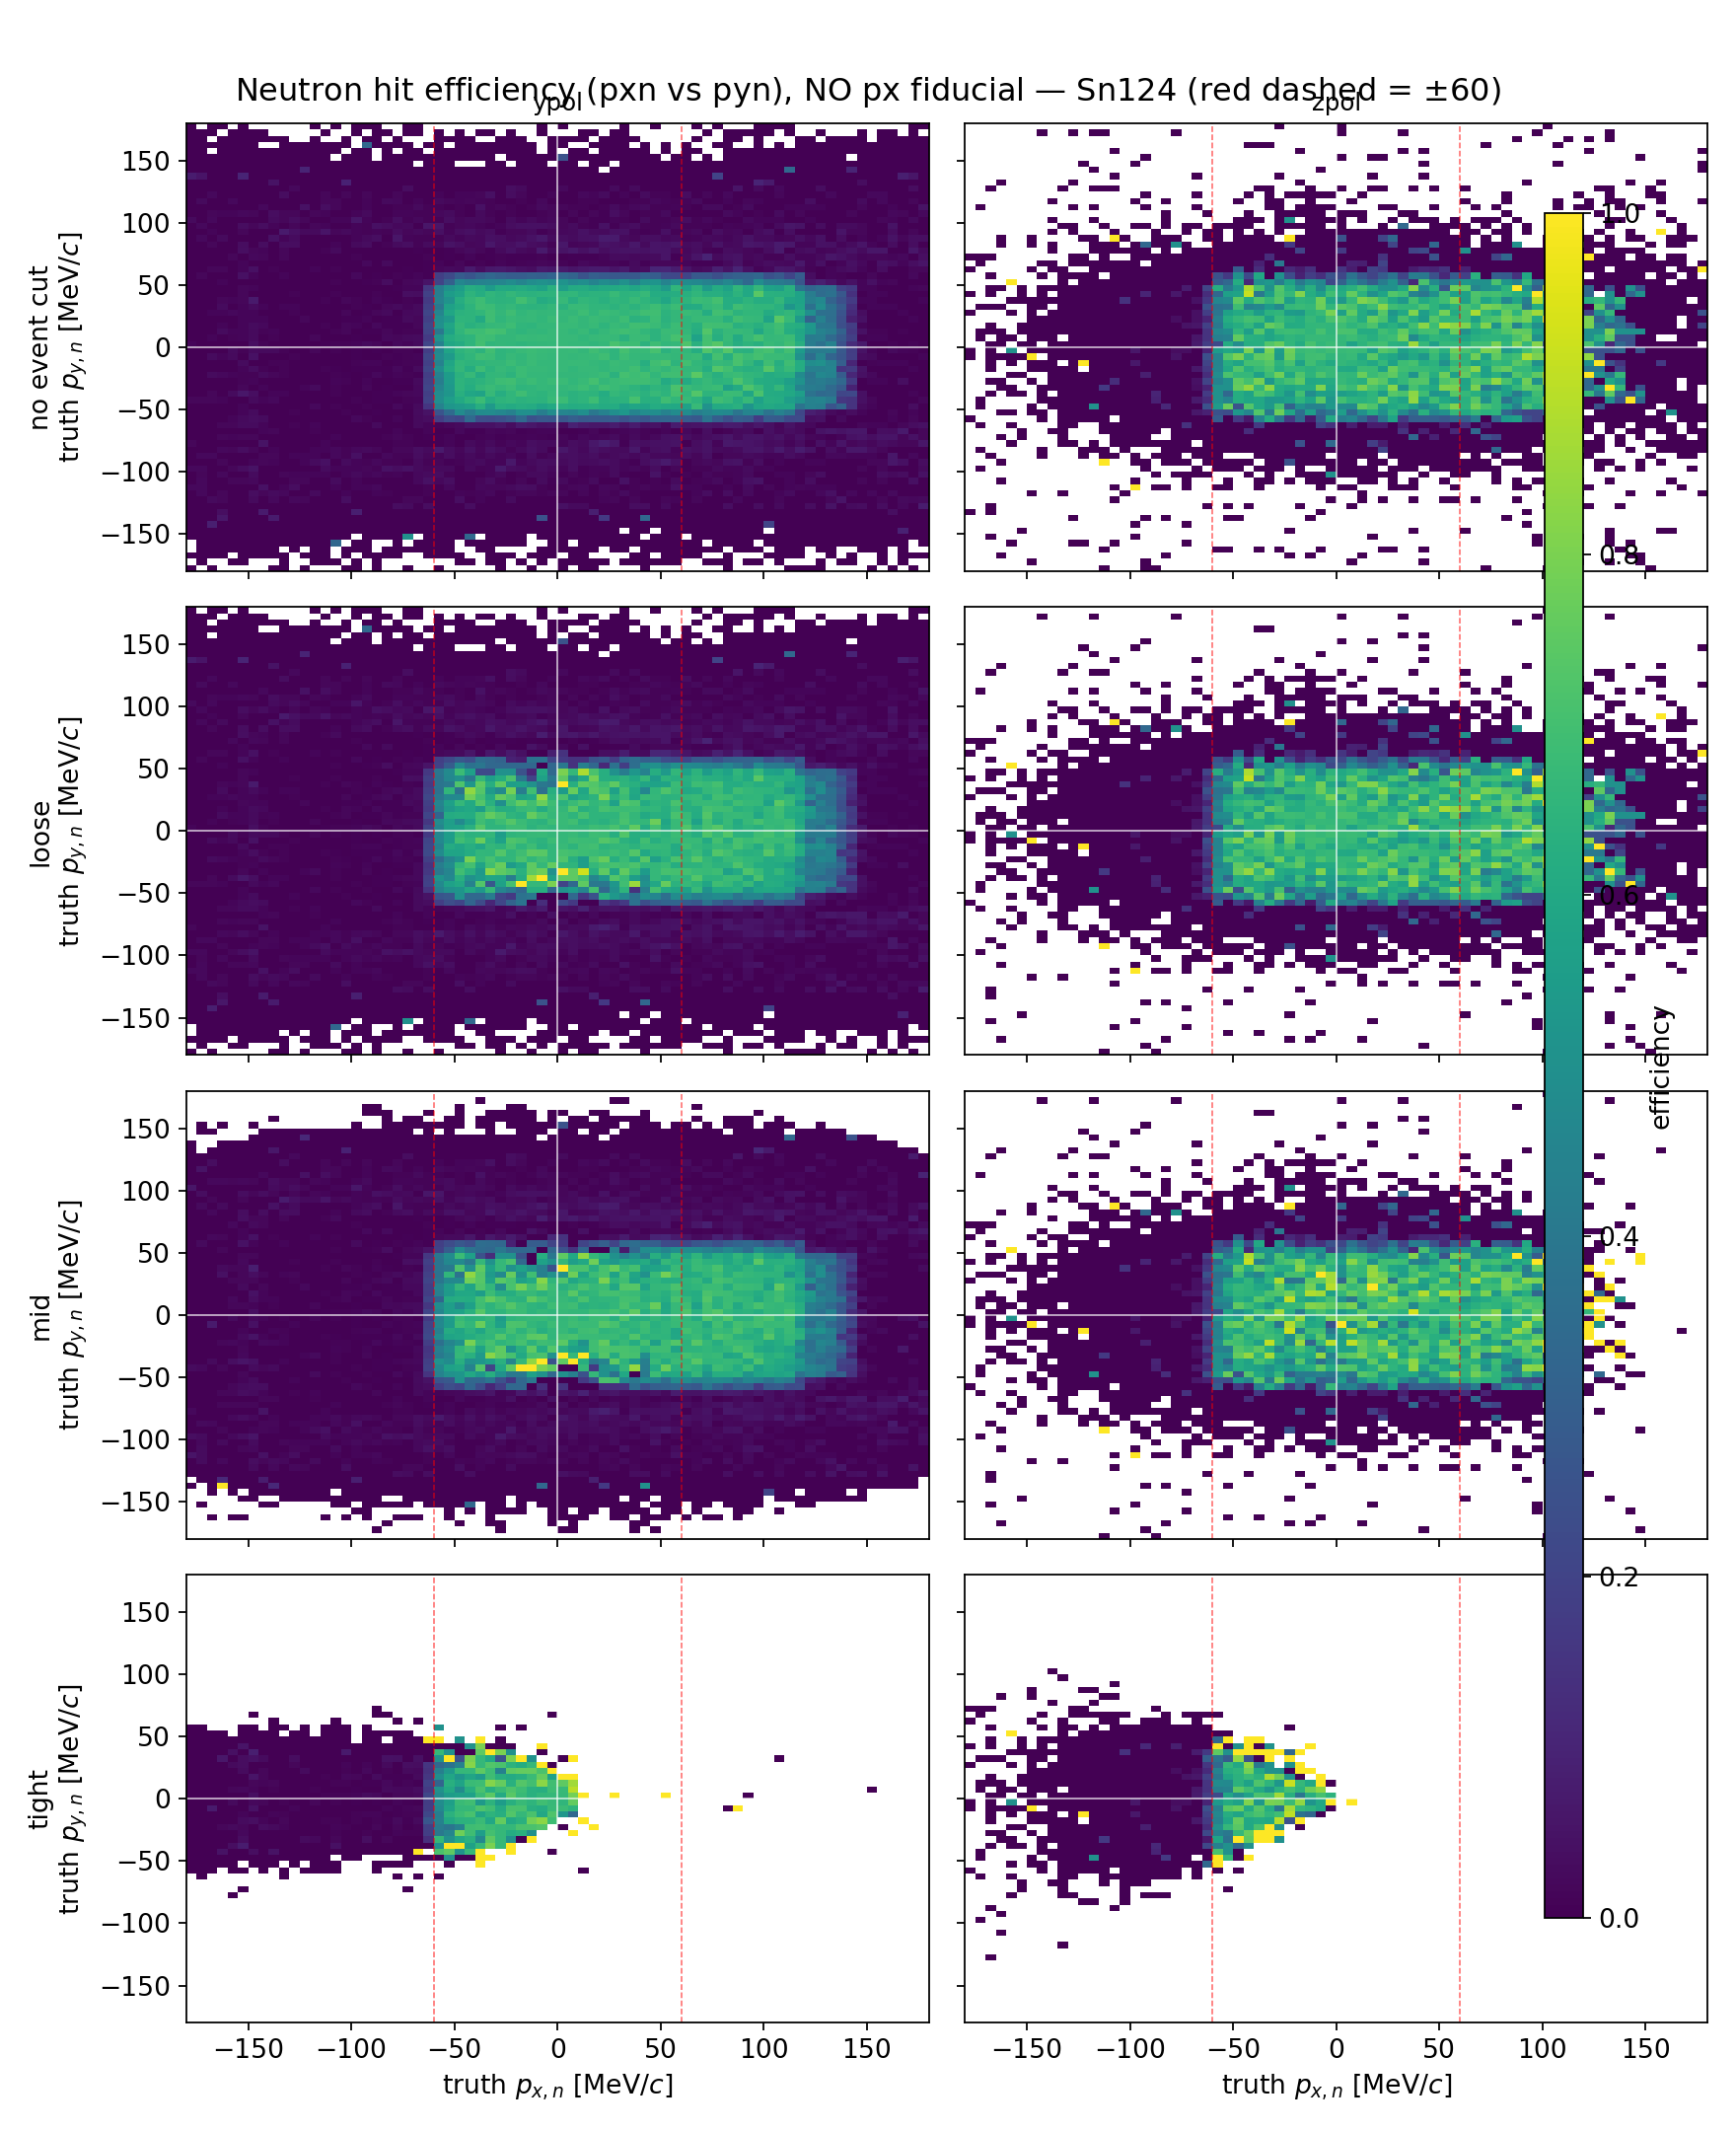
\includegraphics[width=0.82\linewidth]{cut_diagnostics/neutron_efficiency_2d_pxn_vs_pyn_nofiducial.png}
  \caption{无 px fiducial 的 2D neutron hit efficiency ($p_{x,n}$ vs $p_{y,n}$)，按 event-quality cut 分行。红色虚线 = $\pm$60 MeV/$c$。}
\end{figure}

\begin{figure}[H]
  \centering
  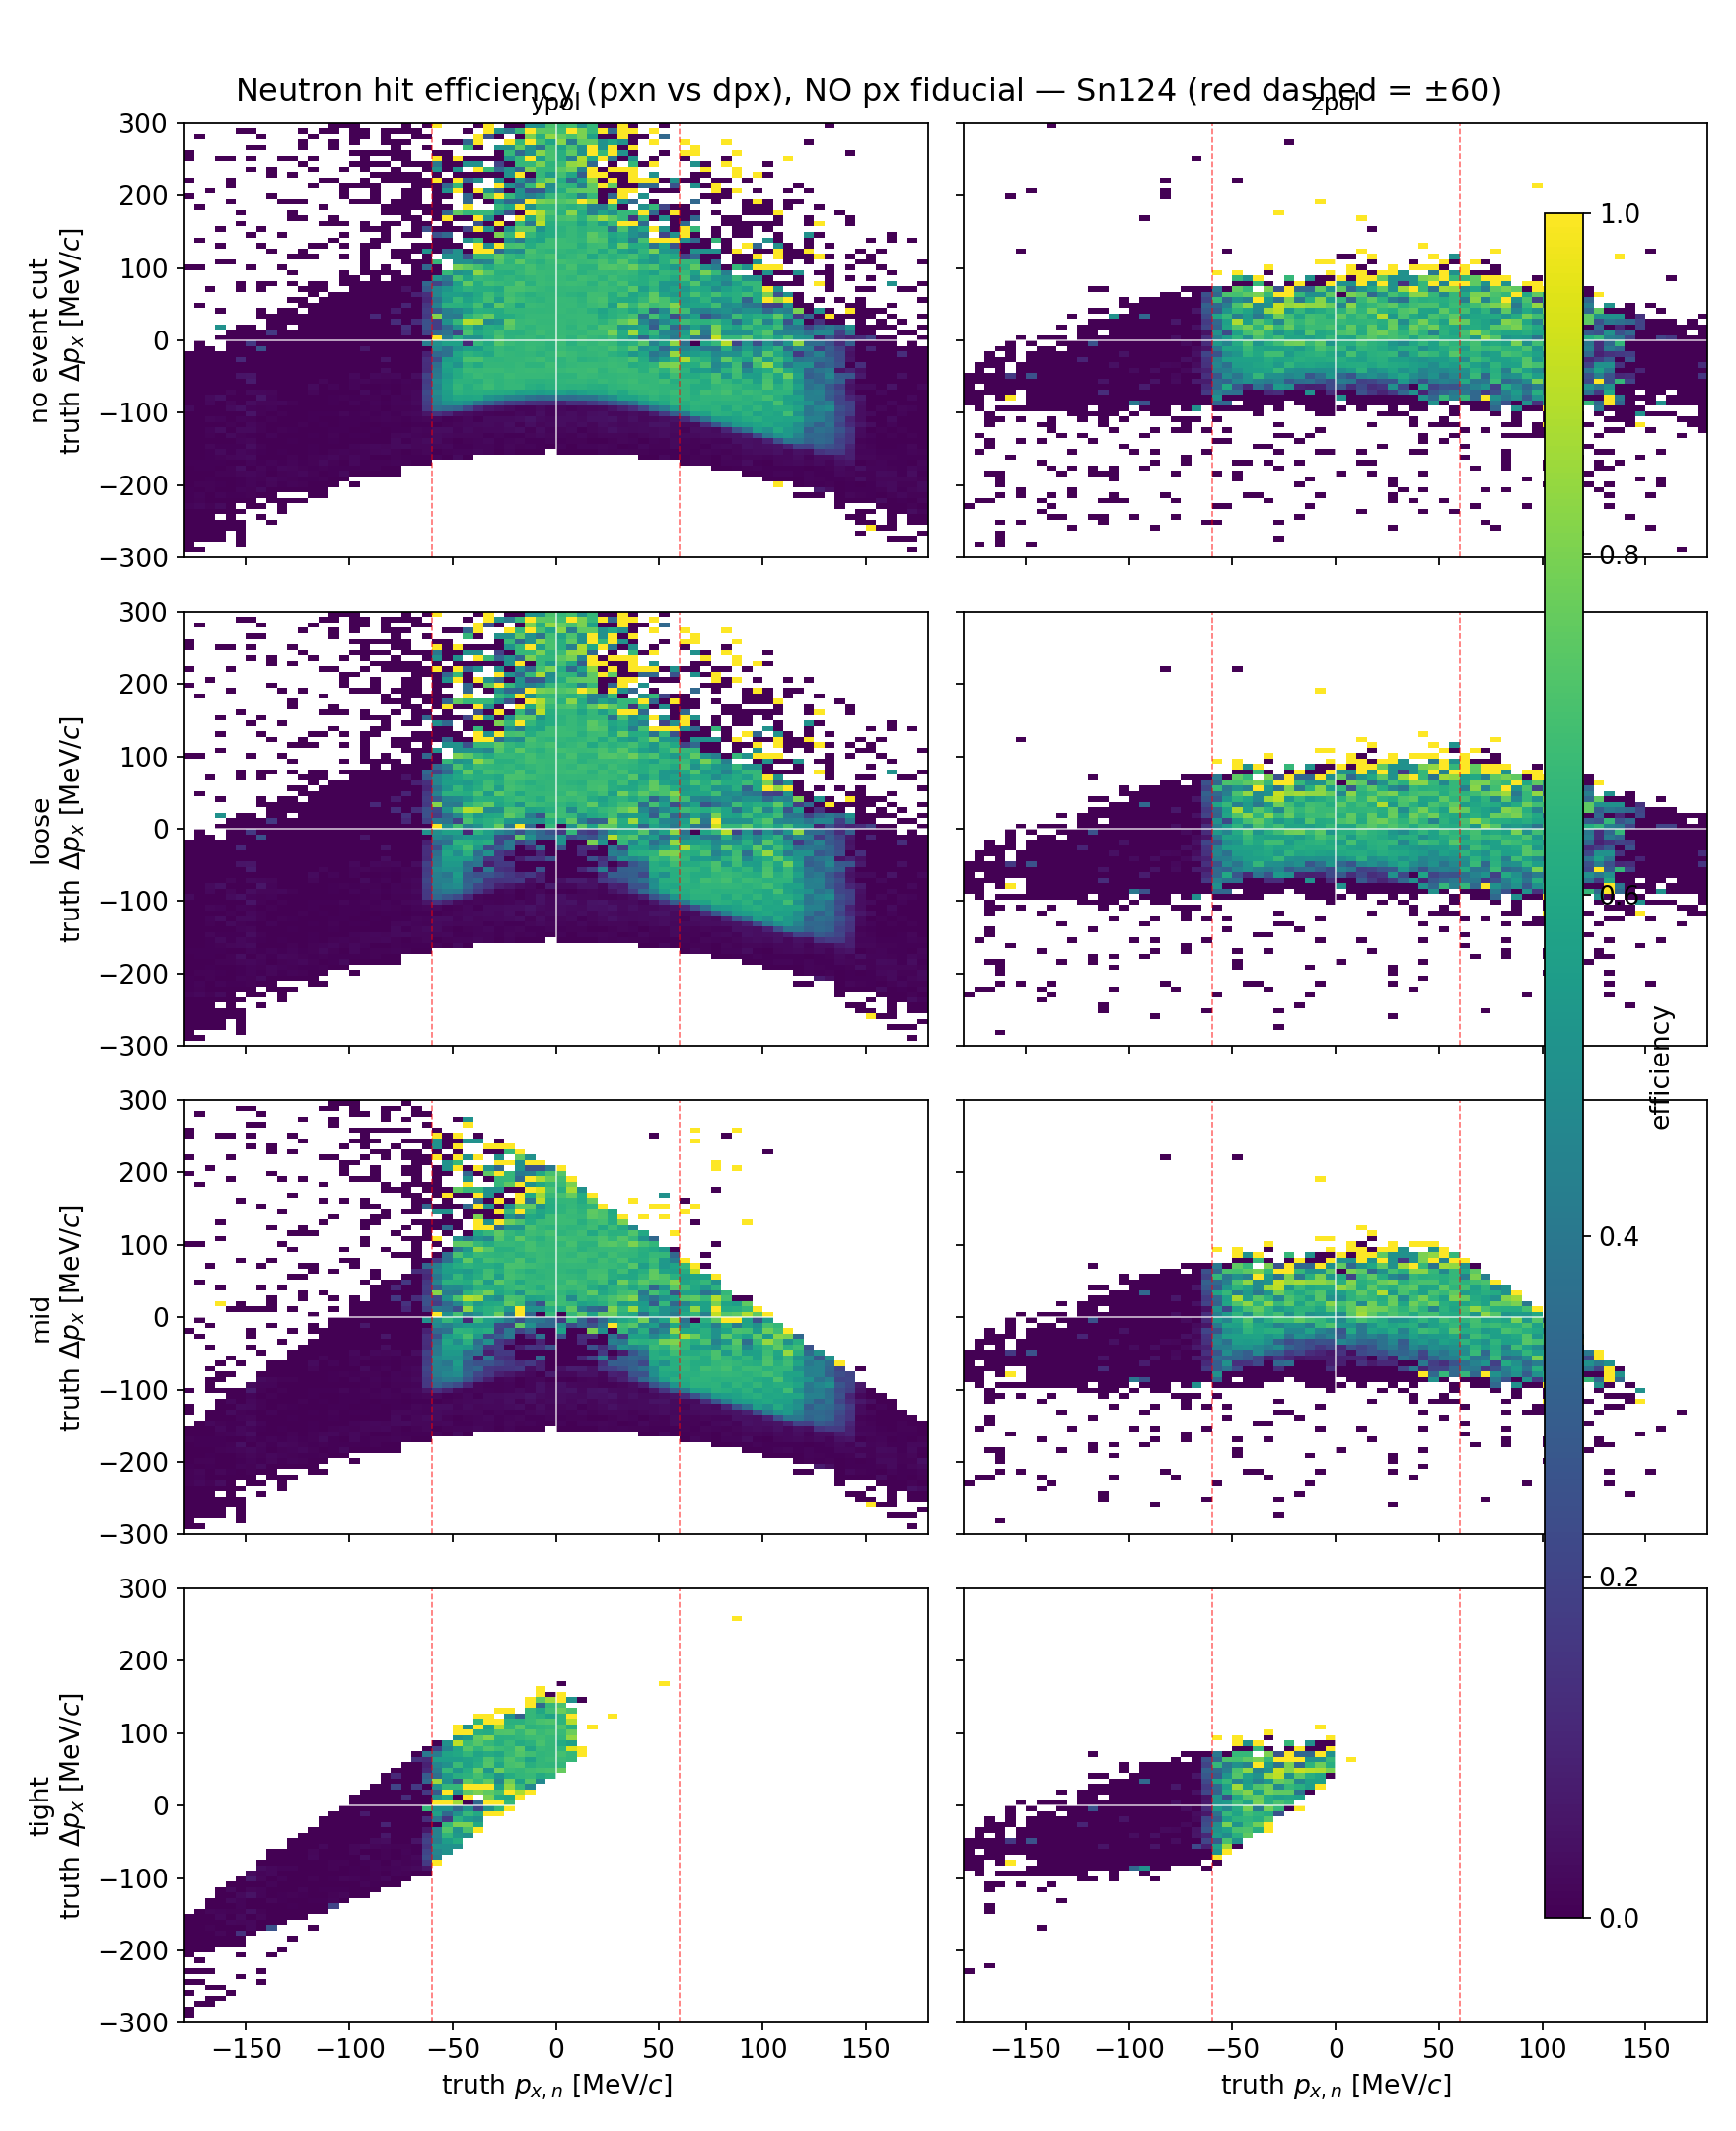
\includegraphics[width=0.82\linewidth]{cut_diagnostics/neutron_efficiency_2d_pxn_vs_dpx_nofiducial.png}
  \caption{同上，$p_{x,n}$ vs $\Delta p_x$。}
\end{figure}

这组图回答的核心问题是: \textbf{为什么需要 px60 cut}。去掉 px fiducial 后可以看到完整的 neutron 效率景观——NEBULA 对正 $p_{x,n}$ 侧的效率较高 ($\sim$0.6--0.7)，但对负 $p_{x,n}$ 且 $|p_{x,n}|>60$ 的区域效率急剧下降 (ypol)。这正是 px100 会保留一个 NEBULA 几乎看不到的负分支、从而扭曲 $R$ 的物理原因。px60 把分析限制在两侧效率都 $>0.5$ 的核心区域，把 sign-dependent efficiency imbalance 控制在可建模范围内。

\section{技术约定: 坐标系、$p_x$ 和反应平面角度}

lab frame 是 Geant4/SAMURAI world frame，也是 NEBULA-Plus macro 里的探测器坐标系: $+Z$ 沿名义束流下游，$+Y$ 竖直，$+X$ 是水平色散方向。下面的 event-display 图横轴是 lab $Z$，纵轴是 lab $X$，所以上方就是 lab $+X$。target/input frame 是生成粒子和 target-momentum reconstruction 使用的动量坐标系。除非图或文字明确写 ``lab''，本报告里的 $p_x$ 都指 $p_x^{\mathrm{tgt}}$，也就是 $p_{x,n}$ fiducial cut 和 response plot 里使用的 target-frame 分量。

当前 target angle 是 $\theta_{\mathrm{tgt}}=3^\circ$。Geant4 primary generator 把粒子放在靶中心，并把输入的 target-frame 动量方向绕 lab $Y$ 轴转 $-\theta_{\mathrm{tgt}}$:
\[
  \mathbf p^{\mathrm{lab}} =
  R_y(-\theta_{\mathrm{tgt}})\,\mathbf p^{\mathrm{tgt}} .
\]
因此 target-frame 正 $p_x$ 表示在共同的 target-angle rotation 之前，动量有指向 lab $+X$ 的分量。对 $p_y=0$ 的简单符号检查，
\[
  p_x^{\mathrm{lab}}
  =
  p_x^{\mathrm{tgt}}\cos\theta_{\mathrm{tgt}}
  -
  p_z^{\mathrm{tgt}}\sin\theta_{\mathrm{tgt}} ,
\]
这里使用的就是模拟里的旋转约定。

\begin{figure}[H]
  \centering
  \begin{minipage}{0.49\linewidth}
    \centering
    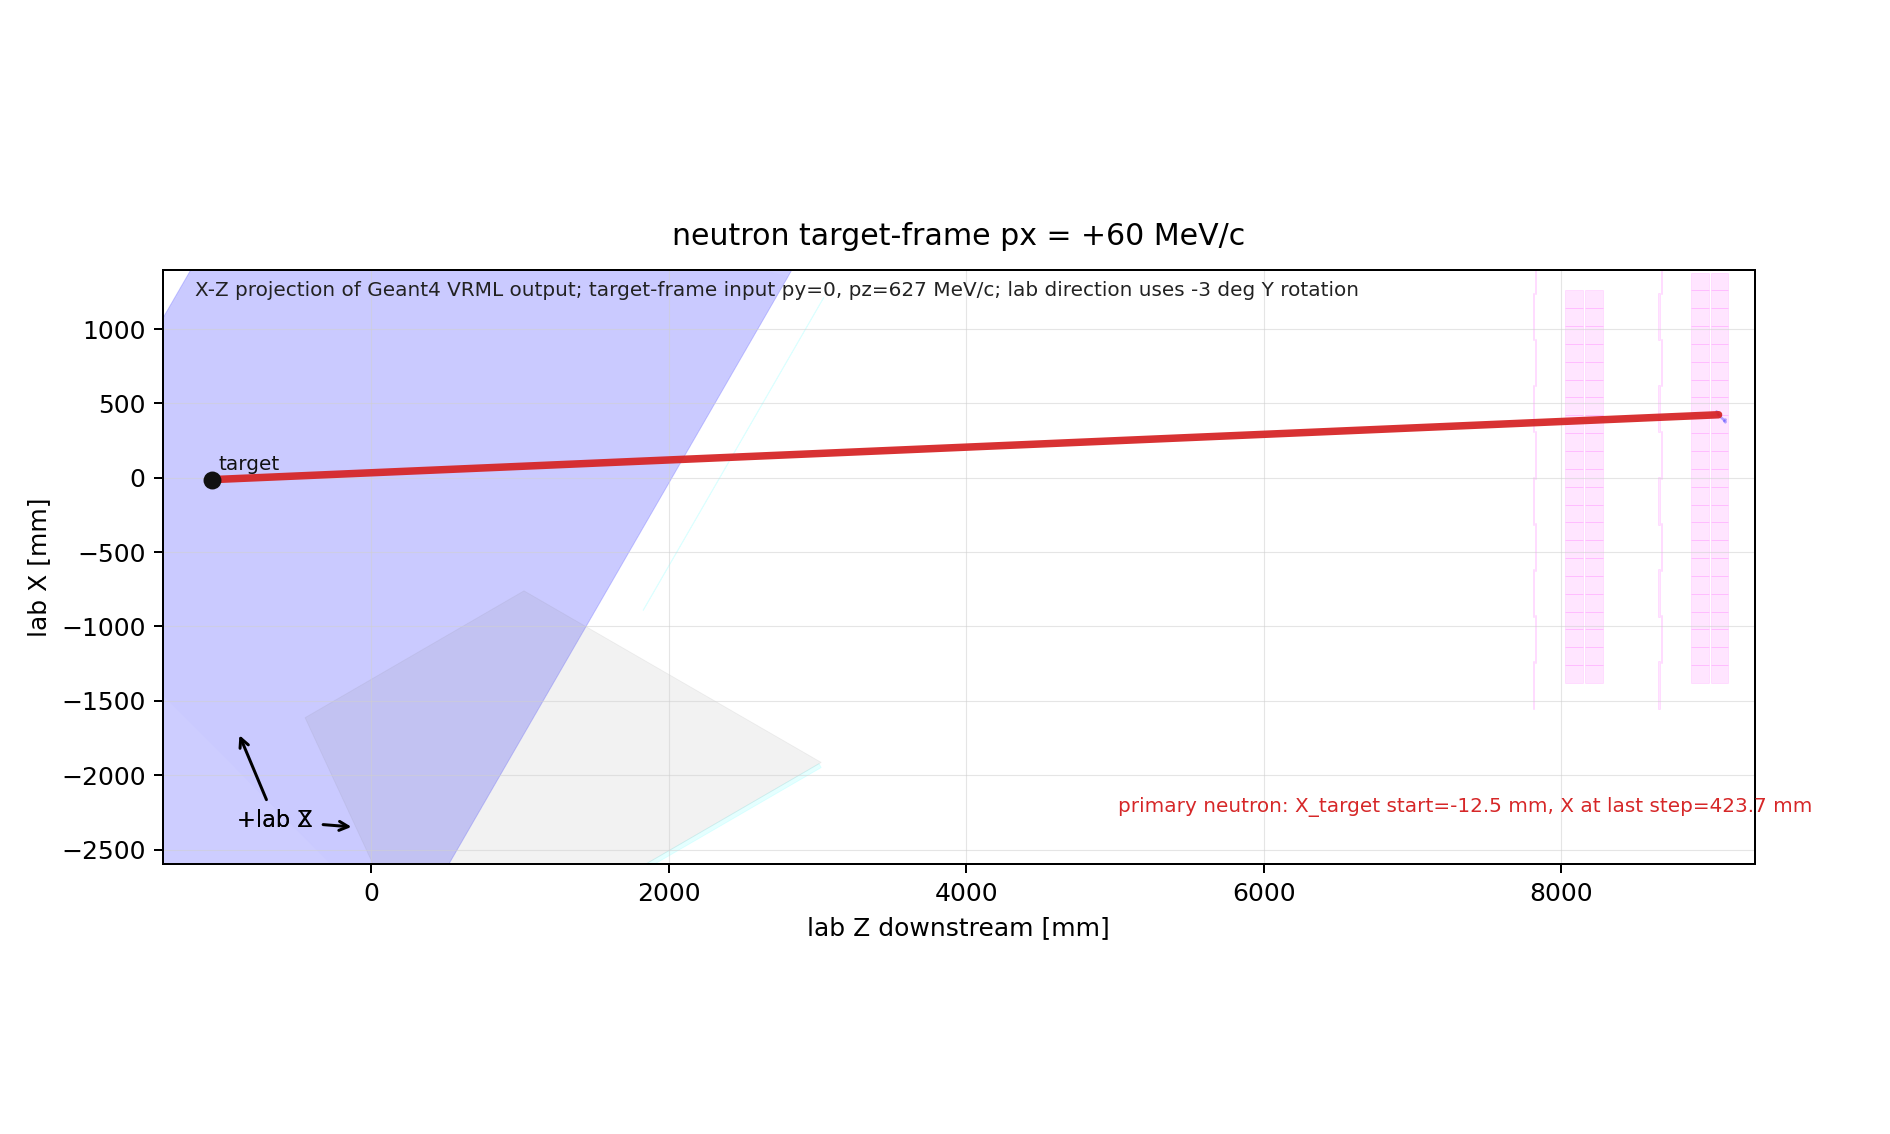
\includegraphics[width=\linewidth]{px_sign_geant4/neutron_px_plus60.png}
  \end{minipage}
  \hfill
  \begin{minipage}{0.49\linewidth}
    \centering
    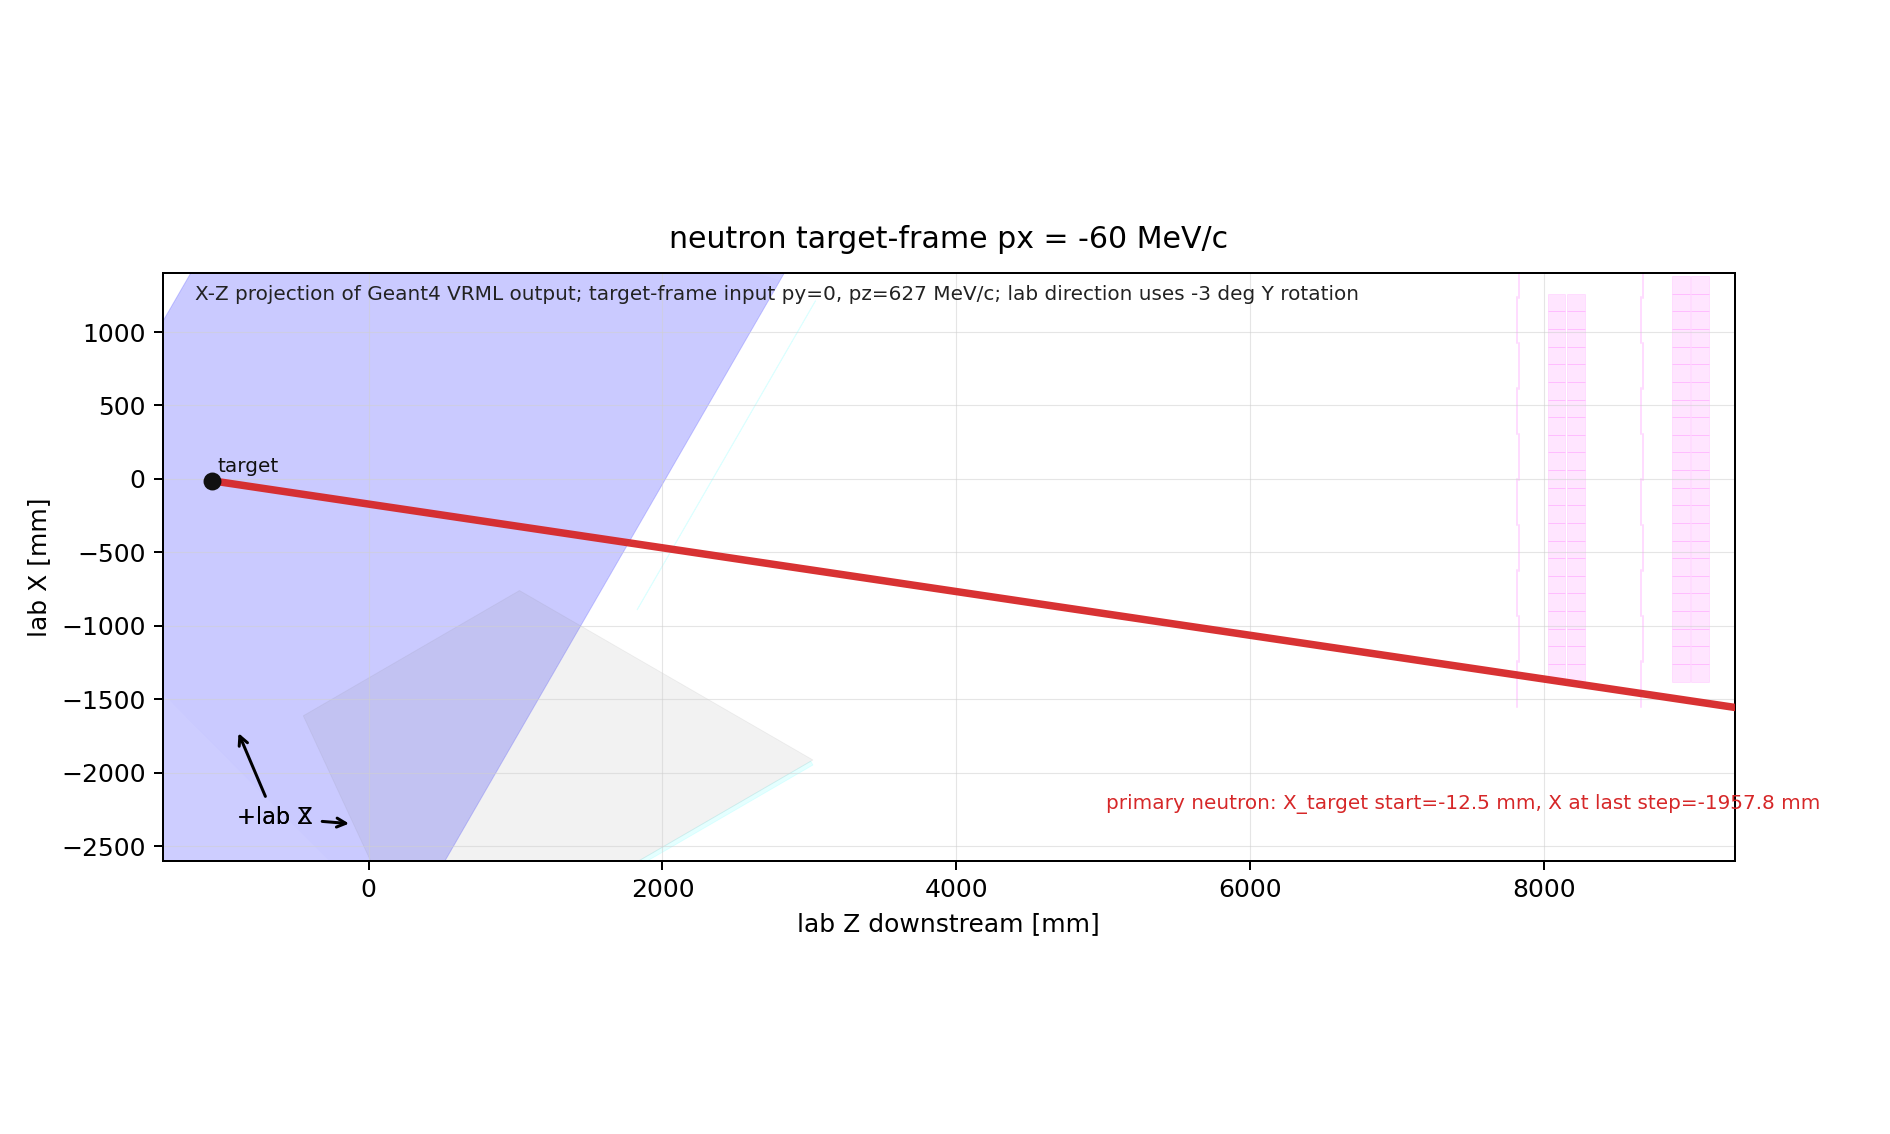
\includegraphics[width=\linewidth]{px_sign_geant4/neutron_px_minus60.png}
  \end{minipage}
  \caption{target-frame neutron $p_x=\pm60$ MeV/$c$ 的 Geant4 WRL-to-PNG 投影，输入为 $p_y=0$、$p_z=627$ MeV/$c$。横轴是 lab $Z$ 下游，纵轴是 lab $X$。正 $p_x^{\mathrm{tgt}}$ 在 $-3^\circ$ target rotation 后仍向 lab $+X$ 一侧偏，负 $p_x^{\mathrm{tgt}}$ 向 lab $-X$ 一侧偏。}
\end{figure}

\begin{figure}[H]
  \centering
  \begin{minipage}{0.49\linewidth}
    \centering
    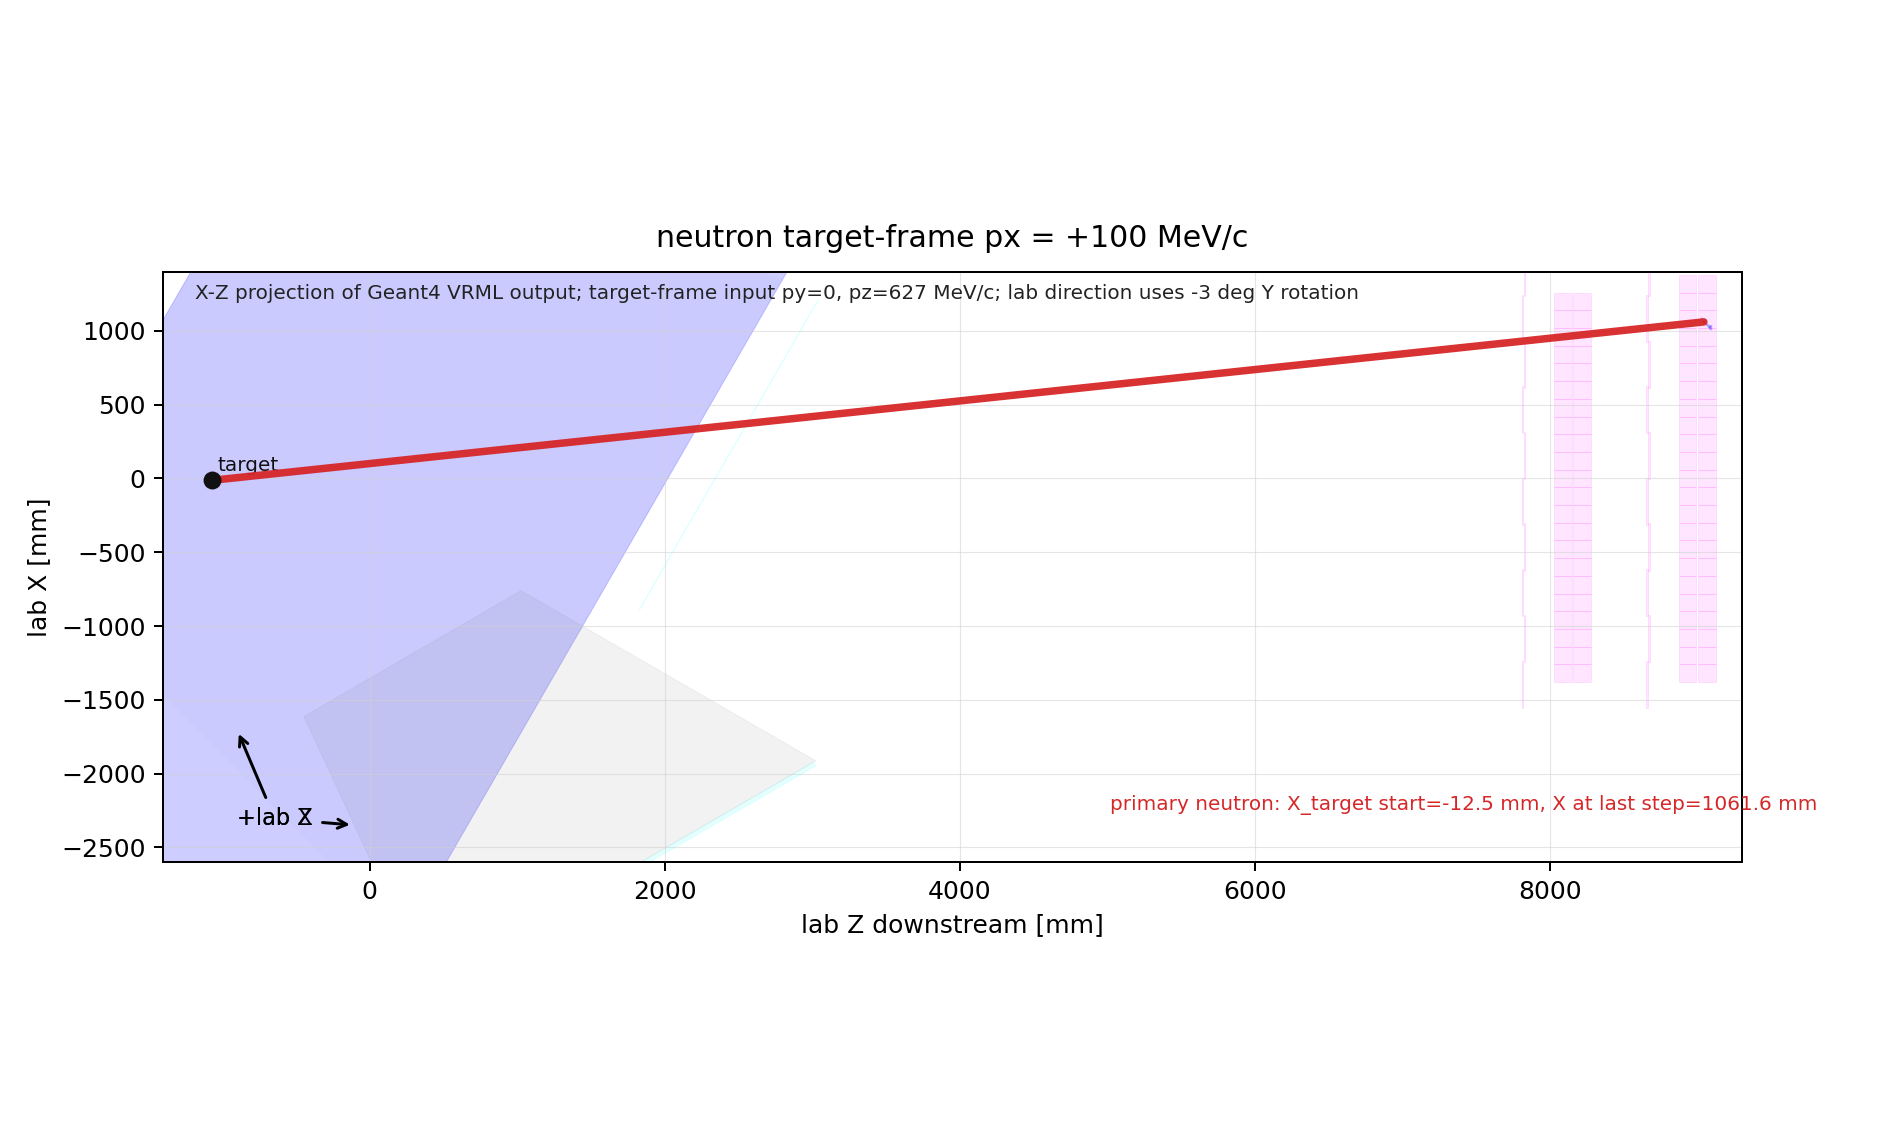
\includegraphics[width=\linewidth]{px_sign_geant4/neutron_px_plus100.png}
  \end{minipage}
  \hfill
  \begin{minipage}{0.49\linewidth}
    \centering
    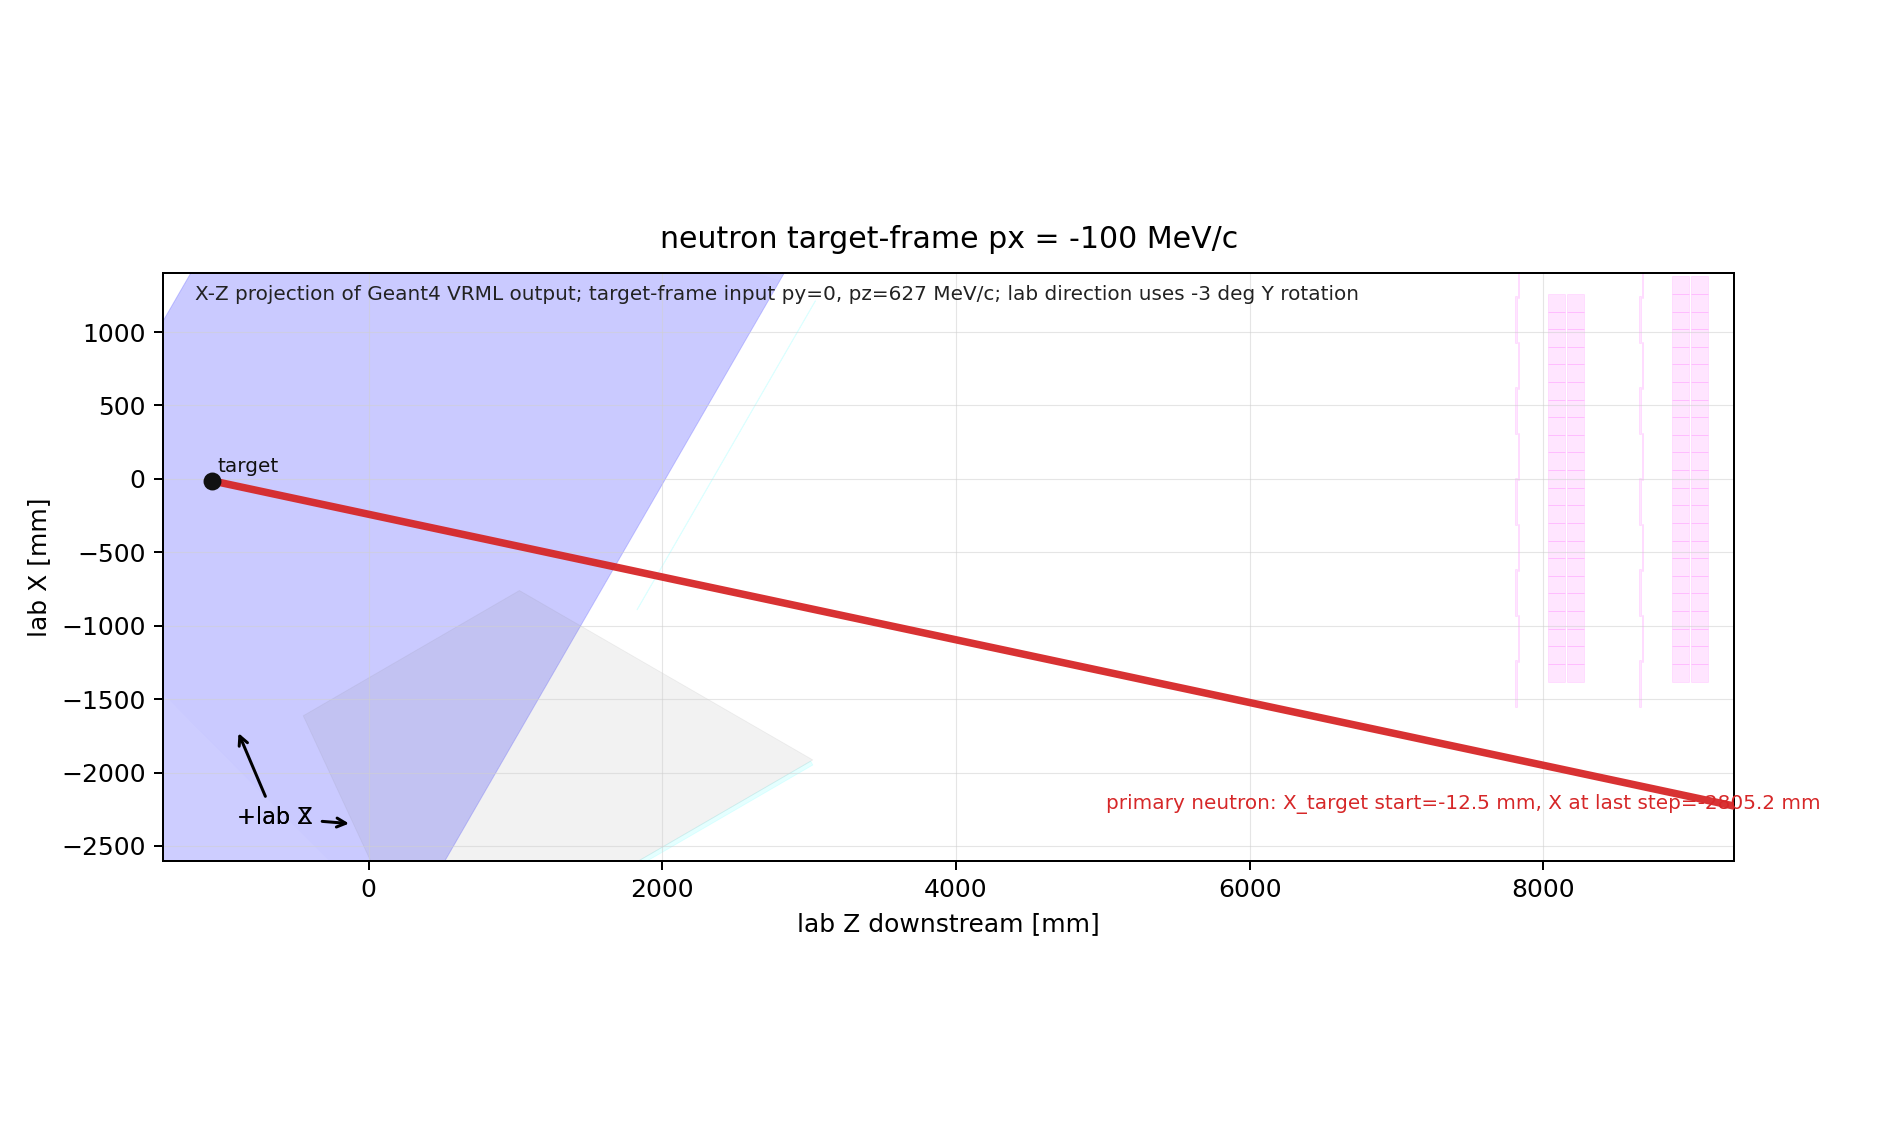
\includegraphics[width=\linewidth]{px_sign_geant4/neutron_px_minus100.png}
  \end{minipage}
  \caption{同样的 Geant4 符号检查，target-frame neutron $p_x=\pm100$ MeV/$c$。更大的 $|p_x|$ 给出更大的 lab-$X$ 偏转，说明重建 $p_{x,n}$ 图中使用的正负号约定是自洽的。}
\end{figure}

这里有两种反应平面角度，不能混用。第一种是 generator/model angle $b_\phi$，它来自 QMD/event metadata；在 y-pol raw sample 中它等于记录的 \texttt{rpphi} modulo $2\pi$，随机旋转样本中则使用 event record 里的 randomized plane angle。这个角是 truth/model plane label，适合做 generator consistency check。

当前 folded observable 使用的是逐事件的运动学平面。定义
\[
  \mathbf k_{\mathrm{out}}
  =
  \mathbf p_p + \mathbf p_n,
  \qquad
  \mathbf k_{\mathrm{out},T}
  =
  (k_{\mathrm{out},x}, k_{\mathrm{out},y}) .
\]
因为 $\mathbf k_{\mathrm{in}}$ 定义 target-frame 的束流轴，$(\mathbf k_{\mathrm{in}},\mathbf k_{\mathrm{out}})$ 反应平面的方位角就是
\[
  \phi_k
  =
  \operatorname{atan2}
  \left(k_{\mathrm{out},y}, k_{\mathrm{out},x}\right)
  =
  \operatorname{atan2}
  \left(p_{y,p}+p_{y,n}, p_{x,p}+p_{x,n}\right).
\]
如果改用 momentum transfer $\mathbf q=\mathbf k_{\mathrm{in}}-\mathbf k_{\mathrm{out}}$ 来定义横向方向，那么横向方位角会相差 $\pi$；这个约定不能和当前 $R$ 定义混在一起。

$\Delta p_x$ 使用的旋转是
\[
  \begin{pmatrix}
    p_x^{\mathrm{rot}} \\
    p_y^{\mathrm{rot}}
  \end{pmatrix}
  =
  R_z(-\phi_k)
  \begin{pmatrix}
    p_x \\
    p_y
  \end{pmatrix}
  =
  \begin{pmatrix}
    p_x\cos\phi_k + p_y\sin\phi_k \\
    -p_x\sin\phi_k + p_y\cos\phi_k
  \end{pmatrix}.
\]
最终观测量定义为
\[
  \Delta p_x
  =
  p_{x,p}^{\mathrm{rot}} - p_{x,n}^{\mathrm{rot}},
  \qquad
  R
  =
  \frac{N(\Delta p_x>0)}{N(\Delta p_x<0)} .
\]

\section{还缺什么}

当前不能过度宣称的部分:
\begin{itemize}
  \item $\eta_{\mathrm{coin}}=4.65\%$ 仍是 manuscript planning anchor。本地 selected-breakup validation 可复现的是约 37.9\% acceptance，两者口径不同，proposal 里必须写清楚。
  \item Sn112/Sn124 的 target-specific breakup cross section 仍需要用统一 ImQMD shell integration 抽取；本文 Sn112 beamtime 数字暂用 atom-density scaling placeholder，不应作为最终 rate 结论。
  \item 还没有真实实验的 neutron efficiency calibration、time offset、threshold、cross-talk、fake neutron 和 accidental background。
  \item detector response 的系统误差还没有通过 toy closure 或 pseudo-data closure 量化。
  \item 当前报告使用的是 simulation truth-defined cuts 和 reco-defined visible window 的混合诊断；最终实验分析要把所有实验端 cuts 写成 reco-only 版本，并用 simulation 做 truth 对照。
\end{itemize}

\section{推荐给 proposal 或报告的表述}

可以写:
\begin{quote}
在 Sn124 上，经过 NEBULA-Plus detector response、PDC NN proton reconstruction 和 neutron reconstruction 后，\texttt{tight + |p\_x,n|<60 MeV/c} 的 folded $R$ observable 仍保留强 $\gamma$ 依赖。按当前 15 mm/1.2 g Sn target、$1.0\times 10^7$ pps、16 h planning，Sn124 统计量比相邻 $\gamma$ 点 3$\sigma$ 区分所需事件数: ypol 高约两个数量级 ($\sim$99$\times$)，zpol 高约四个数量级 ($\sim$1.4$\times10^4\times$)。Sn112 同口径 folded $R$ 也已计算；若暂用 atom-density scaling placeholder，ypol 最难间隔仍有约 $2.1\times$ 的统计裕量，zpol 裕量约 $3.7\times10^3\times$。因此实验对 $\gamma$ 的约束可行性主要取决于 detector folding 的系统控制，而不是原始统计量。
\end{quote}

不应该写:
\begin{quote}
reco $R$ 已经等于 truth $R$。
\end{quote}

更准确的表述是:
\begin{quote}
实验应比较 folded data 与 folded model；truth-level $R$ 只作为物理解释和 closure-test 参考。
\end{quote}

\end{document}
